\documentclass[letter]{article}

\usepackage[english]{babel}
\usepackage[utf8]{inputenc}
\usepackage{amsmath}
\usepackage[colorinlistoftodos]{todonotes}
\usepackage{makecell}
\usepackage{multirow}
\usepackage{caption}
\usepackage{subcaption}
\usepackage{graphicx}
\usepackage{hyperref}
\usepackage[all]{hypcap}
\usepackage{enumitem}

\newlist{questions}{enumerate}{1}
\setlist[questions, 1]{label = \arabic*}
\newlist{bonus}{enumerate}{1}
\setlist[bonus, 1]{label = Bonus \arabic*}



% Adjust margins
\addtolength{\oddsidemargin}{-0.375in}
\addtolength{\evensidemargin}{-0.375in}
\addtolength{\textwidth}{1in}
\addtolength{\topmargin}{-.5in}
\addtolength{\textheight}{1.5in}

\title{CS 520: Assignment 1 - Path Planning and Search Algorithms}
\author{Haoyang Zhang, Han Wu, Shengjie Li, Zhichao Xu}
\date{\today}

\begin{document}
\maketitle

\section{Introduction, group members and division of workload}
\label{sec:Introduction}

In this group project, apart from implementing DFS, BFS, $ A^* $ with Euclidean Distance Heuristic and $ A^* $ with Manhattan Distance Heuristic, we also did some modification to these algorithms for different performance out of our personal interests.  \\
\begin{tabular}{| p{2.5cm} | p{11.5cm} |}
	\hline
	\makecell[c]{Name \\ RUID} & Workload \\
	\hline
	\makecell[c]{Haoyang Zhang \\ 188008687} & {Implemented DFS, Iterative Deepening DFS, BFS, Bidirectional BFS, Bidirectional $ A^* $, Simulated-Annealing-Based Beam Search and the visualization of maze. Modified DFS to make it able to return optimal path. Added Last-in First-out feature to $ A^* $. Managed to combine Simulated-Annealing-Based Beam Search with Genetic Algorithm. Ran tests for DFS and BFS in question 10. Finished half of the writing of report for part 2.} \\
	\hline
	\makecell[c]{Han Wu \\ 189008460} & {Wrote python scripts for testing the performance of algorithms. Combine the data and generated figures for question 1, 2, 4 and 5. Finished the writing of report for question 1, 2, 4 and 5.} \\
	\hline
	\makecell[c]{Shengjie Li \\ 188008047} & {Implemented $ A^* $ with Euclidean Distance Heuristic, $ A^* $ with Manhattan Distance Heuristic and Genetic Algorithm. Ran tests for $ A^* $ with Euclidean Distance Heuristic and Manhattan Distance inquestion 10. Finished the format design of whole report using \LaTeX. } \\
	\hline
	\makecell[c]{Zhichao Xu \\ 188008912} & {Wrote python scripts for testing the performance of algorithms. Combine the data and generated figures for question 3, 6 and 7. Finished the writing of report for question 3, 6 and 7. Suggested an improvement of $ A^* $ using Chebyshev Distance.} \\
	\hline
\end{tabular}


\section{Part 1: Path Planning}
\label{sec:Part 1: Path Planning}

\begin{questions}
	\item {For each of the implemented algorithms, how large the maps can be ( in terms of dim ) for the algorithm to return an answer in a reasonable amount of time (less than a minute) for a range of possible $ p $ values? Select a size so that running the algorithms multiple times will not be a huge time commitment, but that the maps are large enough to be interesting.} \\
	
	In order to find a reasonable size of the maze, we tested the running time of the algorithm. For each size, we generated 10 mazes and run different algorithms on these 10 mazes. We recorded the average time each algorithm needs to return an answer. The 10 mazes in each test ccould be either solvable or unsolvable. We set $ p $ equals to 0.3 and executed the experiment. \\
	The results are shown below as Table \ref{Table 1}:  \\
	
	\begin{center}
		\label{Table 1}
		\begin{tabular}[h]{| c | c | c | c | c | c | c | c |}
			\hline
			\multicolumn{2}{|c|}{} & \multicolumn{6}{c|}{Size} \\
			\cline{3-8}
			\multicolumn{2}{|c|}{} & 100 & 200 & 400 & 800 & 1600 & 3200 \\
			\hline
			\multirow{5}{*}{Time(s)} & DFS & 0.01942 & 0.07087 & 0.28435 & 0.93919 & 4.5064 & 10.83366 \\
			\cline{2-8}
			 & BFS\textsuperscript{2} & 0.07342 & 0.33946 & 1.73646 & 6.40967 & 25.69253 & 91.73234 \\
			 \cline{2-8}
			 & $ A^* $ Euclidean & 0.07811 & 0.41706 & 1.62604 & 5.97804 & 25.27724 & 100.37974 \\
			 \cline{2-8}
			 & $ A^* $ Manhattan & 0.06093 & 0.29222 & 0.88752 & 3.63068 & 11.147 & 63.8882 \\
			 \cline{2-8}
			 & BFS\textsuperscript{1} & \multicolumn{6}{l|}{254.36093 (size=30)} \\
			 \hline
		\end{tabular}
		\captionof{table}{}
	\end{center}

	DFS was the default setting. BFS1 was the default setting. However, it took too much time. When the size was 30, it took more than 250 seconds to return an answer. So, we changed the settings a little to make BFS acceptable. Here came BFS2. In BFS2, checkFringe=True. The others were also False. A* Euclidean means that A* algorithm used Euclidean Distance as the heuristic function. A* Euclidean means that A Star algorithm used Manhattan Distance as the heuristic function. \\
	
	In the table, we could see that when size becomes large, the average time of returning an answer (whether solvable or unsolvable) increases. BFS2 and A* Euclidean are often the most time-consuming algorithms. We need to run the algorithm repeatedly for the purpose of validations. In order to make it faster in the following test, we chose 200 as the default size of our maze. \\
	
	\item {Find a random map with $ p \approx 0.2 $ that has a path from corner to corner. Show the paths returned for each algorithm. (Showing maps as ASCII printouts with paths indicated is sufficient; however 20 bonus points are available for coding good visualizations.)} \\
	
	In this question, we drew the path of using different algorithms to solve the maze and we studied the effect of different parameters on the problem solving. \\
	We took 20×20 maze as an example. The maze is shown below: \\
	
	\begin{figure}
		\minipage{0.32\textwidth}
		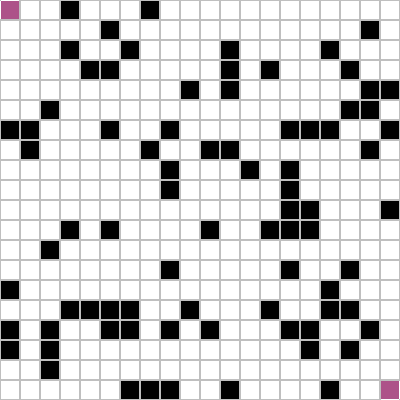
\includegraphics[width=\linewidth]{../pics/question2-1.png}
		\caption{A really Awesome Image}\label{fig:awesome_image1}
		\endminipage\hfill
		\minipage{0.32\textwidth}
		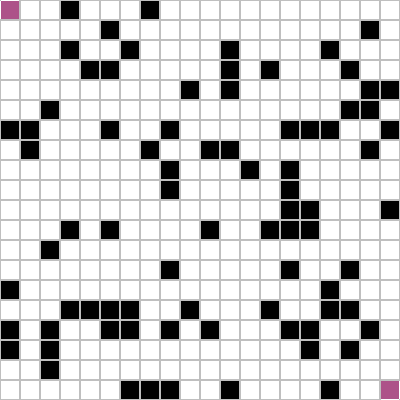
\includegraphics[width=\linewidth]{../pics/question2-1.png}
		\caption{A really Awesome Image}\label{fig:awesome_image2}
		\endminipage\hfill
		\minipage{0.32\textwidth}%
		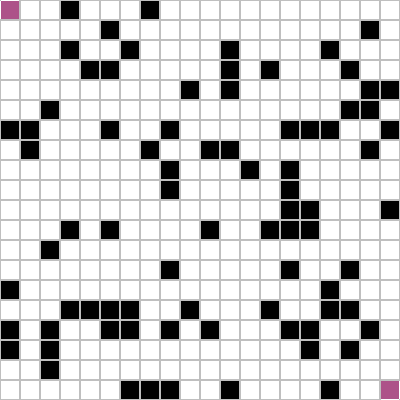
\includegraphics[width=\linewidth]{../pics/question2-1.png}
		\caption{A really Awesome Image}\label{fig:awesome_image3}
		\endminipage
	\end{figure}
	
	TODO \\
	
	
	\item {For a fixed value of dim as determined in Question (1), for each $ p = 0.1, 0.2, 0.3, ... , 0.9 $, generate a number of maps and try to find a path from start to goal - estimate the probability that a random map has a complete path from start to goal, for each value of $ p $. Plot your data. Note that for $ p $ close to 0, the map is nearly empty and the path is clear; for $ p $ close to 1, the map is mostly filled and there is no clear path. There is some threshhold value $ p_0 $ so that for $ p < p_0 $ , there is usually a clear path, and $ p > p_0 $ there is no path. Estimate $ p_0 $ . Which path finding algorithm is most useful here, and why?} \\
	
	In this question, we tried to use a grid-search method first to narrow down the scope of parameters. We used 200 as the mazeSize, and we generated 800 different mazes for the validation of the parameter value. \\
	
	After getting the result, we plotted the rate of successfully finding a path vs the $ p $-value. See Figure \ref{fig:3-1}. \\
	
	\begin{figure}
		\centering
		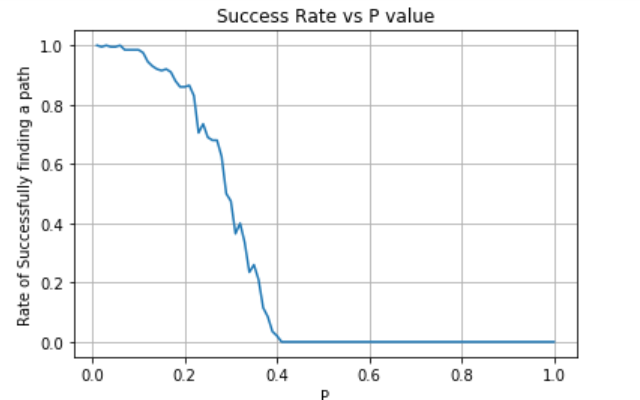
\includegraphics[width=\textwidth]{../pics/question3-1.png}
		\caption{\label{fig:3-1}rate of successfully finding a path vs the $ p $-value.}
	\end{figure}
	
	Then we tried to decrease the step size, and selected the $ p $-value from 0.16 to 0.40 as the $ x $-label to generate a new plot for better analyzing the threshold value here. See Figure \ref{fig:3-2}.\\
	
	\begin{figure}
		\centering
		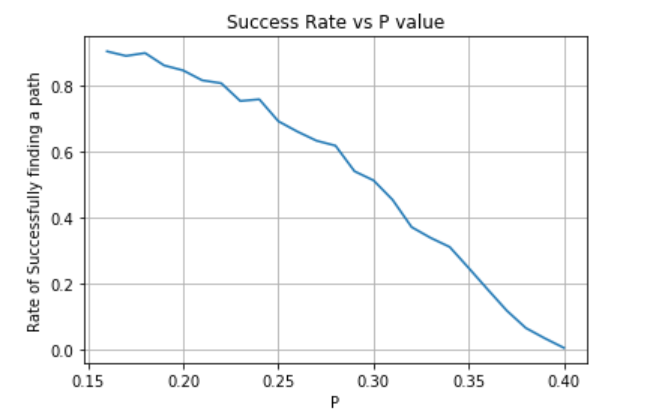
\includegraphics[width=\textwidth]{../pics/question3-2.png}
		\caption{\label{fig:3-2}rate of successfully finding a path vs the $ p $-value.}
	\end{figure}

	After analyzing the result, we notice that the when $ p $ is at 0.40, the success rate stays at 0. Thus we came to conclusion that the threshold is 0.40 for $ p $ here. And to gain a  50\%  of success rate, the $ p $-value should be set to 0.30. \\
	
	In this problem, we used the Bidirectional $ A^* $ method, and the optimal distance function is Manhattan Distance. After the calculation, we found that BD$ A^* $ consumes less time than other algorithms. In this specific problem, because we simplified the settings, we could only move to 4 directions. Manhattan Distance better simulates such scenarios thus it has the best performance here. \\
	
	
	\item {For a range of $ p $ values (up to $ p_0 $), generate a number of maps and estimate the average or expected length of the shortest path from start to goal. You may discard all maps where no path exists. Plot your data. What path finding algorithm is most useful here?} \\
	
	We set $ p $ from 0.05 to 0.35 and the step size was 0.01. For every $ p $, we generated 100 mazes and let the algorithm solve the maze. At this time, all mazes were solvable. We used $ A^* $ with Manhattan Distance Heuristic to solve the problem because $ A^* $ algorithm could return the shortest path. For every $ p $, we took the average of 100 shortest path, and we plotted its relation with the probability $ p $. See Figure \ref{fig:4}: \\
		
	\begin{figure}
		\centering
		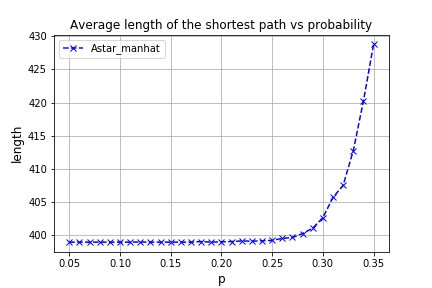
\includegraphics[width=\textwidth]{../pics/question4.png}
		\caption{\label{fig:4}rate of successfully finding a path vs the $ p $-value.}
	\end{figure}

	From Figure \ref{fig:4}, we can see that when $ p $ is less than 0.2, the average shortest is the same. Actually, it equals to the length of the shortest path from the upper left to the lower down. When $ p $ becomes greater, the average length rises fast. When $ p $ is beyond $ p_0 $, the average rises fast. \\
	
	\item {For a range of $ p $ values (up to $ p_0 $ ), estimate the average length of the path generated by $ A^* $ from start to goal (for either heuristic). Similarly, for the same $ p $ values, estimate the average length of the path generated by DFS from start to goal. How do they compare? Plot your data.} \\
	
	We generated 100 mazes under different $ p $ and used 3 algorithms -- $ A^* $ with Euclidean Distance Heuristic, $ A^* $ with Manhattan Distance Heuristic, and DFS(quickGoal = True, randomWalk = True) to solve the mazes. All mazes are solvable. We calculated the average path of each algorithm and plot them together. The result is shown in Figure \ref{fig:5}: \\
	
	\begin{figure}
		\centering
		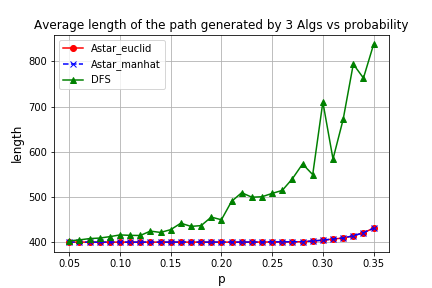
\includegraphics[width=\textwidth]{../pics/question5.png}
		\caption{\label{fig:5}rate of successfully finding a path vs the $ p $-value.}
	\end{figure}
	
	From Figure \ref{fig:5}, we can see that $ A^* $ with Euclidean Distance Heuristic and $ A^* $ with Manhattan Distance Heuristic have the same average shortest path. It is easy to understand this result because $ A^* $ returns the shortest path no matter what heuristic function is used. The average length of DFS is larger than $ A^* $. DFS is fast, but it can’t return the shortest path when it is not optimized. When $ p $ is greater than 0.2, the difference increases quickly. When $ p $ is large, there exists oscillation in the average length of DFS. However, we could come to conclusion that the overall trend is rising. \\
	
	
	\item {For a range of $ p $ values (up to $ p_0 $), estimate the average number of nodes expanded in total for a random map, for $ A^* $ using the Euclidean Distance as the heuristic, and using the Manhattan Distance as the heuristic. Plot your data. Which heuristic typically expands fewer nodes? Why? What about for $ p $ values above $ p_0 $?}
	
	In this question, we generated 200 different mazes to calculate our result and the mazeSize we used is 200×200 here. We used the Euclidean distance as the distance function. The result is demonstrated below as Figure \ref{fig:6-1}. \\
	
	\begin{figure}
		\centering
		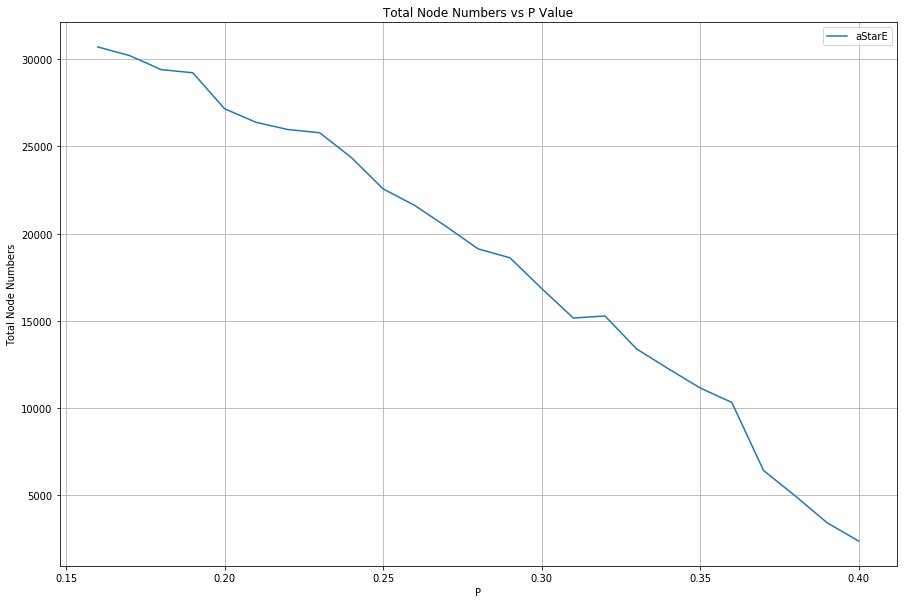
\includegraphics[width=\textwidth]{../pics/question6-1.png}
		\caption{\label{fig:6-1} $ A^* $ with Euclidean Distance Heuristic.}
	\end{figure}
	
	Note that LIFO is our special bool parameter. When LIFO=True, for nodes whose heuristic values are same, the last node entering the priority queue gets popped first. \\
	
	When we used the Manhattan Distance, we conducted two tests. Figure \ref{fig:6-2} was the results of LIFO=True and Figure \ref{fig:6-3} was the results of LIFO=False. \\
	
	\begin{figure}
		\centering
		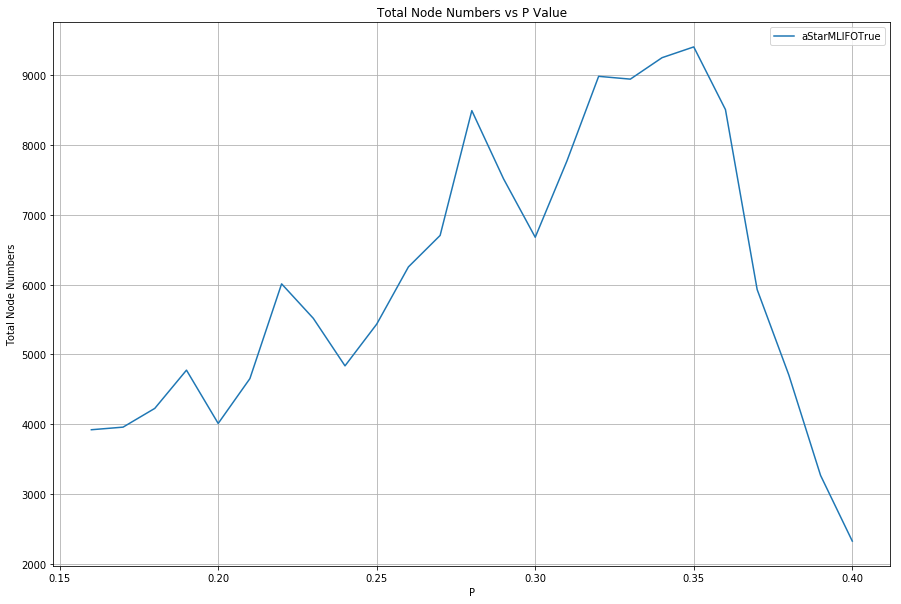
\includegraphics[width=\textwidth]{../pics/question6-2.png}
		\caption{\label{fig:6-2} $ A^* $ with Manhattan Distance Heuristic when LIFO=True.}
	\end{figure}

	\begin{figure}
		\centering
		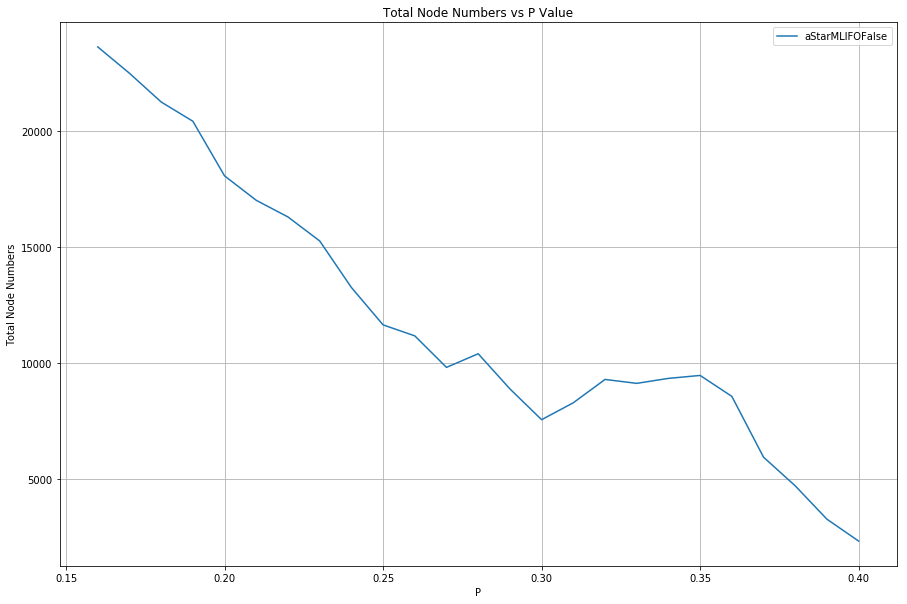
\includegraphics[width=\textwidth]{../pics/question6-3.png}
		\caption{\label{fig:6-3}$ A^* $ with Manhattan Distance Heuristic when LIFO=False.}
	\end{figure}

	In this scenario, Manhattan distance when LIFO=True clearly expands fewer nodes. This is because that Manhattan is a better simulation in this scenario. We simplified the situation such that the node could only explore four directions, which suits the way M distance works. As for LIFO, when $ p $ is small enough, the whole maze almost has no walls. In this case, almost every node has the same cost thus LIFO is similar to DFS, while FIFO could be regarded as BFS. \\
	
	For the Total Node Numbers after $ p_0 $, we have Figure \ref{fig:6-4}, Figure \ref{fig:6-5} and Figure \ref{fig:6-6}: \\
	
	\begin{figure}
		\centering
		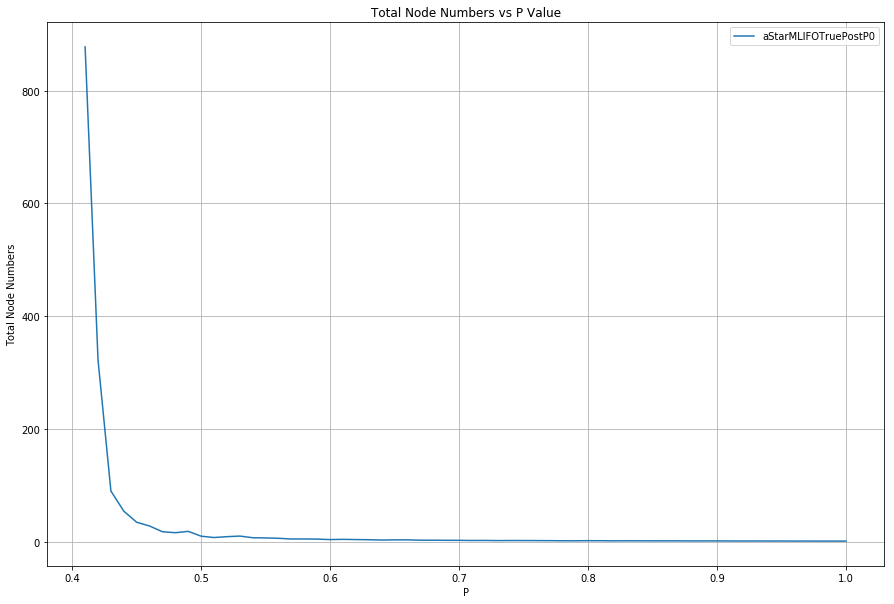
\includegraphics[width=\textwidth]{../pics/question6-4.png}
		\caption{\label{fig:6-4} $ A^* $ with Manhattan Distance Heuristic when LIFO=True and $ p >= p_0 $.}
	\end{figure}
	
	\begin{figure}
		\centering
		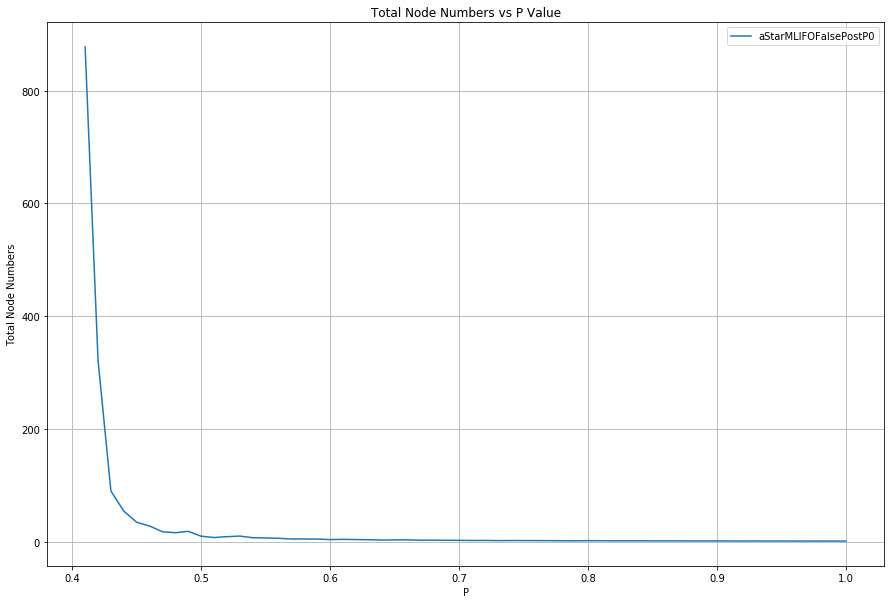
\includegraphics[width=\textwidth]{../pics/question6-5.png}
		\caption{\label{fig:6-5}$ A^* $ with Manhattan Distance Heuristic when LIFO=False and $ p >= p_0 $.}
	\end{figure}

	\begin{figure}
		\centering
		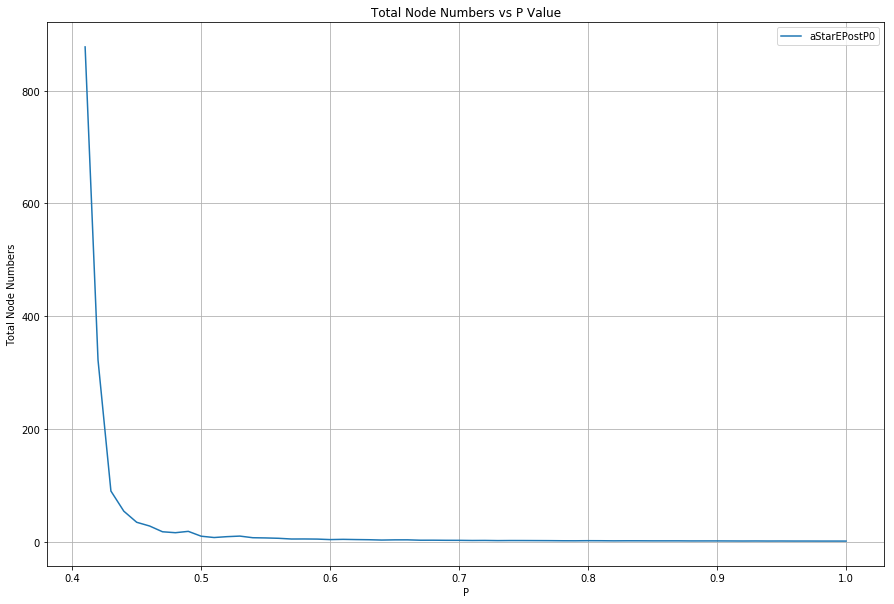
\includegraphics[width=\textwidth]{../pics/question6-6.png}
		\caption{\label{fig:6-6} $ A^* $ with Euclidean Distance Heuristic when $ p >= p_0 $.}
	\end{figure}
	
	From these figures, we could tell when $ p >= p_0 $, their shape are similar. \\
	
	\item {For a range of $ p $ values (up to $ p_0 $), estimate the average number of nodes expanded in total for a random map by DFS and by BFS. Plot your data. Which algorithm typically expands fewer nodes? Why? How does either algorithm compare with $ A^* $ in Question (6)?} \\
	
	In this question, we generated 200 different mazes to calculate our result and the mazeSize we used is 200×200 here.  The result for DFS is shown as Figure \ref{fig:7-1}: \\
	
	\begin{figure}
		\centering
		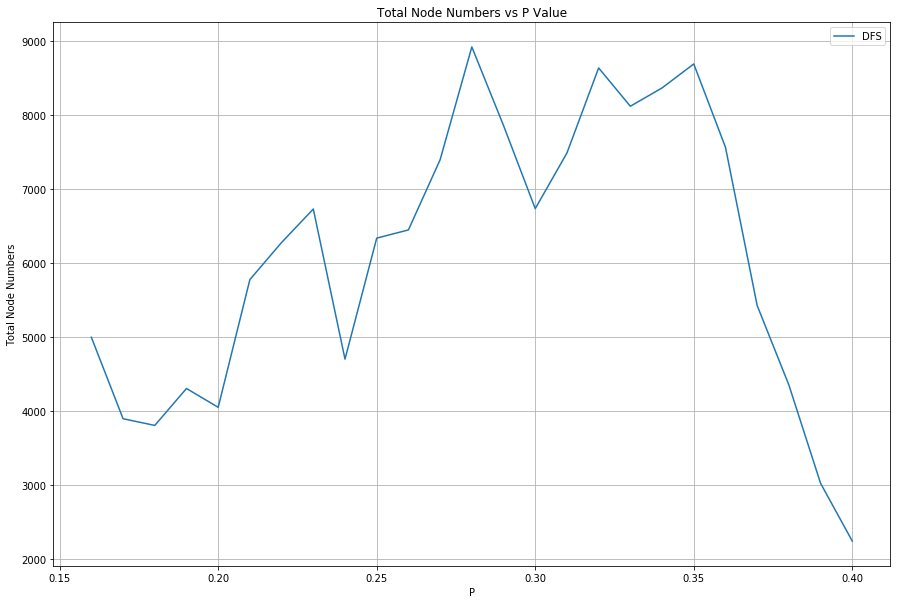
\includegraphics[width=\textwidth]{../pics/question7-1.png}
		\caption{\label{fig:7-1} Average number of nodes expanded for different $ p $ using DFS.}
	\end{figure}

	When we used the BFS, the result is shown as Figure \ref{fig:7-2}: \\
	
	\begin{figure}
		\centering
		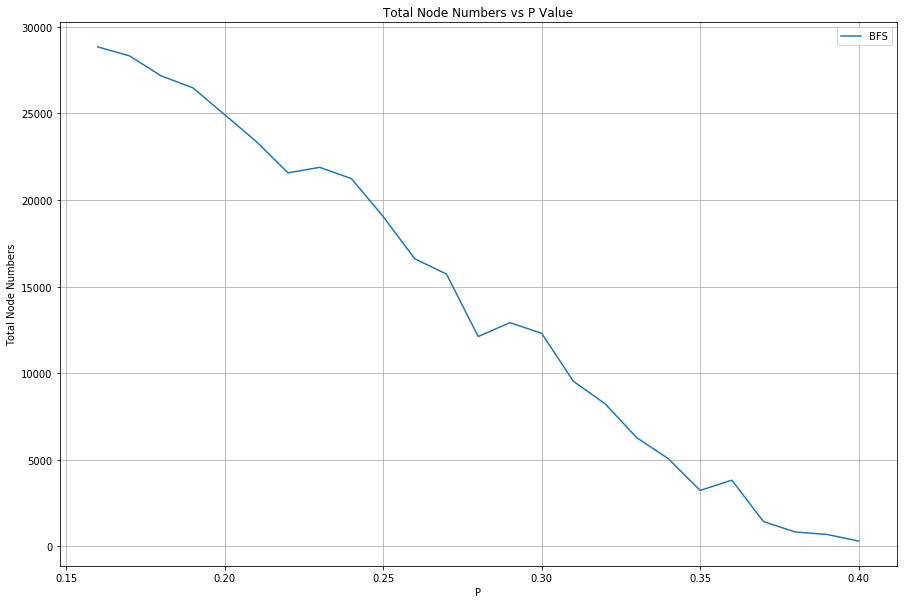
\includegraphics[width=\textwidth]{../pics/question7-2.png}
		\caption{\label{fig:7-2} Average number of nodes expanded for different $ p $ using BFS.}
	\end{figure}

	When $ p $ is low, DFS does not need to trackback for a lot of times. As $ p $ increases, DFS needs to traceback more. Such that the nodes DFS explores increases as $ p $-value grows. Also, DFS performs better than BFS. When DFS explores a path, it will go down the path until it come to a dead end. At the same time, BFS will explore all the nodes it is adjacent to. In the maze-exploration problem, the correct path often exists in the middle of the nodes, thus typically DFS overperforms BFS. \\
	
	To draw the comparison, we have Figure \ref{fig:7-3}: \\
	
	\begin{figure}
		\centering
		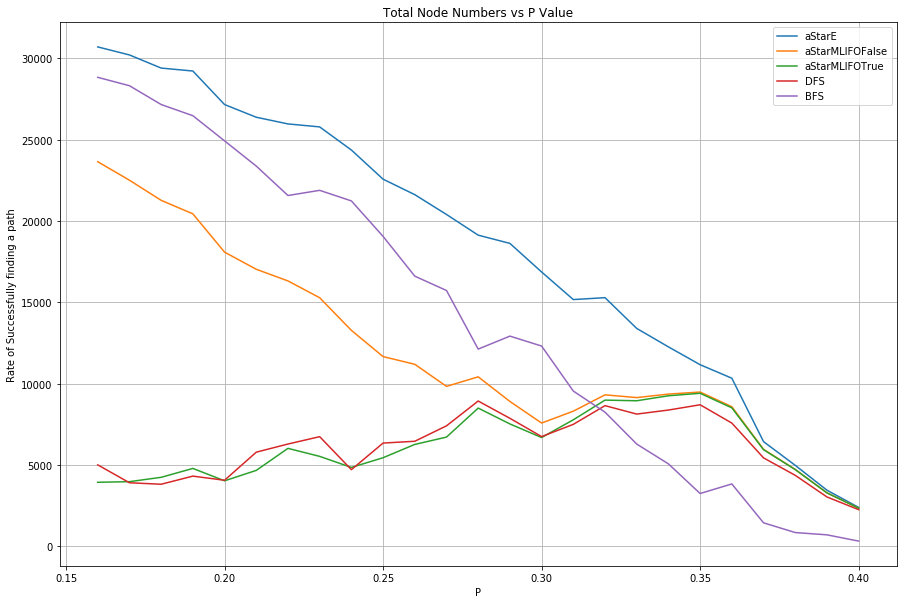
\includegraphics[width=\textwidth]{../pics/question7-3.png}
		\caption{\label{fig:7-3} Comparison of average number of nodes expanded.}
	\end{figure}
	
	
\end{questions}

\begin{bonus}
	\item {Why were you not asked to implement UFCS?} \\
	UFCS is equal to $ A^* $ algorithm with a heuristic function that always returns 0. In this mazerunner case, the cost of all steps are 1, so UFCS is exactly equal to BFS.
\end{bonus}

\section{Part 2: Building Hard Mazes}
	\label{sec:Part 2: Building Hard Mazes}
	\begin{enumerate}[resume]
		
		\item {What local search algorithm did you pick, and why? How are you representing the maze/environment, to be able to utilize your chosen search algorithm? What design choices did you have to make to apply this search algorithm to this problem?}
		
		\begin{enumerate}
			\item {What local search algorithm did you pick, and why?} \\
			We combined Genetic Algorithm with Simulated-Annealing-Based Beam Search. We have several reasons: \\
			\begin{enumerate}
				\item {Genetic Algorithm works much better than Simulated-Annealing-Based Beam Search when the mutation rate is large.} \\
				
				\item {Genetic Algorithm usually returns mazes with the "pattern"(or say "schema") that makes a maze hard. However, it is hard to finetune the "pattern" when its size is too large because the pattern is likely to be cut into 2 halves and unlikely to be pieced together again. For instance, (one of) the ideal pattern of the longest path maze should seem like a Hilbert curve, which is as large as the maze. A slight dislocation will make the maze unsolvable. Hence we need another algorithm to finetune.} \\
				
				\item {Beam Search requires a brunch of initial states(mazes), which perfectly matches the population of final iteration from Genetic Algorithm. Also, Simulated Annealing can be helpful when it runs into a local maximum. Combine Beam Search and Simulated Annealing to both utilize most mazes that Genetic Algorithm returned and avoid converging at a local maximum.}
			\end{enumerate}
			
			\item {How are you representing the maze/environment, to be able to utilize your chosen search algorithm? What design choices did you have to make to apply this search algorithm to this problem?} 
			
			\textbf{Overall:}
			\begin{enumerate}
				\item {A maze can be represented by a $ rows \times cols $ boolean matrix, where True means this block is a wall, and False means the agent can go through this block.} \\
				
				\item {The objective function value(fitness) of a maze is calculated by this formula: $$ObjectiveFunction(maze) = 
					\begin{bmatrix}
						BlockCount & PathLength & FringeSize \\
					\end{bmatrix} 
					\times 
					\begin{bmatrix}
						w_{block} \\
						w_{path}\\
						w_{fringe} 
					\end{bmatrix}$$  If we want to find the hardest maze in terms of a single aspect, set one weight to 1, and set others to 0.} \\
				
				\item {Genetic Algorithm will return much more mazes than what Beam Annealing requires. Therefore, using the idea similar to Simulated Annealing to pick some mazes as seeds of Beam Annealing.} \\
				\begin{enumerate}
					\item {Pick a few best mazes as "perfect seeds".} \\
					
					\item {Discard mazes whose fitness is lower than some percent, say 90\%, of maximum fitness, if the number of remained mazes is larger than the size of Beam Search.} \\
					
					\item {Randomly pick some "non-prefect seeds" with the probability: $$P = e^{{\frac{Weight}{PerfectRatio}+Bias}}, PrefectRatio = \frac{ObjectiveFunction(otherMaze)}{ObjectiveFunction(bestMaze)}$$} \\
					
					\item {Keep picking until the number of "seeds" equals the size of Beam Search.}
				\end{enumerate}
			
				\item {After Beam Annealing, compare the fine-tuned result with previous Genetic Algorithm's result. Return best several mazes of both results. (In this case, Beam Annealing failed because Genetic Algorithm presented a nearly perfect result. However, Annealing allows mazes to get a little easier, which is difficult to become harder again since it is hard to randomly get a perfect maze.} 
			\end{enumerate} 
		
			\textbf{Genetic Algorithm:} \\
			TODO \\
			
			\textbf{Beam Annealing:} \\
			\begin{enumerate}
				\item {A maze's neighbors are all the mazes that can become this maze by changing several blocks. Therefore, we choose a very small probability to flip each block's value to generate some neighbors of this maze for Stochastic Beam Search.} \\
				
				\item {Each solution algorithm returns 3 values: the number of blocks it has explored, the length of the path found, and the maximum size of the fringe it has used.} \\
				
				\item {The probability to move down is calculated by this formula: $$P = e^{\frac{Weight*\Delta E+Bias}{Temperature}}, \Delta E = ObjectiveFunction(newMaze) - ObjectiveFunction(maze)$$ A larger $Weight$ can decrease $P$ without any other influence. A larger $Bias$ mainly decrease the probability to keep step forward and back in a "plateaux", which works together with "impatient halt"(explained in Question 9).} \\
				
				\item {Decrease the temperature by multiply a const smaller than 1.0, called "cool rate", which makes the temperature go down fast at first and then getting slower and slower to let agent have more chance to climb up(explained in Question 9).} \\
				
				\item {Speaking of Beam Annealing, the key point is to make an agent can "regress" to where it was, especially when an agent "teleports" to another agent's region. Hence, once an agent teleport, one of its neighbors is set to a maze in the previous region.} \\
				
				\item {In order to increase the performance, each neighbor maze will be check if it is solvable by using BDA*. If it is unsolvable, regenerate it.}
			\end{enumerate}
		\end{enumerate}
		
		\item {Unlike the problem of solving a maze, for which the ‘goal’ is well-defined, it is difficult to know when we have constructed the ‘hardest’ maze. That being so, what kind of termination conditions can you apply to your search algorithm to generate ‘hard’ if not the ‘hardest’ mazes? What kind of shortcomings or advantages do you anticipate your approach having?} \\
		
		\textbf{Genetic Algorithm:} \\
		TODO\\
		
		\textbf{Beam Annealing:} \\
		There are 3 different ways to halt the iteration: \\
		\begin{enumerate}
			\item {Maximum Iteration Limit: Count the time it iterates. Once it exceeds the limit, halt and return the result.} 
			\begin{itemize}
				\item {It is the easiest way to terminate iteration, but actually, there is no reason to terminate it EXACTLY there, except that it has run too many times.}
			\end{itemize}
		
			\item {System Cooled Down: As time goes(it iterates), the temperature of Annealing decreases. If it is below a minimum temperature, halt and return the result.} 
			\begin{itemize}
				\item {If the temperature is too "cold", there is no need to keep Annealing. No easier mazes could be picked up. It is reasonable.}
				\item {It related to the cool rate. If the cool rate is too small, the temperature will decrease too fast, and there is not enough time for a maze getting harder after becoming easy. However, if the cool rate is too large, the temperature will keep a high level for a long time, which may totally destroy the work Genetic Algorithm has done.}
			\end{itemize}
		
			\item {No Patience Left: If agents do not move for a really long time, it must converge at a local optimal. It is time to halt and return the result.} 
			\begin{itemize}
				\item {Since we have found a local optimal, we should return it.}
				\item {In the beginning, it is less likely to converge. Hence we should iterate it for a little more times. But if it has been iterated for lots of times, it is unnecessary to keep iterations going.}
				\item {When an agent climbs on a "plateaux", it will get lost. Hence, we should limit its ability to move to an equal-difficult maze by using $Bias$ to calculate the probability to move.}
				\item {The issue is, sometimes, Genetic Algorithm returns a "nearly perfect" maze. In this case, it takes at least 30 iterations to halt, since we assume what Genetic Algorithm did is just pre-training.}
			\end{itemize}
		\end{enumerate}
		
		\item {For each of the following algorithms, do the following: Using your local search algorithm, for each of the following properties indicated, generate and present three mazes that attempt to maximize the indicated property. Do you see any patterns or trends? How can you account for them? What can you hypothesize about the ‘hardest’ maze, and how close do you think you got to it?}
		\begin{enumerate}
			\item {DFS} \\
			\label{DFS}
			The configuration of DFS is set to 'quickGoal' : True, 'distinctFringe' : True, and all others are False.
			\begin{enumerate}
				\item {Length of solution path returned: See Figure \ref{fig:dp1}, Figure \ref{fig:dp2} and Figure \ref{fig:dp3}.} \\
				\begin{figure}
					\minipage{\textwidth}
					
						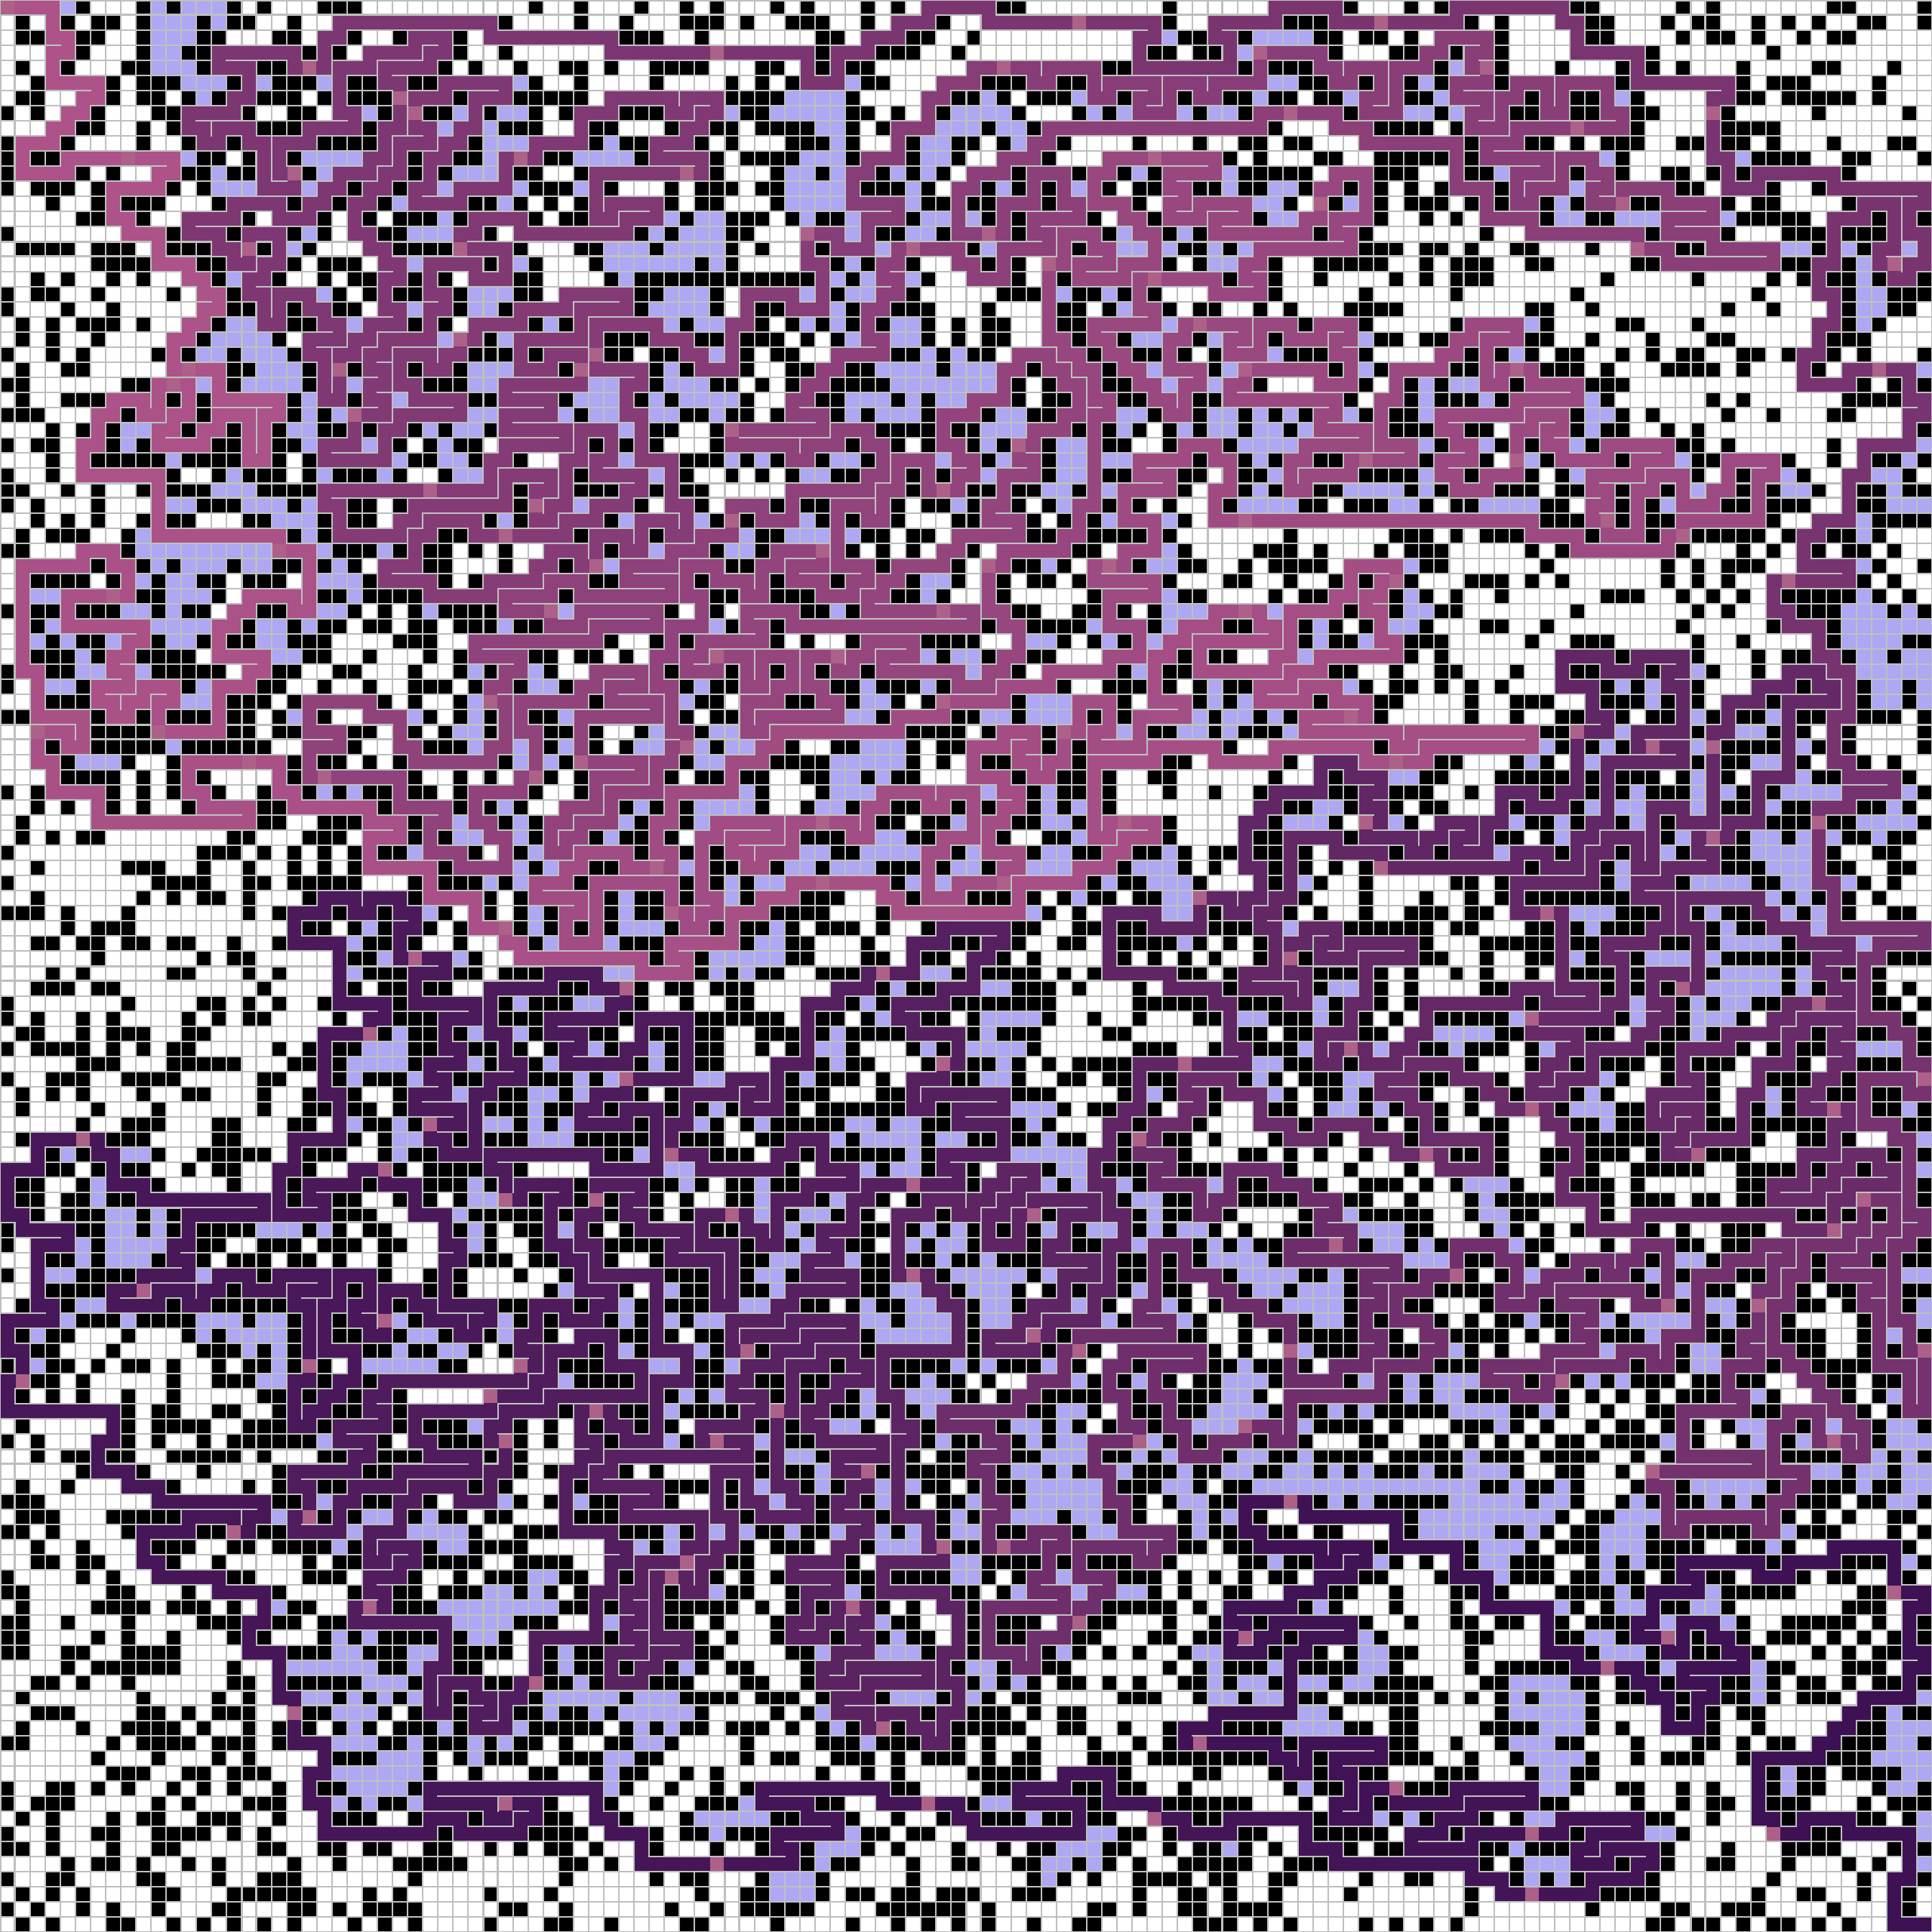
\includegraphics[width=\textwidth]{../pics/dp/5557.png}
						\caption{\label{fig:dp1}maze that is hard for DFS in terms of path length, which is 5557.}
						
						\minipage{0.49\textwidth}
							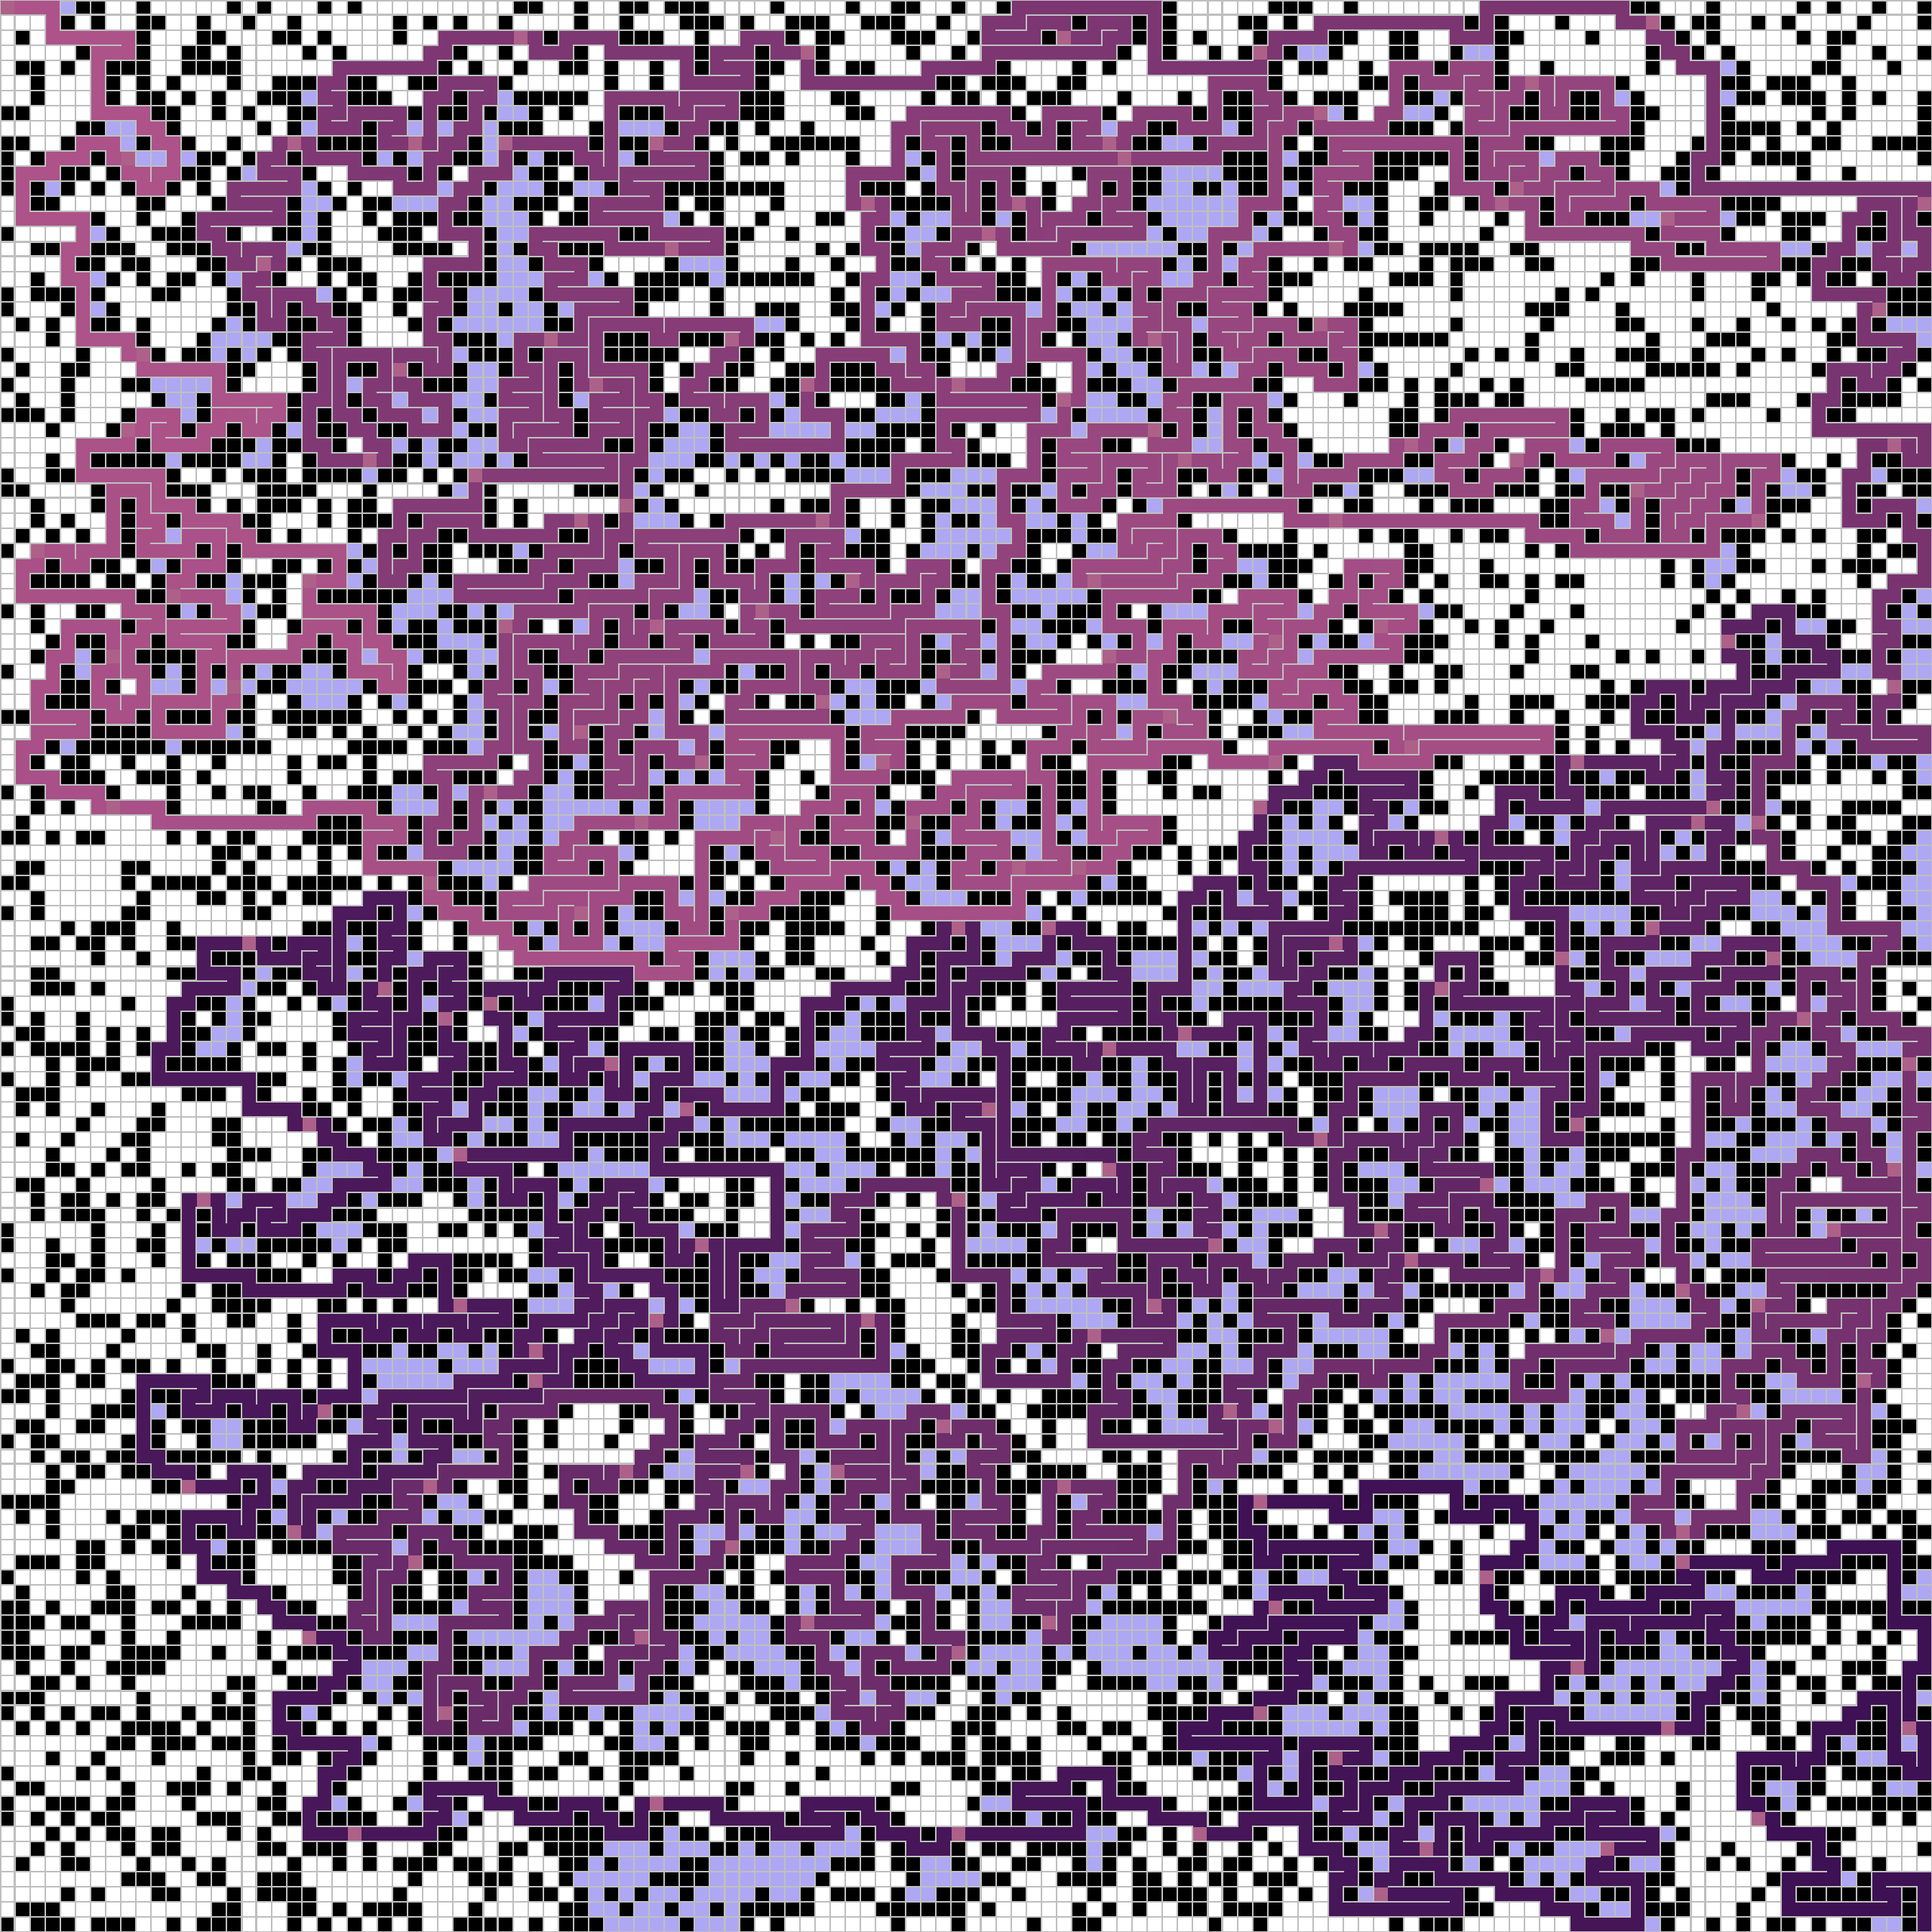
\includegraphics[width=\textwidth]{../pics/dp/5503.png}
							\caption{\label{fig:dp2}maze that is hard for DFS in terms of path length, which is 5503.}
						\endminipage\hfill
						\minipage{0.49\textwidth}
							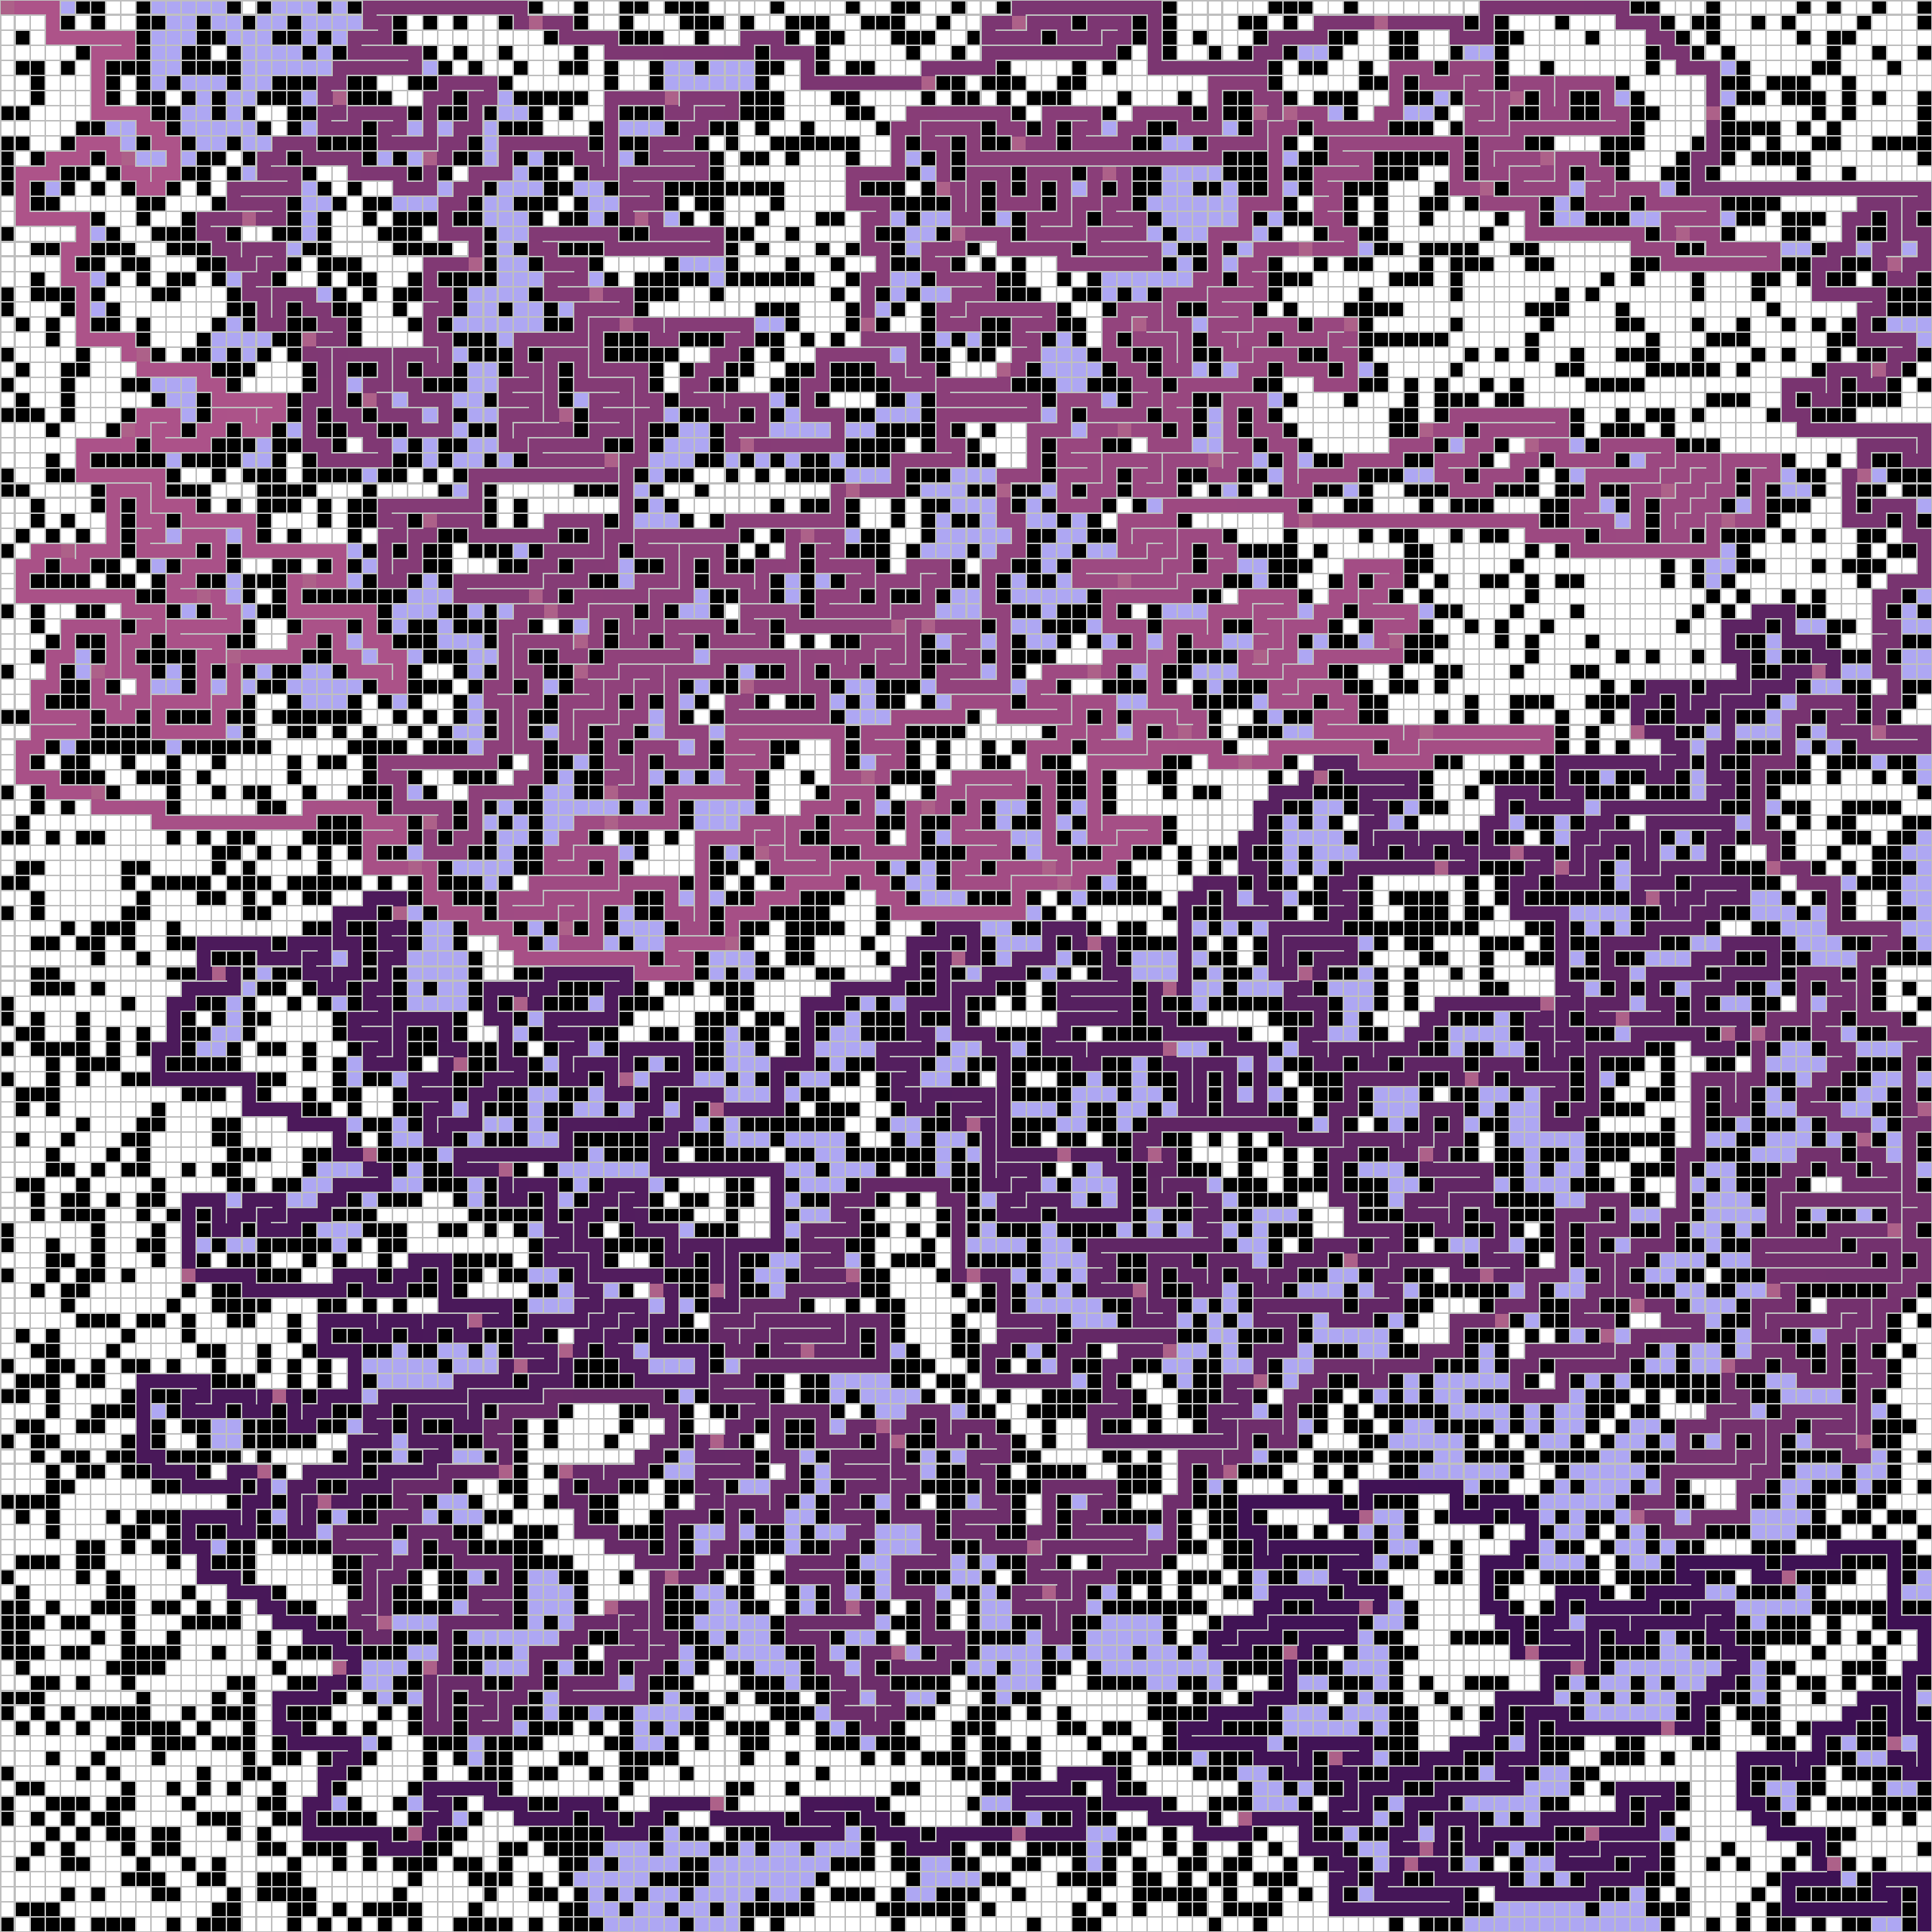
\includegraphics[width=\textwidth]{../pics/dp/5495.png}
							\caption{\label{fig:dp3}maze that is hard for DFS in terms of path length, which is 5495.}
						\endminipage
					\endminipage
					
				\end{figure}
				\textbf{Patterns or trends:} 
				\begin{itemize}
					\item {There are 2 classical patterns of walls. (See Figure \ref{fig:dp-pattern}) In one case, walls lead agents to go down some rows, then there usually several nearly "empty"(no walls) rows to move horizontally. But at the end of these rows, diagonal walls lead agents to move up. This case looks like "I" and ">". The other case is "J-shape" walls. }
					\begin{figure}
						\minipage{0.6\textwidth}
							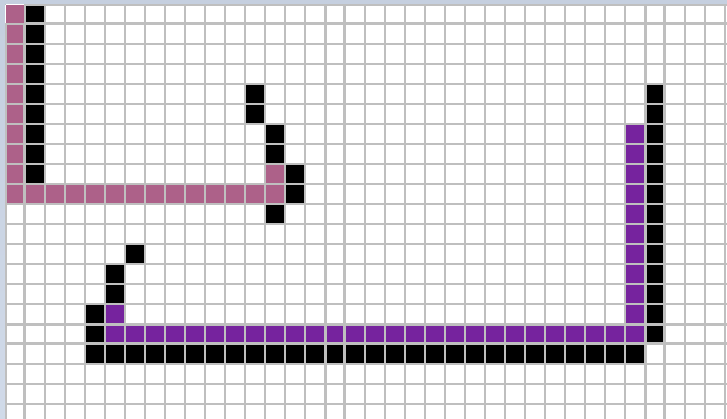
\includegraphics[width=\textwidth]{../pics/dp/pattern.png}
							\caption{\label{fig:dp-pattern}Two classical patterns of walls: "I" and ">" walls and "J-shape" walls.}
						\endminipage\hfill
						\minipage{0.39\textwidth}
							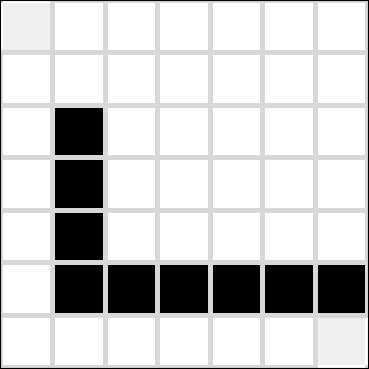
\includegraphics[width=\textwidth]{../pics/dp/hardest.png}
							\caption{\label{fig:dp-hardest}}
						\endminipage
					\end{figure}
				
					\item {"I" and ">" walls and "J-shape" walls appear alternately.}
				\end{itemize}
			
				\textbf{Reasons:} 
				\begin{itemize}
					\item {The key point is when randomWalk == False, the priority of 4 directions is Right > Down > Left > Up.}
					\item {"I" and ">" walls lead agent walk horizontally, and the path it has walked becomes "new wall" because those blocks have been added into the closed set. Now it becomes a "J-shape" walls in the mirror.}
					\item {"J- shape" walls force agents search all blocks inside because agents prefer to go right or left than to move up.}
				\end{itemize}
				
				\textbf{"The hardest" maze:} 
				\begin{itemize}
					\item {The ideal "J-shape" walls can be maze-sized. (See Fig \ref{fig:dp-hardest}) In this case, the path length can be $size \times size - WallCost = 16312$. Notice that if size is an odd number, not all the accessible blocks are in the path. Specifically, only the first 3 blocks in the 2nd row are in the path. }
					\item {Compared with 16312, 5557 is not a big number. However, it is extremely impossible to randomly set all walls in a line.}
					\item {However, compared with less than 1000 block length in a 200 by 200 maze(from Question 5), 5557 in a 128 by 128 maze can be regarded as a "harder" maze, though it is not the "hardest" maze.}
				\end{itemize}
			
				\item {Total number of nodes expanded: See Figure \ref{fig:dp1}, Figure \ref{fig:dp2} and Figure \ref{fig:dp3}.} \\
				\begin{figure}
					\minipage{\textwidth}
					
					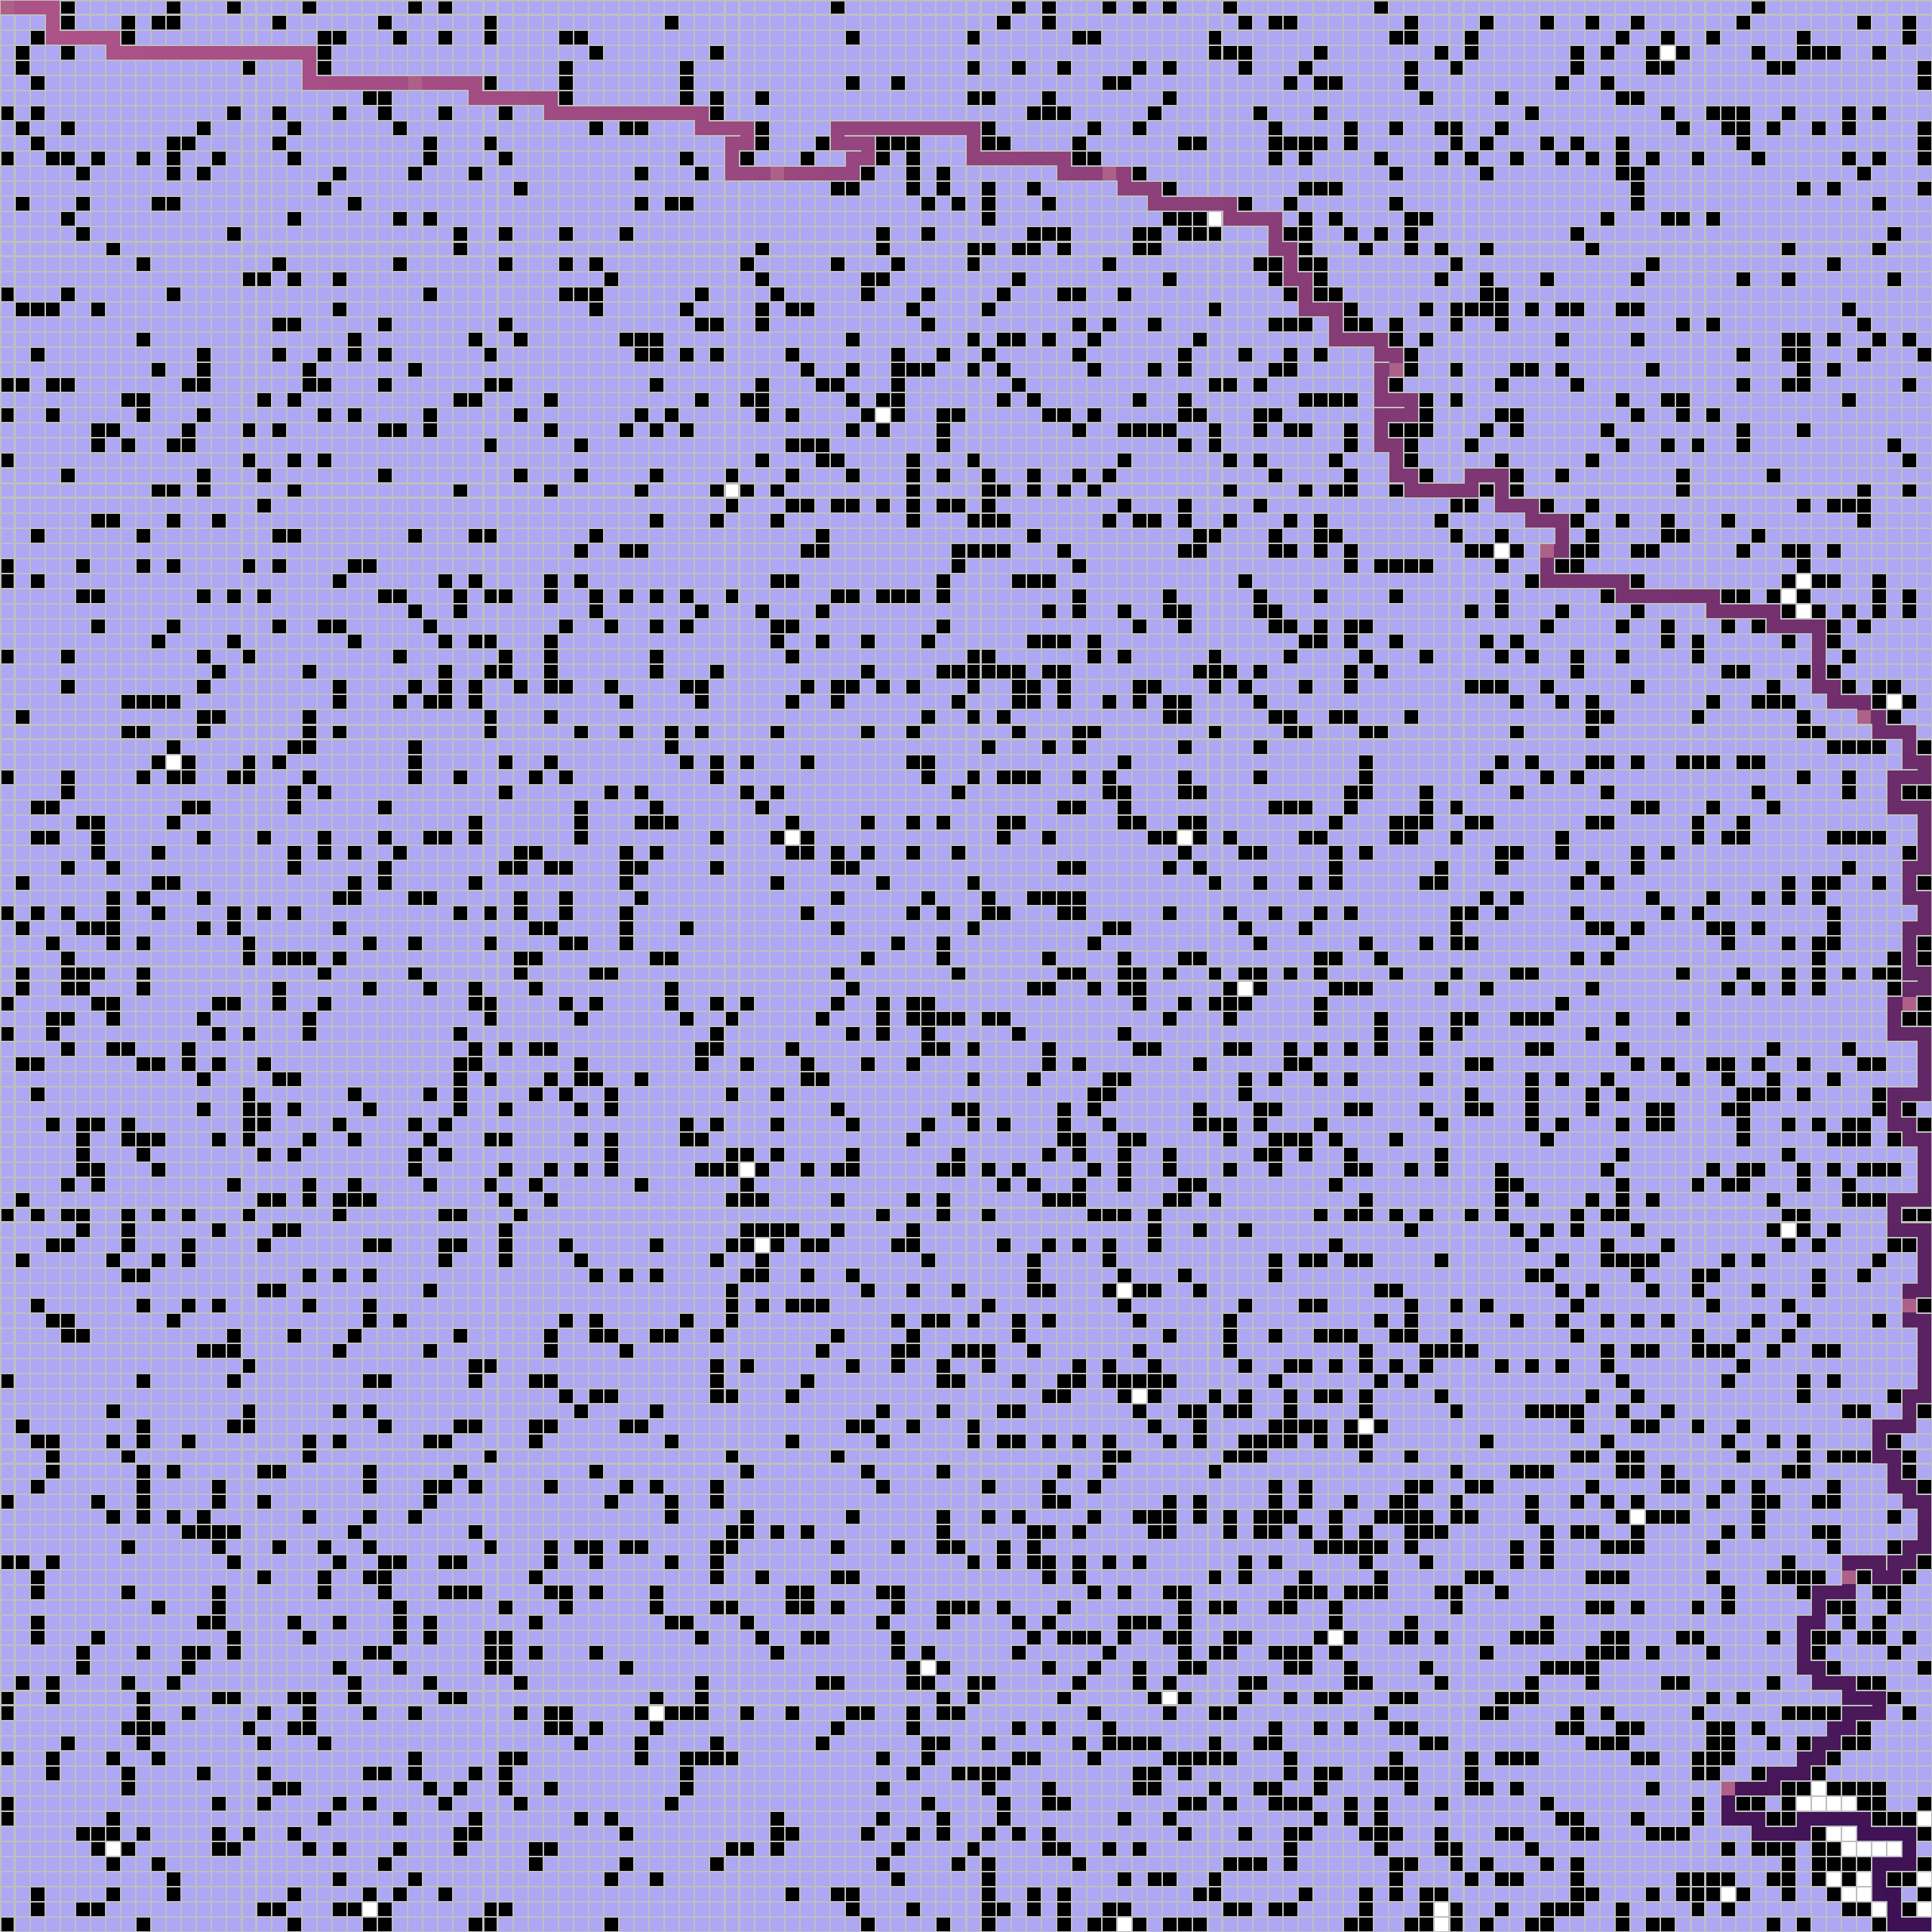
\includegraphics[width=\textwidth]{../pics/db/12993.png}
					\caption{\label{fig:db1}A maze that is hard for DFS in terms of time complexity, which has opend 12993 blocks.}
					
					\minipage{0.49\textwidth}
					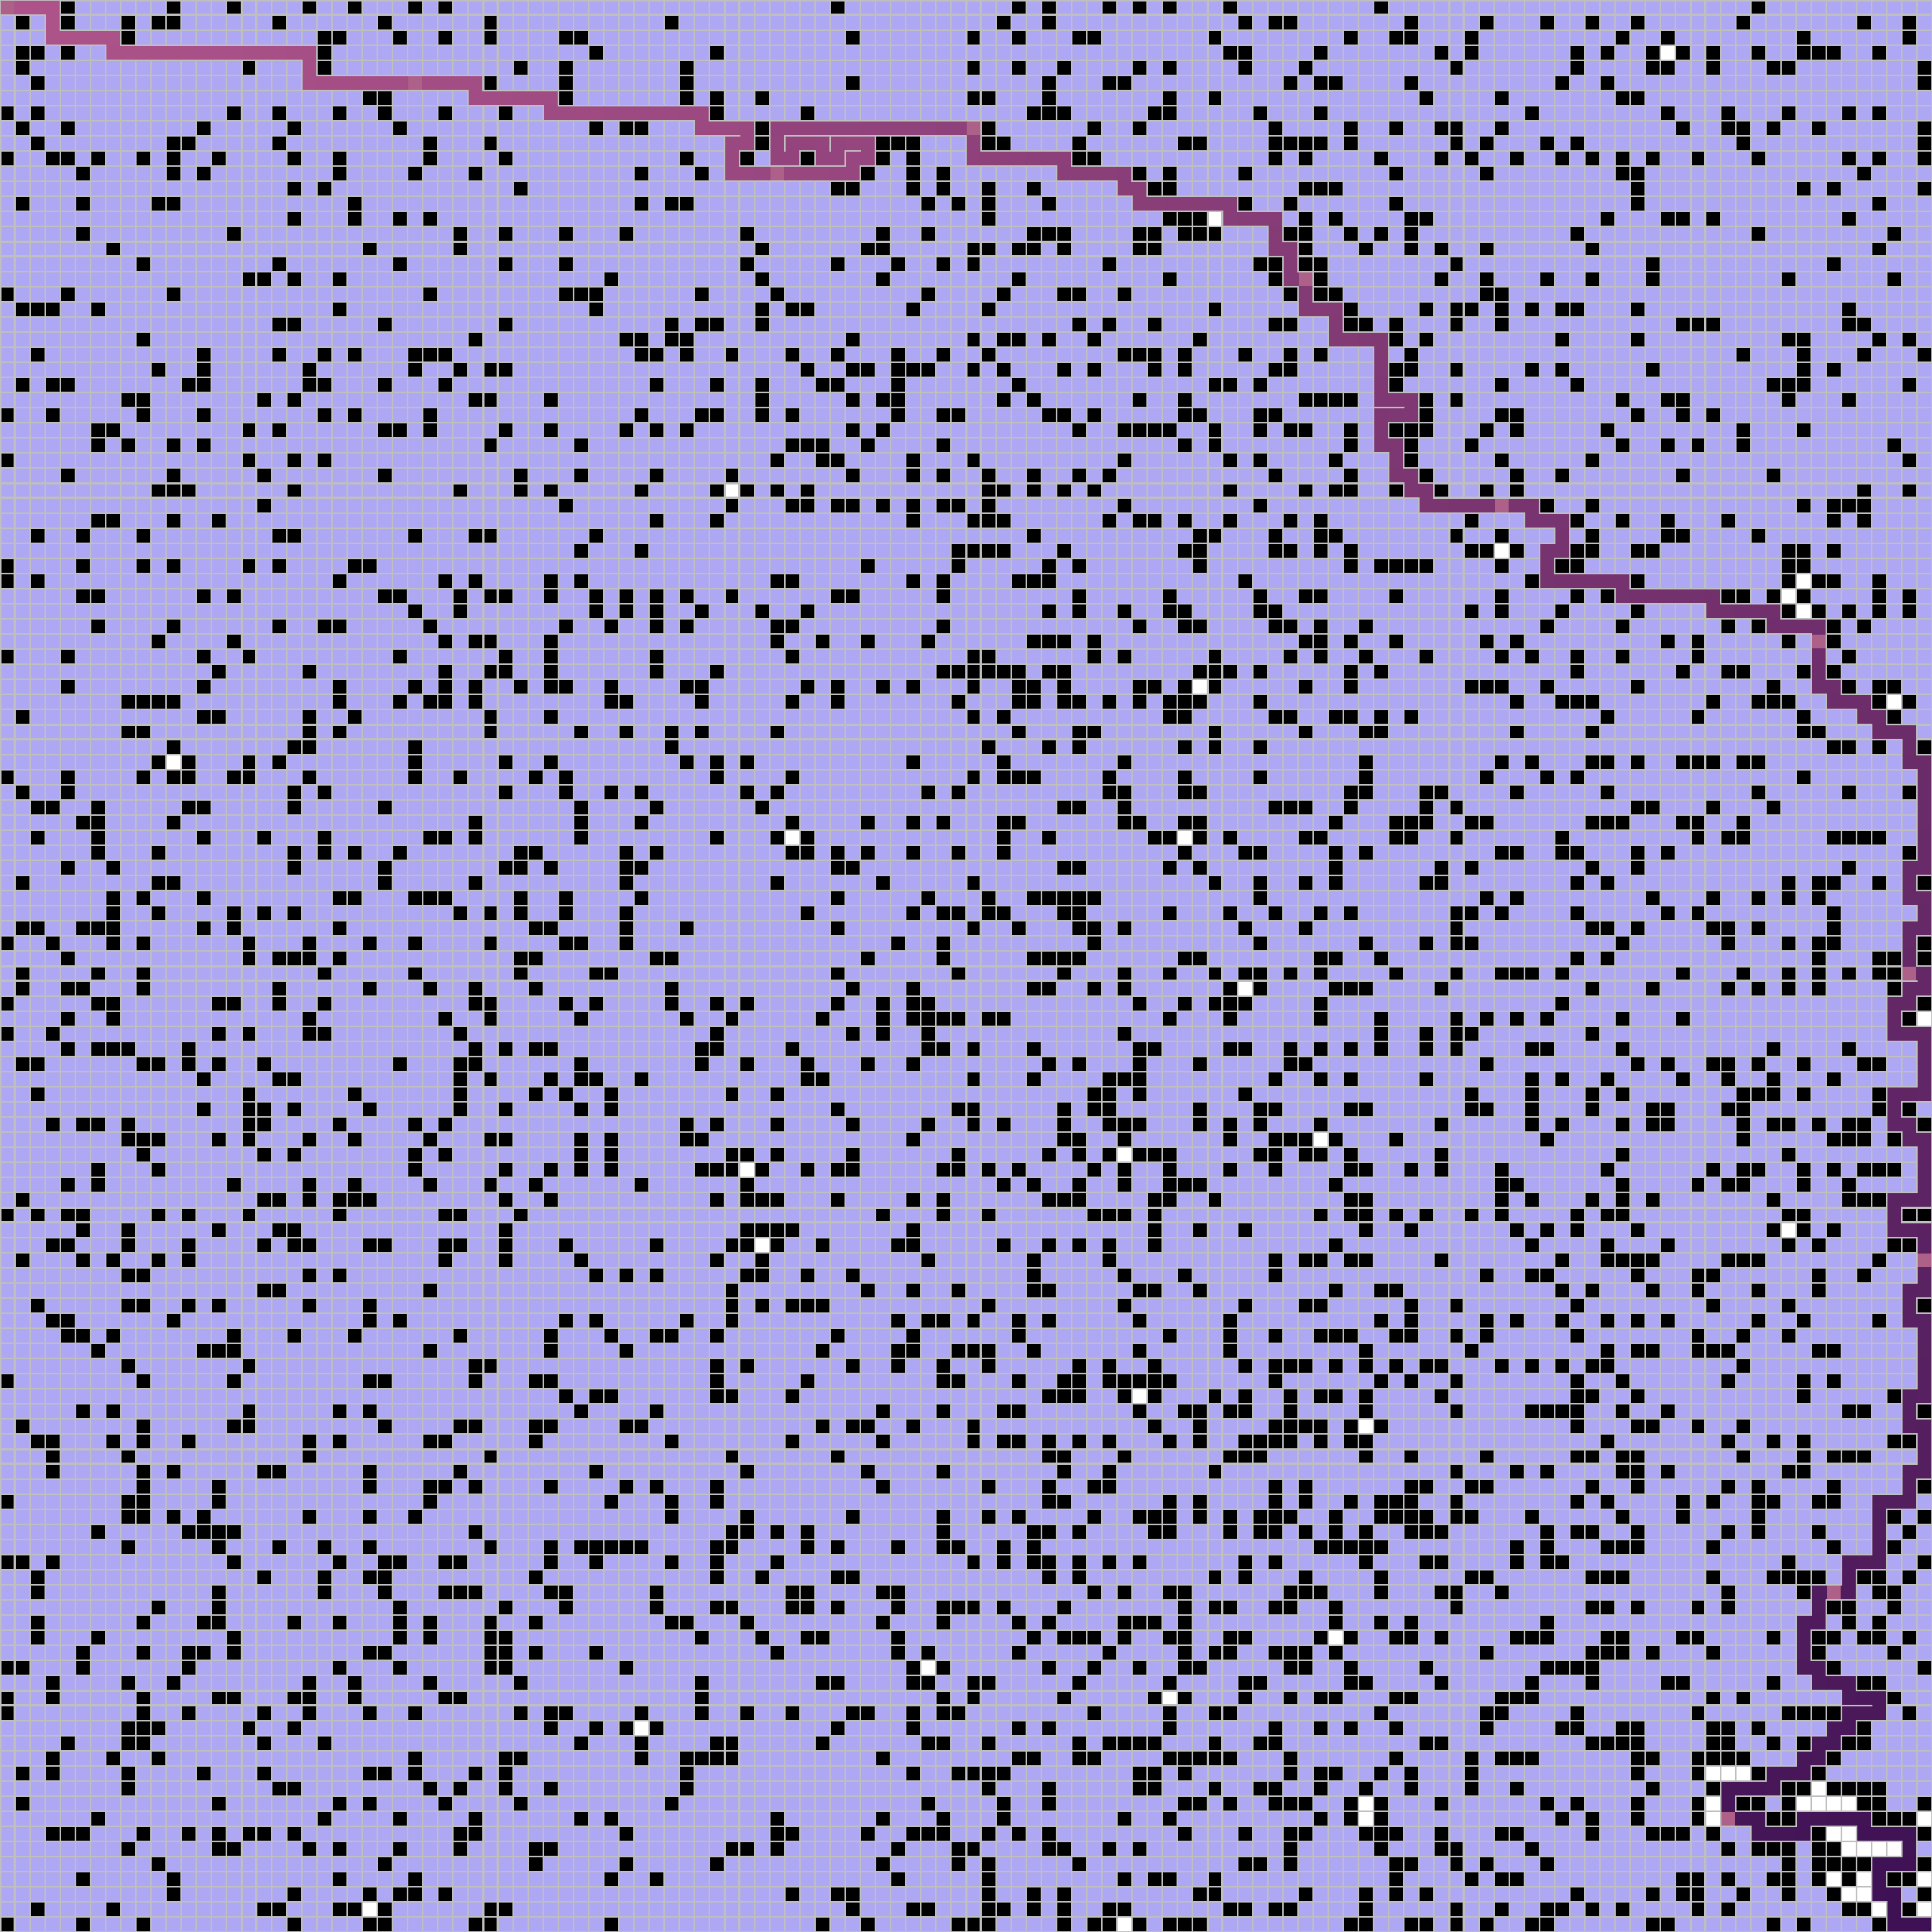
\includegraphics[width=\textwidth]{../pics/db/12968.png}
					\caption{\label{fig:db2}A maze that is hard for DFS in terms of time complexity, which has opend 12968 blocks.}
					\endminipage\hfill
					\minipage{0.49\textwidth}
					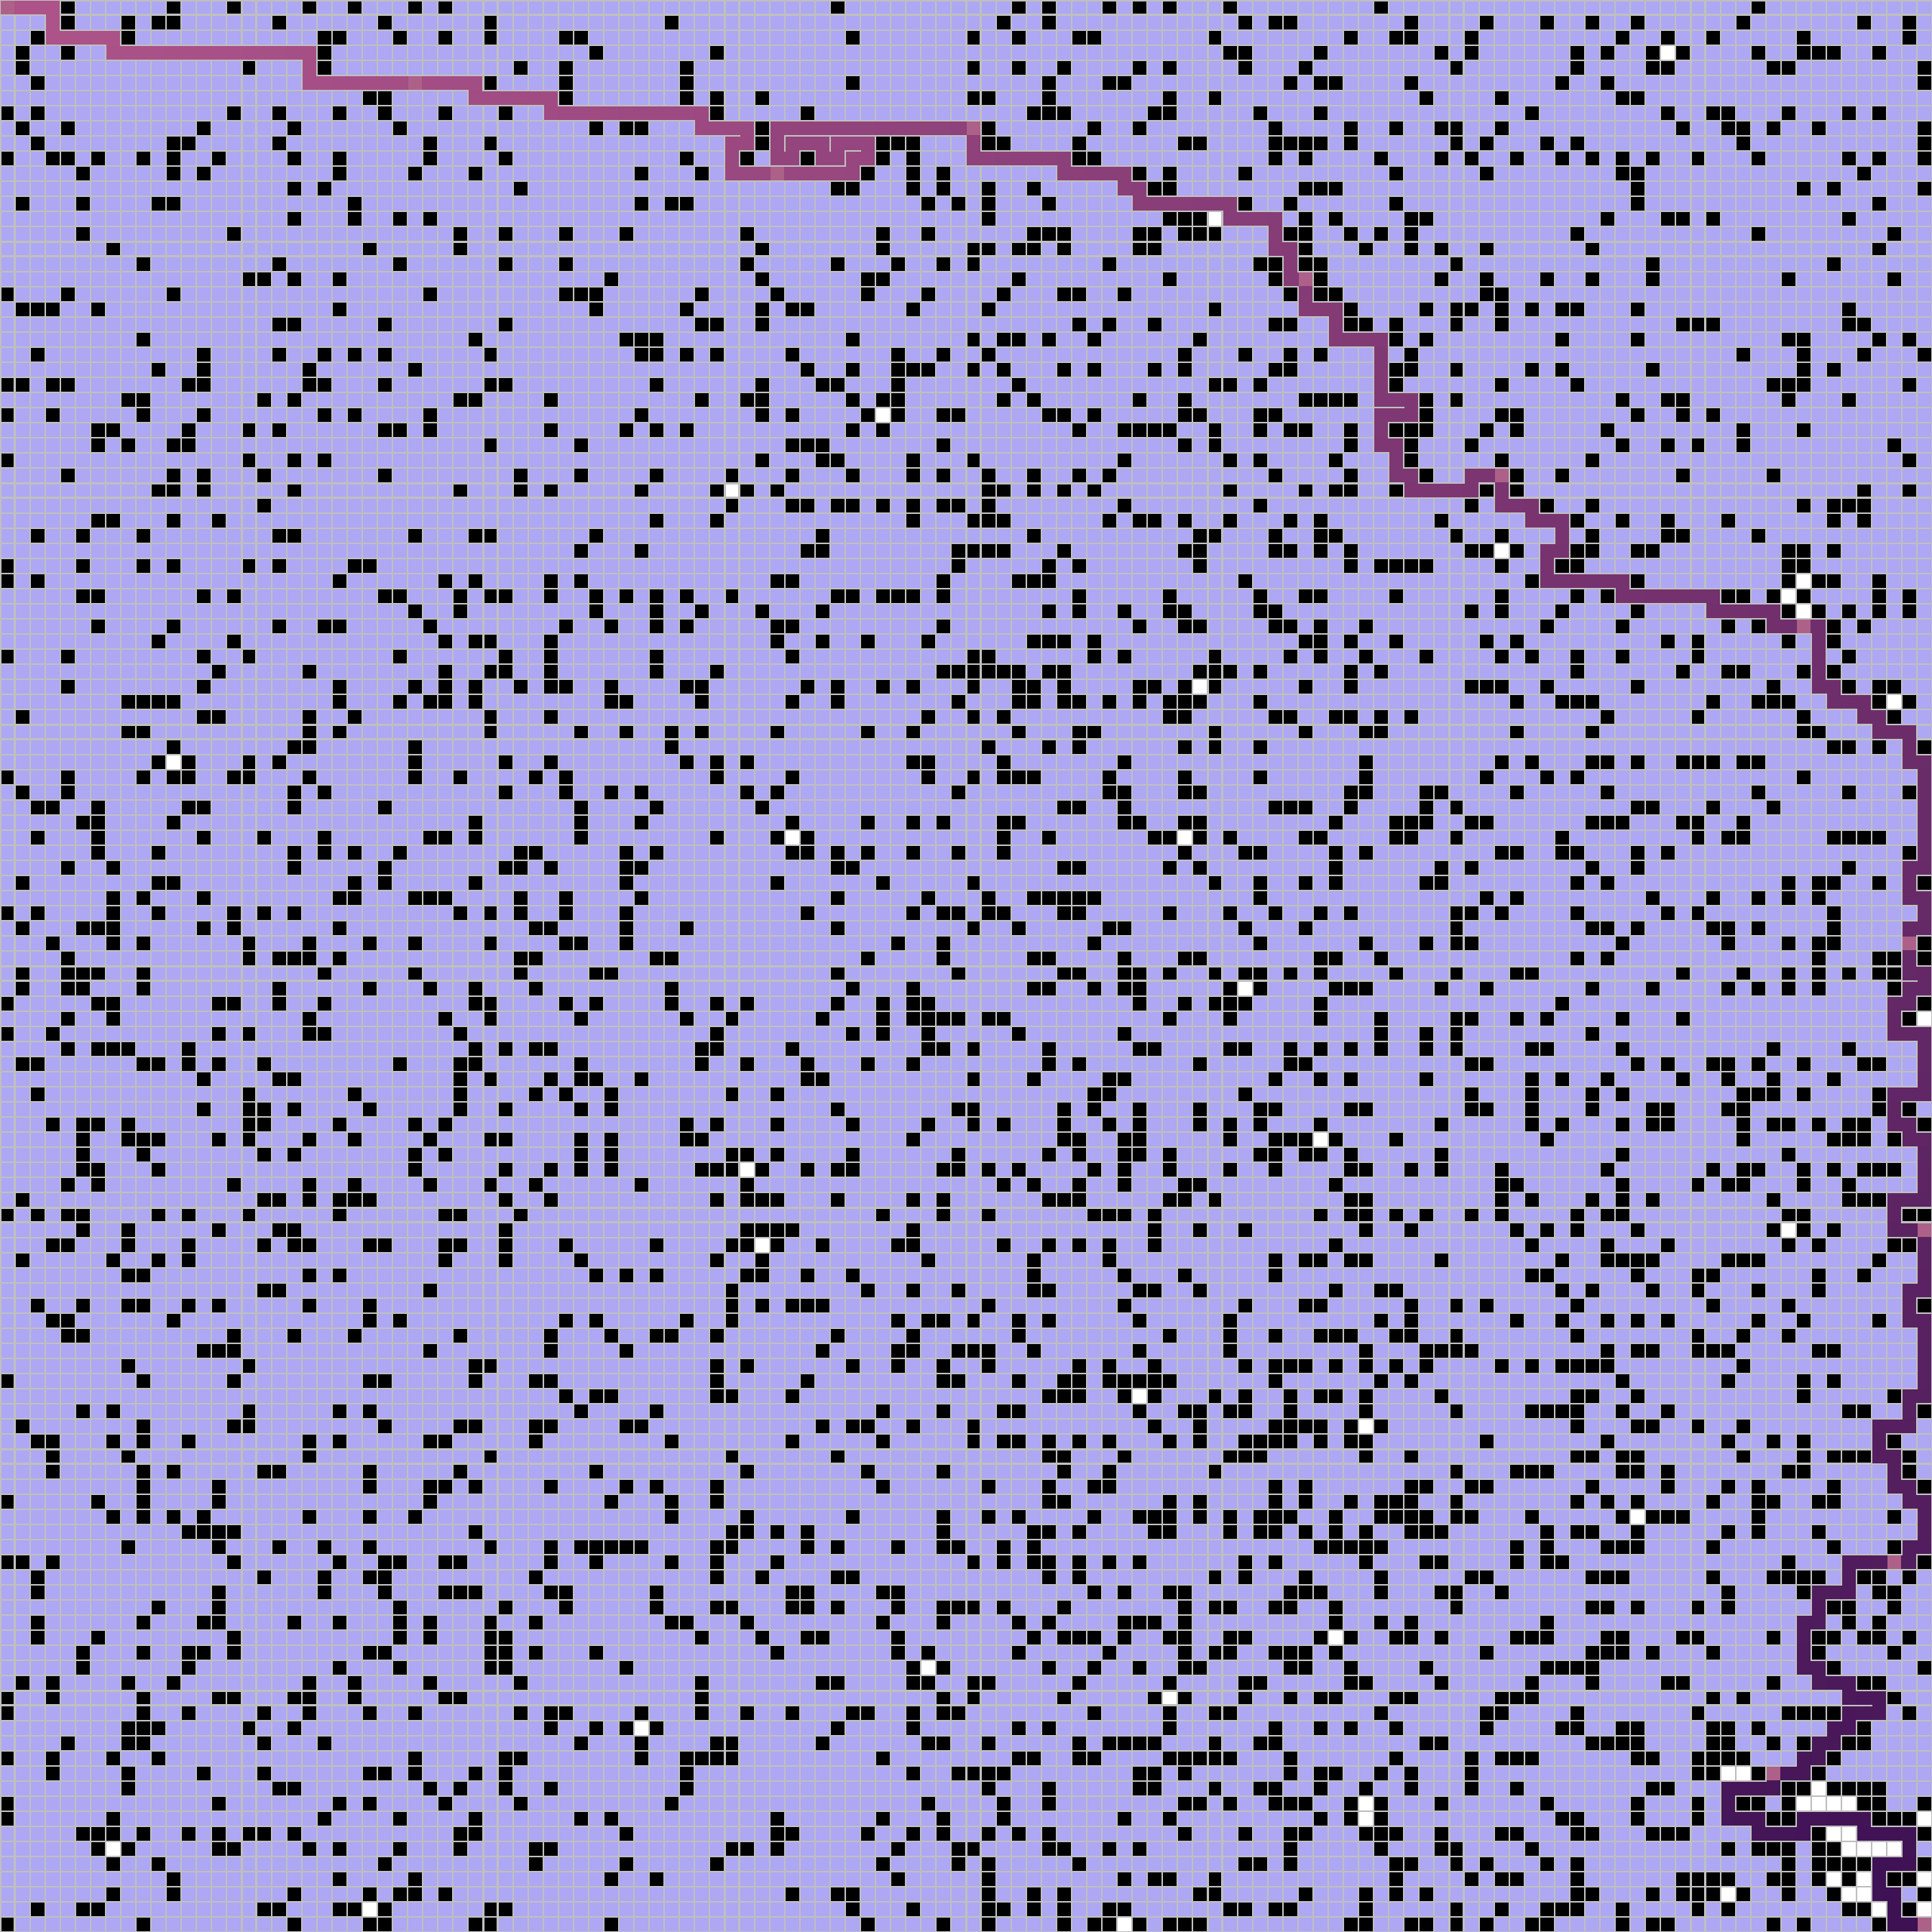
\includegraphics[width=\textwidth]{../pics/db/12967.png}
					\caption{\label{fig:db3} A maze that is hard for DFS in terms of time complexity, which has opend 12967 blocks.}
					\endminipage
					\endminipage 
				\end{figure}
			
				\textbf{Patterns or trends:} 
				\begin{itemize}
					\item {The pathway near the Goal(10 * 10 blocks in the lower right corner) is extremely narrow(only 1 block width), opens to left, and begins with a "door sill" wall that forces the path to move up a block.}
					
					\item {"I" and ">" walls and "J-shape" walls appear alternately.}
				\end{itemize}
				
				\textbf{Reasons:} 
				\begin{itemize}
					\item {Notice that when randomWalk == False, the priority of 4 directions is Right > Down > Left > Up.}
					\item {The pathway opens to left rather than up makes DFS cannot first run right to the last column and then find the pathway. It takes time for DFS to search all upper right part(above the path) and then realize "Oops, there is no way to the goal. I have to backtrack."}
					\item {After DFS reached the "door sill", it prefers to go to any directions but up. Hence, it takes more time for DFS to search all lower left part(below the path) and then realize "Alright, I will go up to see if there is a path."}
					\item {Therefore, DFS nearly searched all the blocks to reach the Goal.}
					\item {Notice that if randomWalk == True, this pattern will not always work because DFS may go down first rather than right.}
				\end{itemize}
				
				\textbf{"The hardest" maze:} 
				\begin{itemize}
					\item {A maze is "empty"(no walls) except the lower right corner. The lower right corner should be a pathway like this pattern. The smallest pattern can be done in 4 * 4.(See Fig \ref{fig:db-hardest}). Notice there must be at least 2 block height "door sill" for DFS to turn back to search lower left part. }
					\begin{figure}
						\centering
						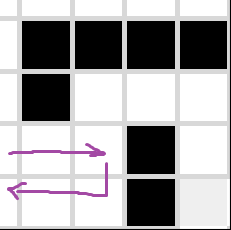
\includegraphics[width=0.3\textwidth]{../pics/db/hardest.png}
						\caption{\label{fig:db-hardest} The smallest pathway pattern.}
					\end{figure}
					\item {Compare to $size \times size - WallCost =16377$, 12993 can still be improved. However, it is really difficult to cancel out those outside walls by random without destroying the pattern. Therefore, it has been a nearly "hardest" maze.}
				\end{itemize}
			
				
				\item {Maximum size of fringe during runtime: See Figure \ref{fig:df1}, Figure \ref{fig:df2} and Figure \ref{fig:df3}.} \\
				\begin{figure}
					\minipage{\textwidth}
					
					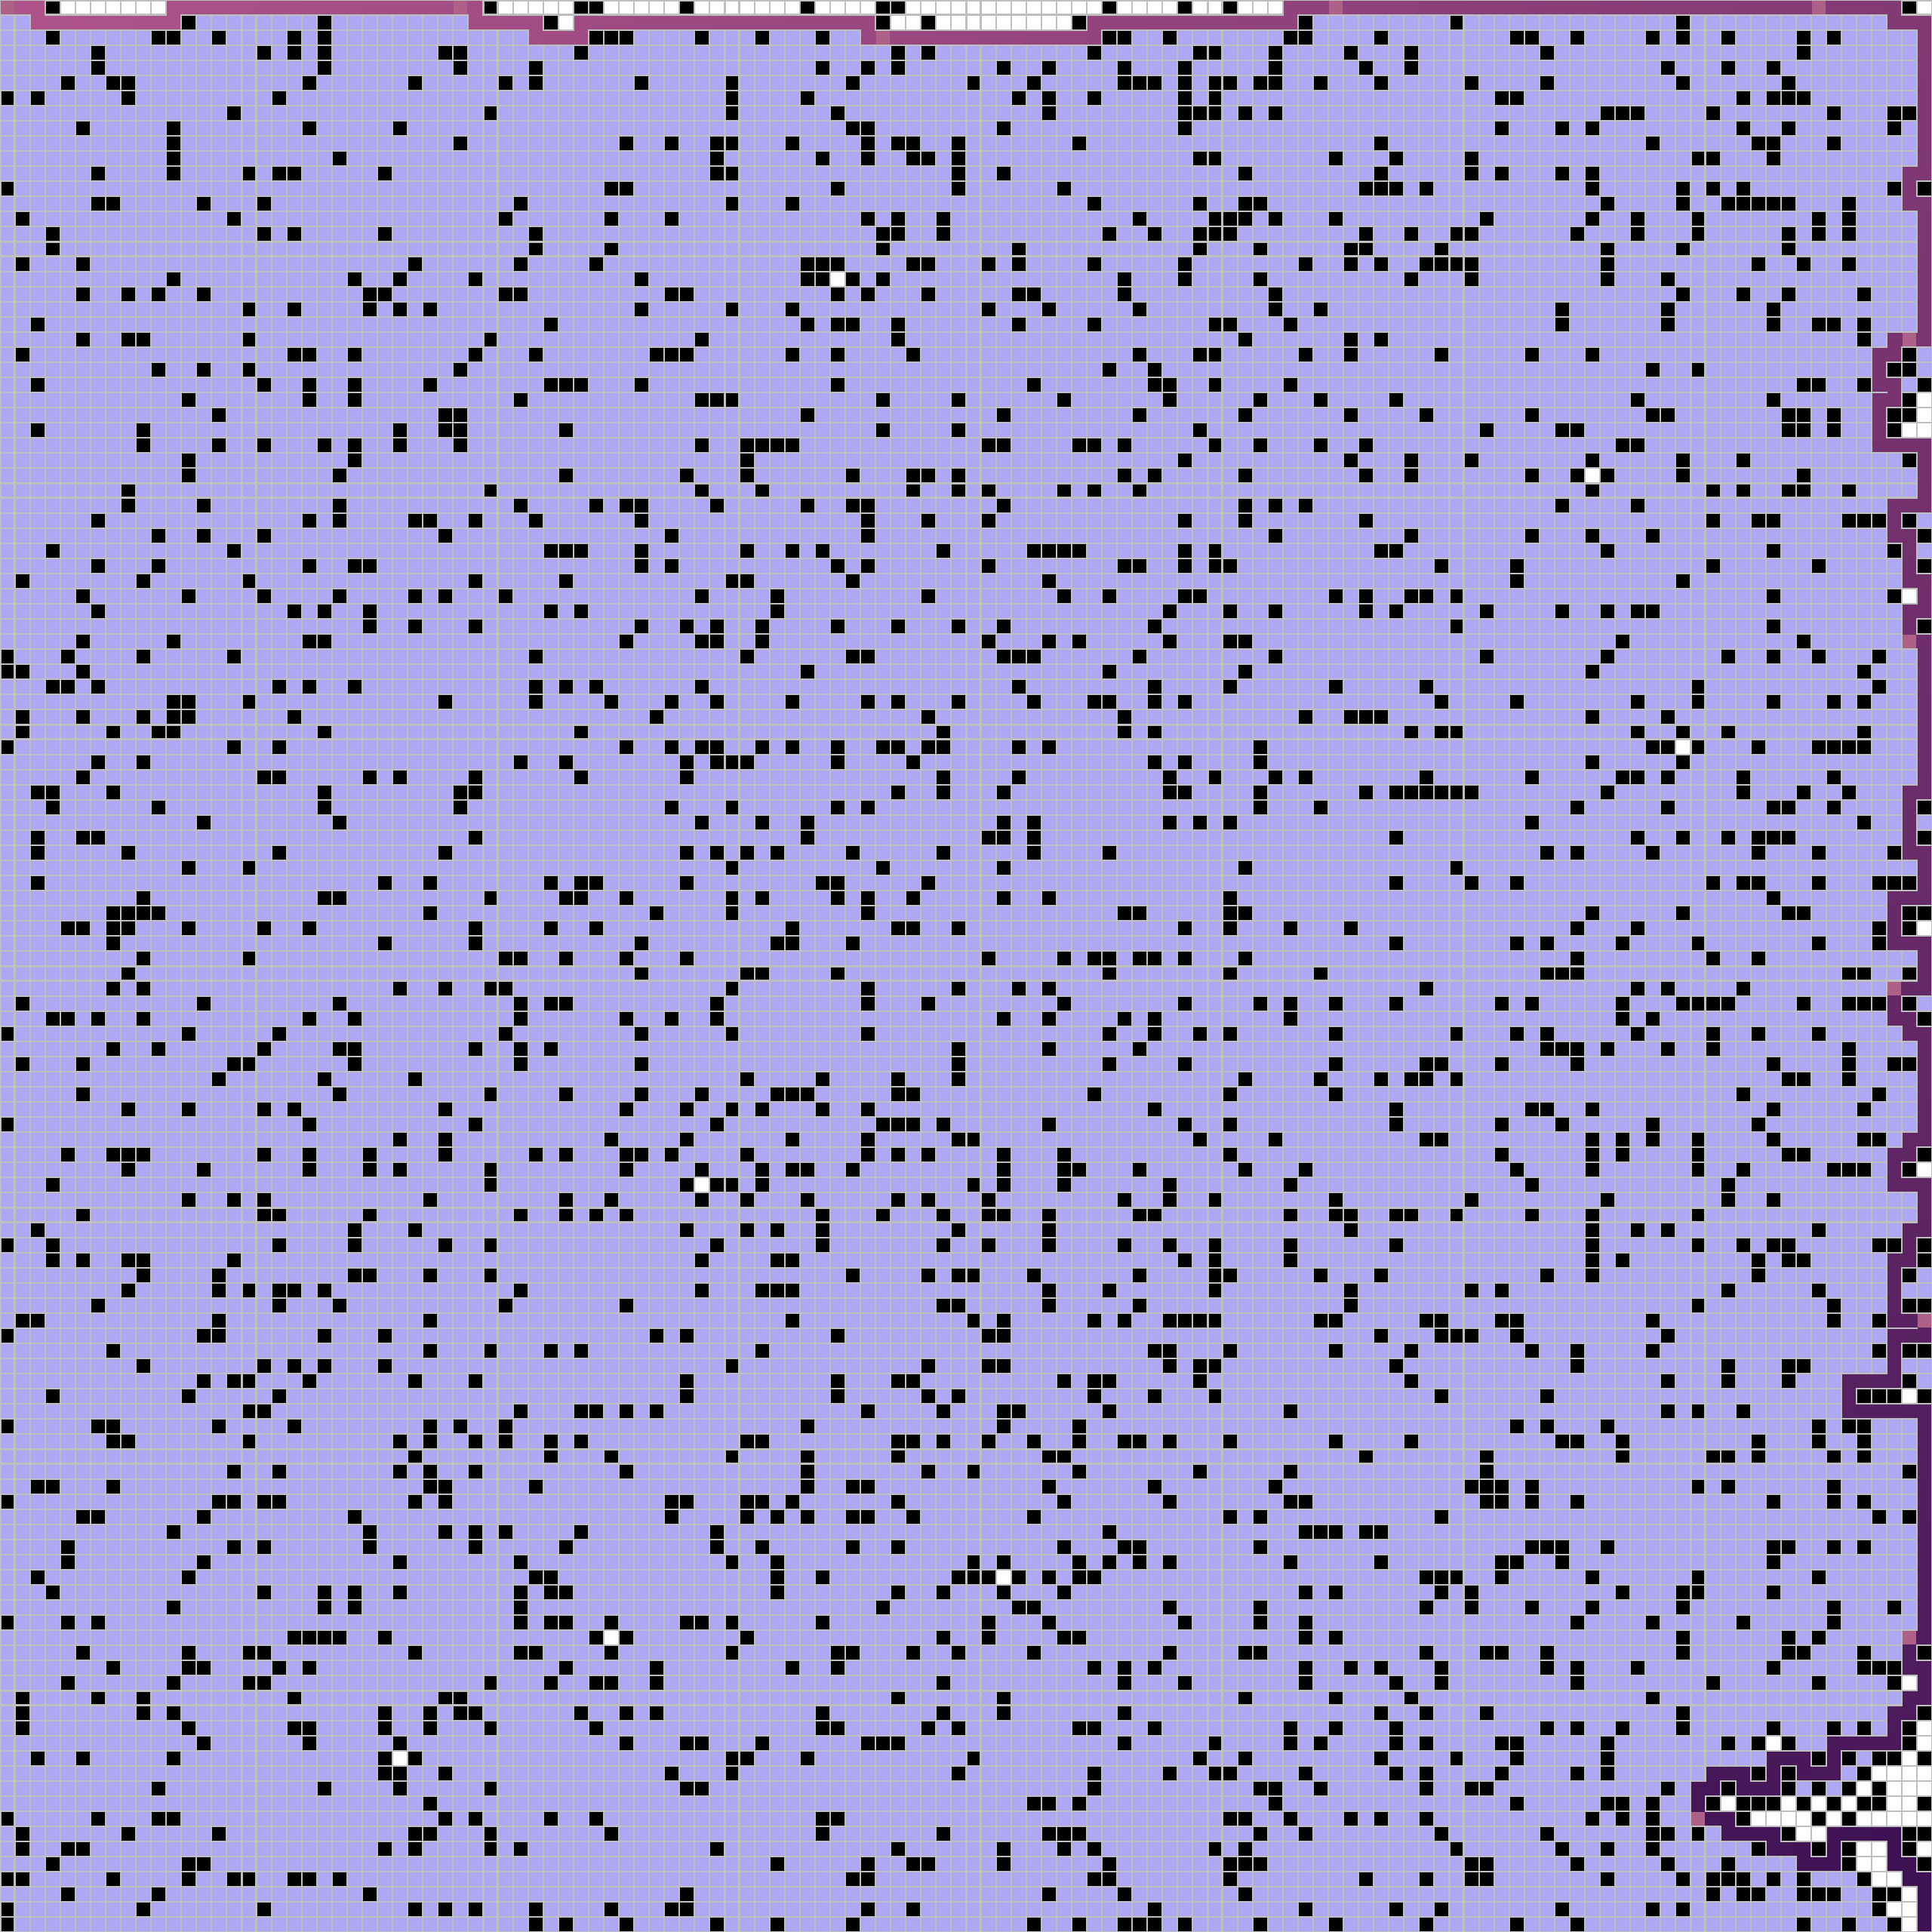
\includegraphics[width=\textwidth]{../pics/df/10032_2.png}
					\caption{\label{fig:df1}A maze that is hard for BFS in terms of space complexity, whose maximum fringe size is 10032. }
					
					\minipage{0.49\textwidth}
					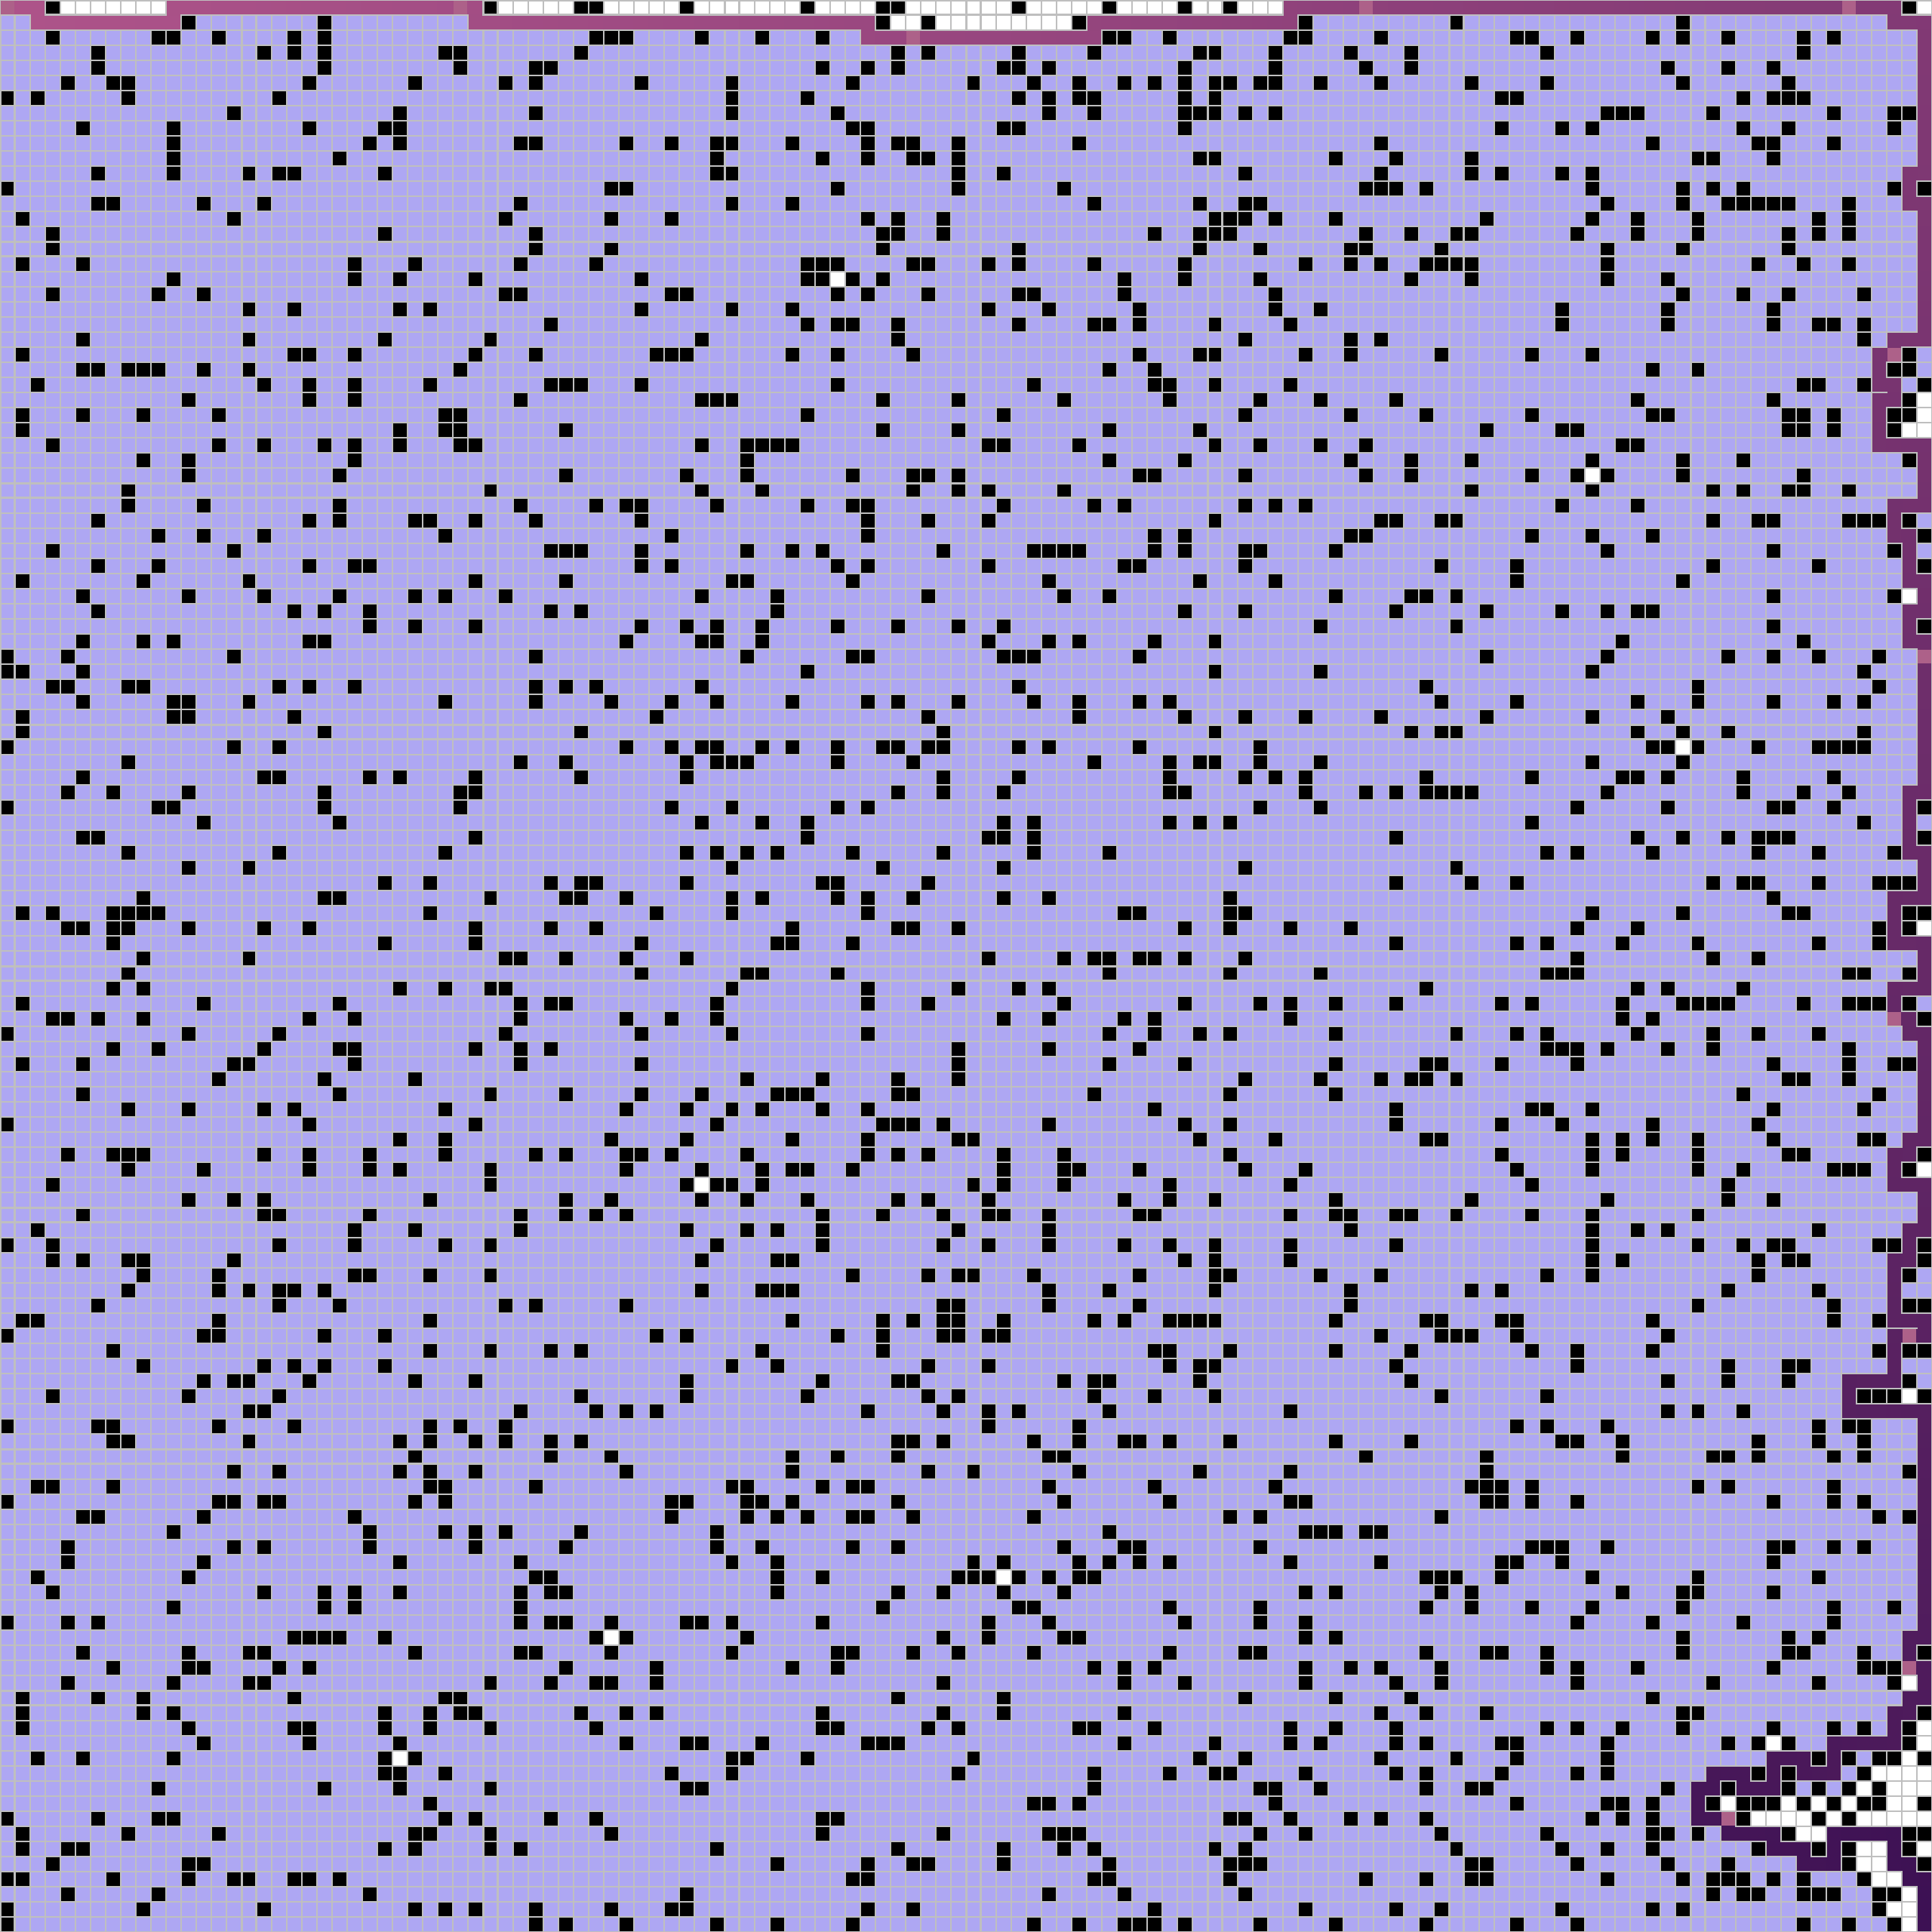
\includegraphics[width=\textwidth]{../pics/df/10032.png}
					\caption{\label{fig:df2}A maze that is hard for BFS in terms of space complexity, whose maximum fringe size is 10032. }
					\endminipage\hfill
					\minipage{0.49\textwidth}
					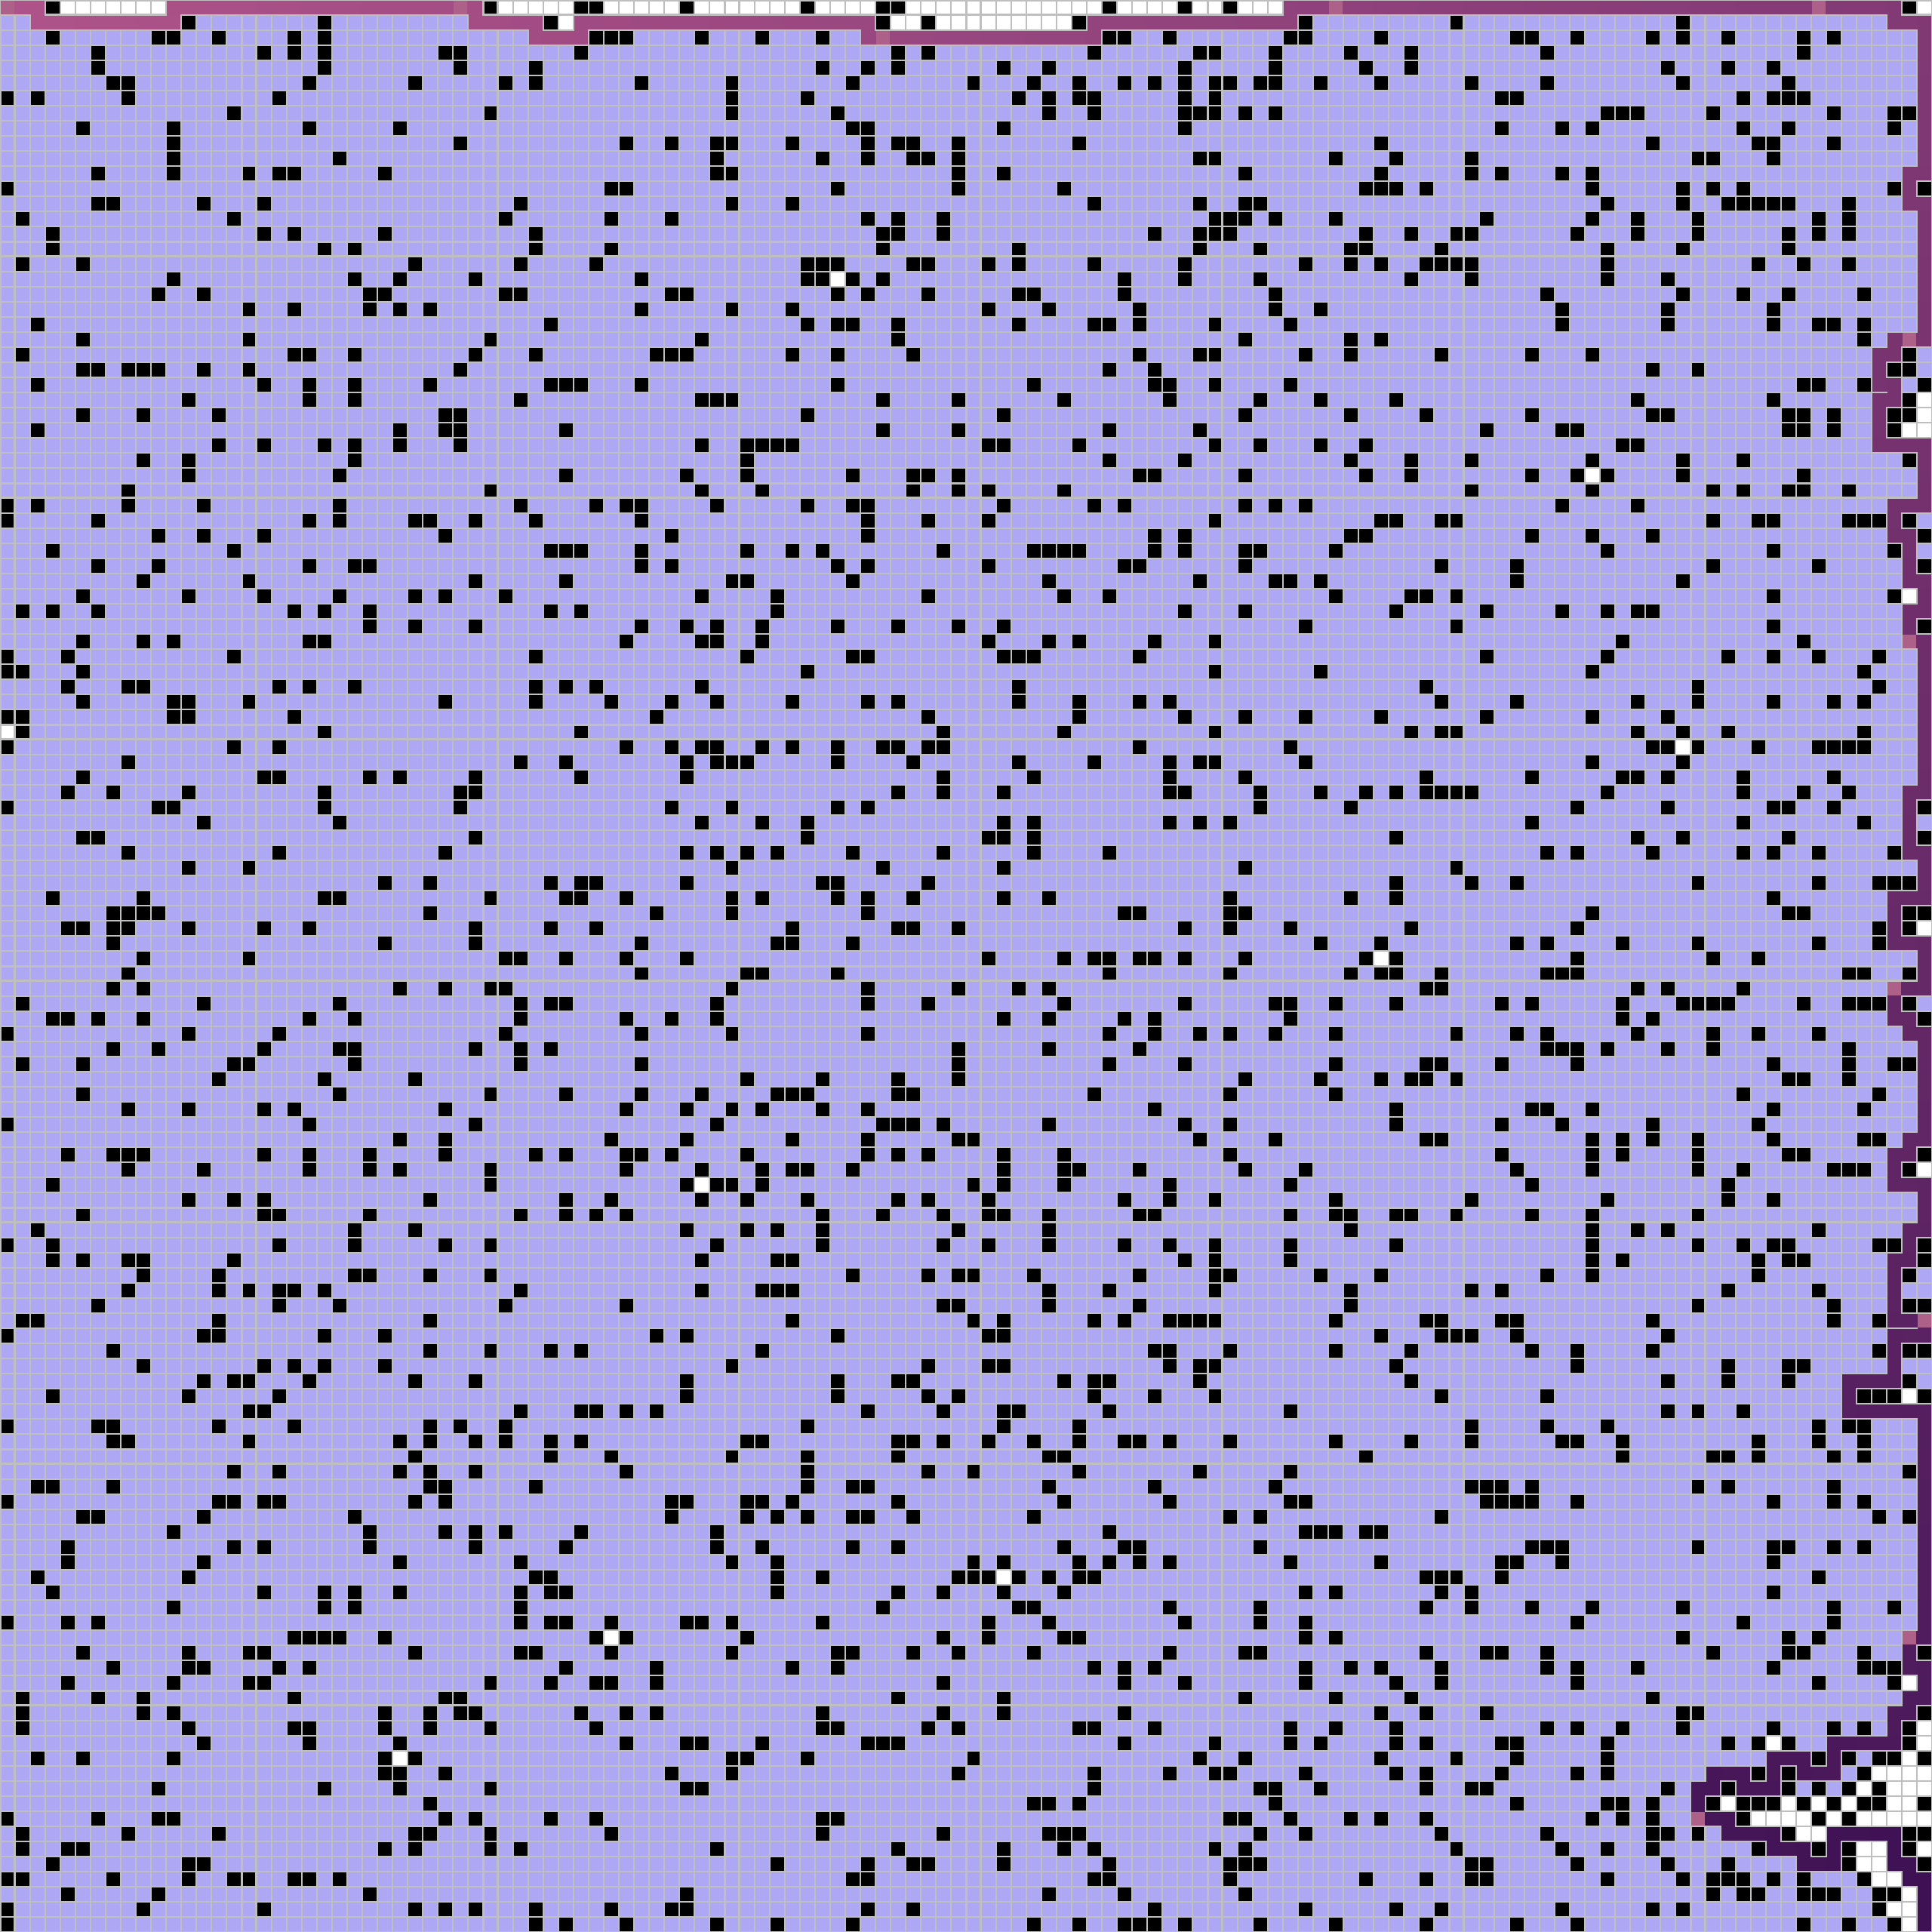
\includegraphics[width=\textwidth]{../pics/df/10031.png}
					\caption{\label{fig:df3} A maze that is hard for BFS in terms of space complexity, whose maximum fringe size is 10031. }
					\endminipage
					\endminipage 
				\end{figure}
				
				\textbf{Patterns or trends:} 
				\begin{itemize}
					\item {The same pattern as Question 10.b.ii, but there should be a clear path along the first row and upper half of the last column.}
				\end{itemize}
				
				\textbf{Reasons:} 
				\begin{itemize}
					\item {The time complexity of DFS related to the maximum depth it has searched.}
					\item {Hence, a "door sill" pattern can force DFS to search lower left part rather than immediately reach the Goal, which increased the maximum depth of DFS.}
					\item {A larger lower left part increases the depth, so the upper right part should be as small as possible.}
				\end{itemize}
				
				\textbf{"The hardest" maze:} 
				\begin{itemize}
					\item {The same maze as Question 10.b.ii.}
					\item {The maximum fringe size is theoretically $(size-1)^2-WallCost = 16113$, compared with 10032. Noticed distinctFringe actually do not promise all elements in the fringe are distinct because it takes too much time to search in a stack frequently. (Further information is available in description.md)}
					\item {Again, it is really difficult to cancel out those outside walls by random without destroying the pattern. Therefore, it has been a nearly "hardest" maze.}
				\end{itemize}
			\end{enumerate}
		
			\item {BFS} \\
			\label{BFS}
			The configuration of BFS is set to 'quickGoal' : True, 'checkFringe' : True, and all others are False. \\
			\begin{enumerate}
				\item {Length of solution path returned: See Figure \ref{fig:bp1}, Figure \ref{fig:bp2} and Figure \ref{fig:bp3}.} \\
				\begin{figure}
					\minipage{\textwidth}
					
					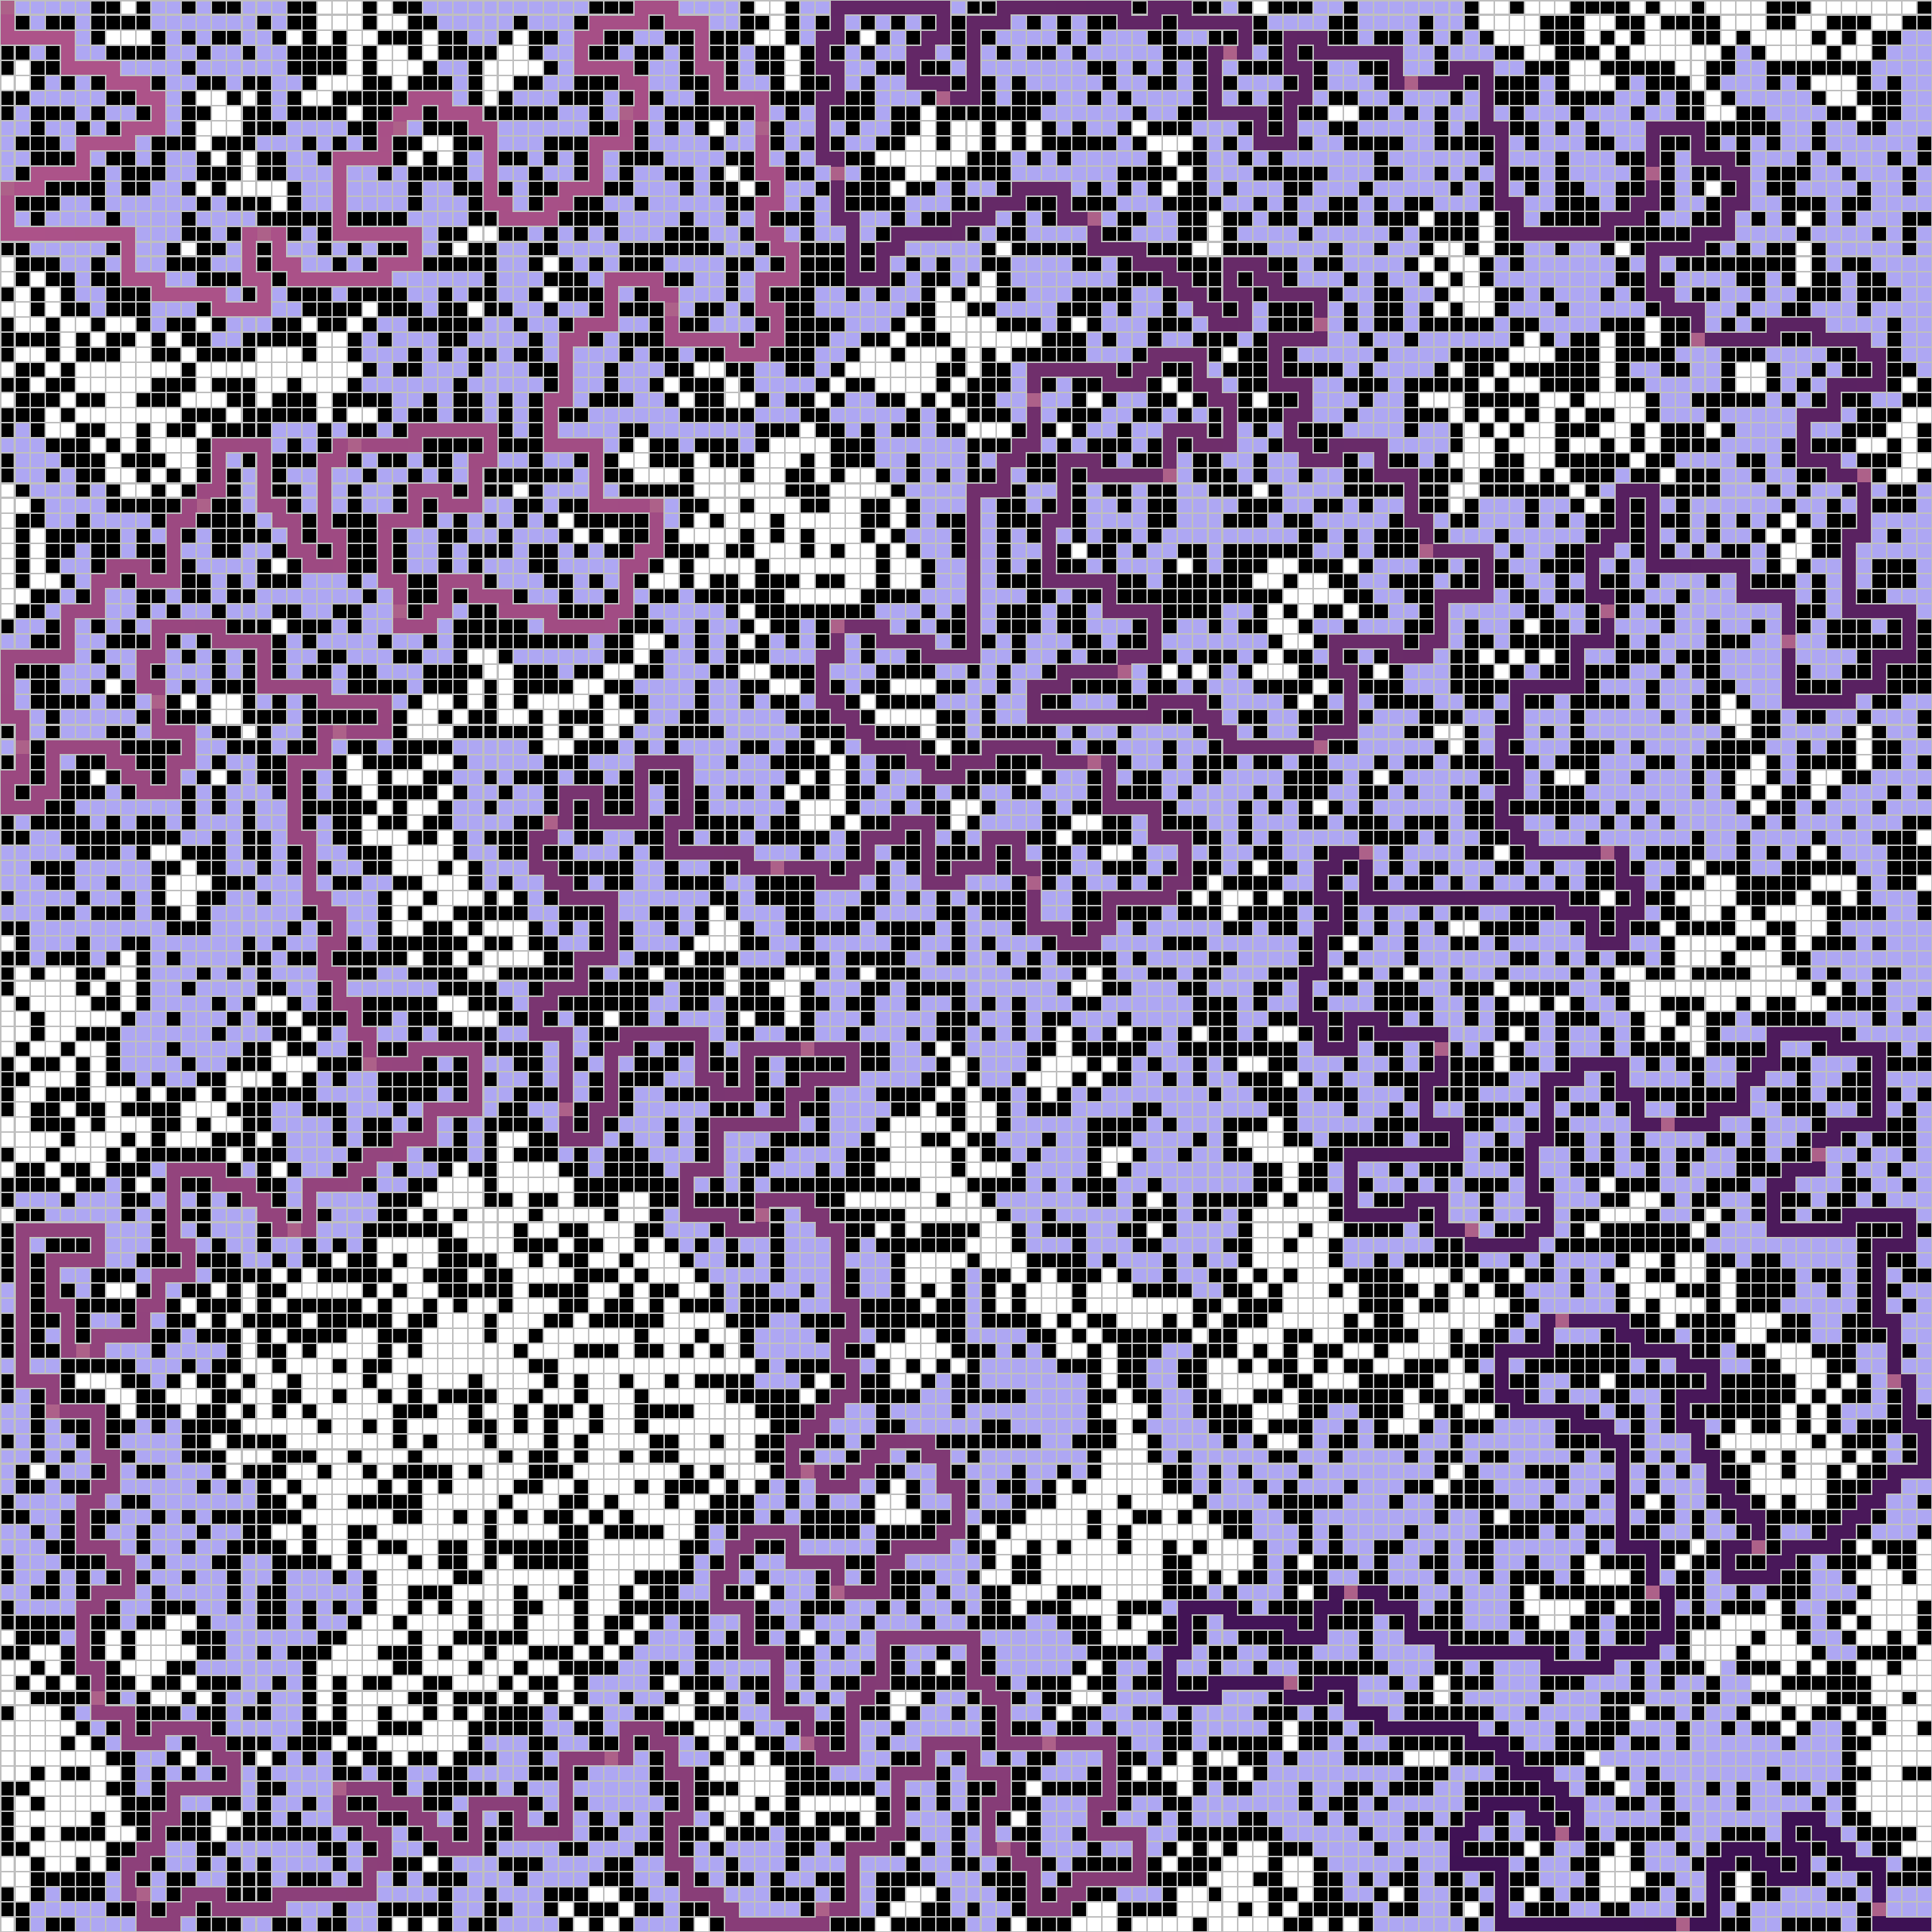
\includegraphics[width=\textwidth]{../pics/bp/2117.png}
					\caption{\label{fig:bp1}maze that is hard for BFS in terms of path length, which is 2117.}
					
					\minipage{0.49\textwidth}
					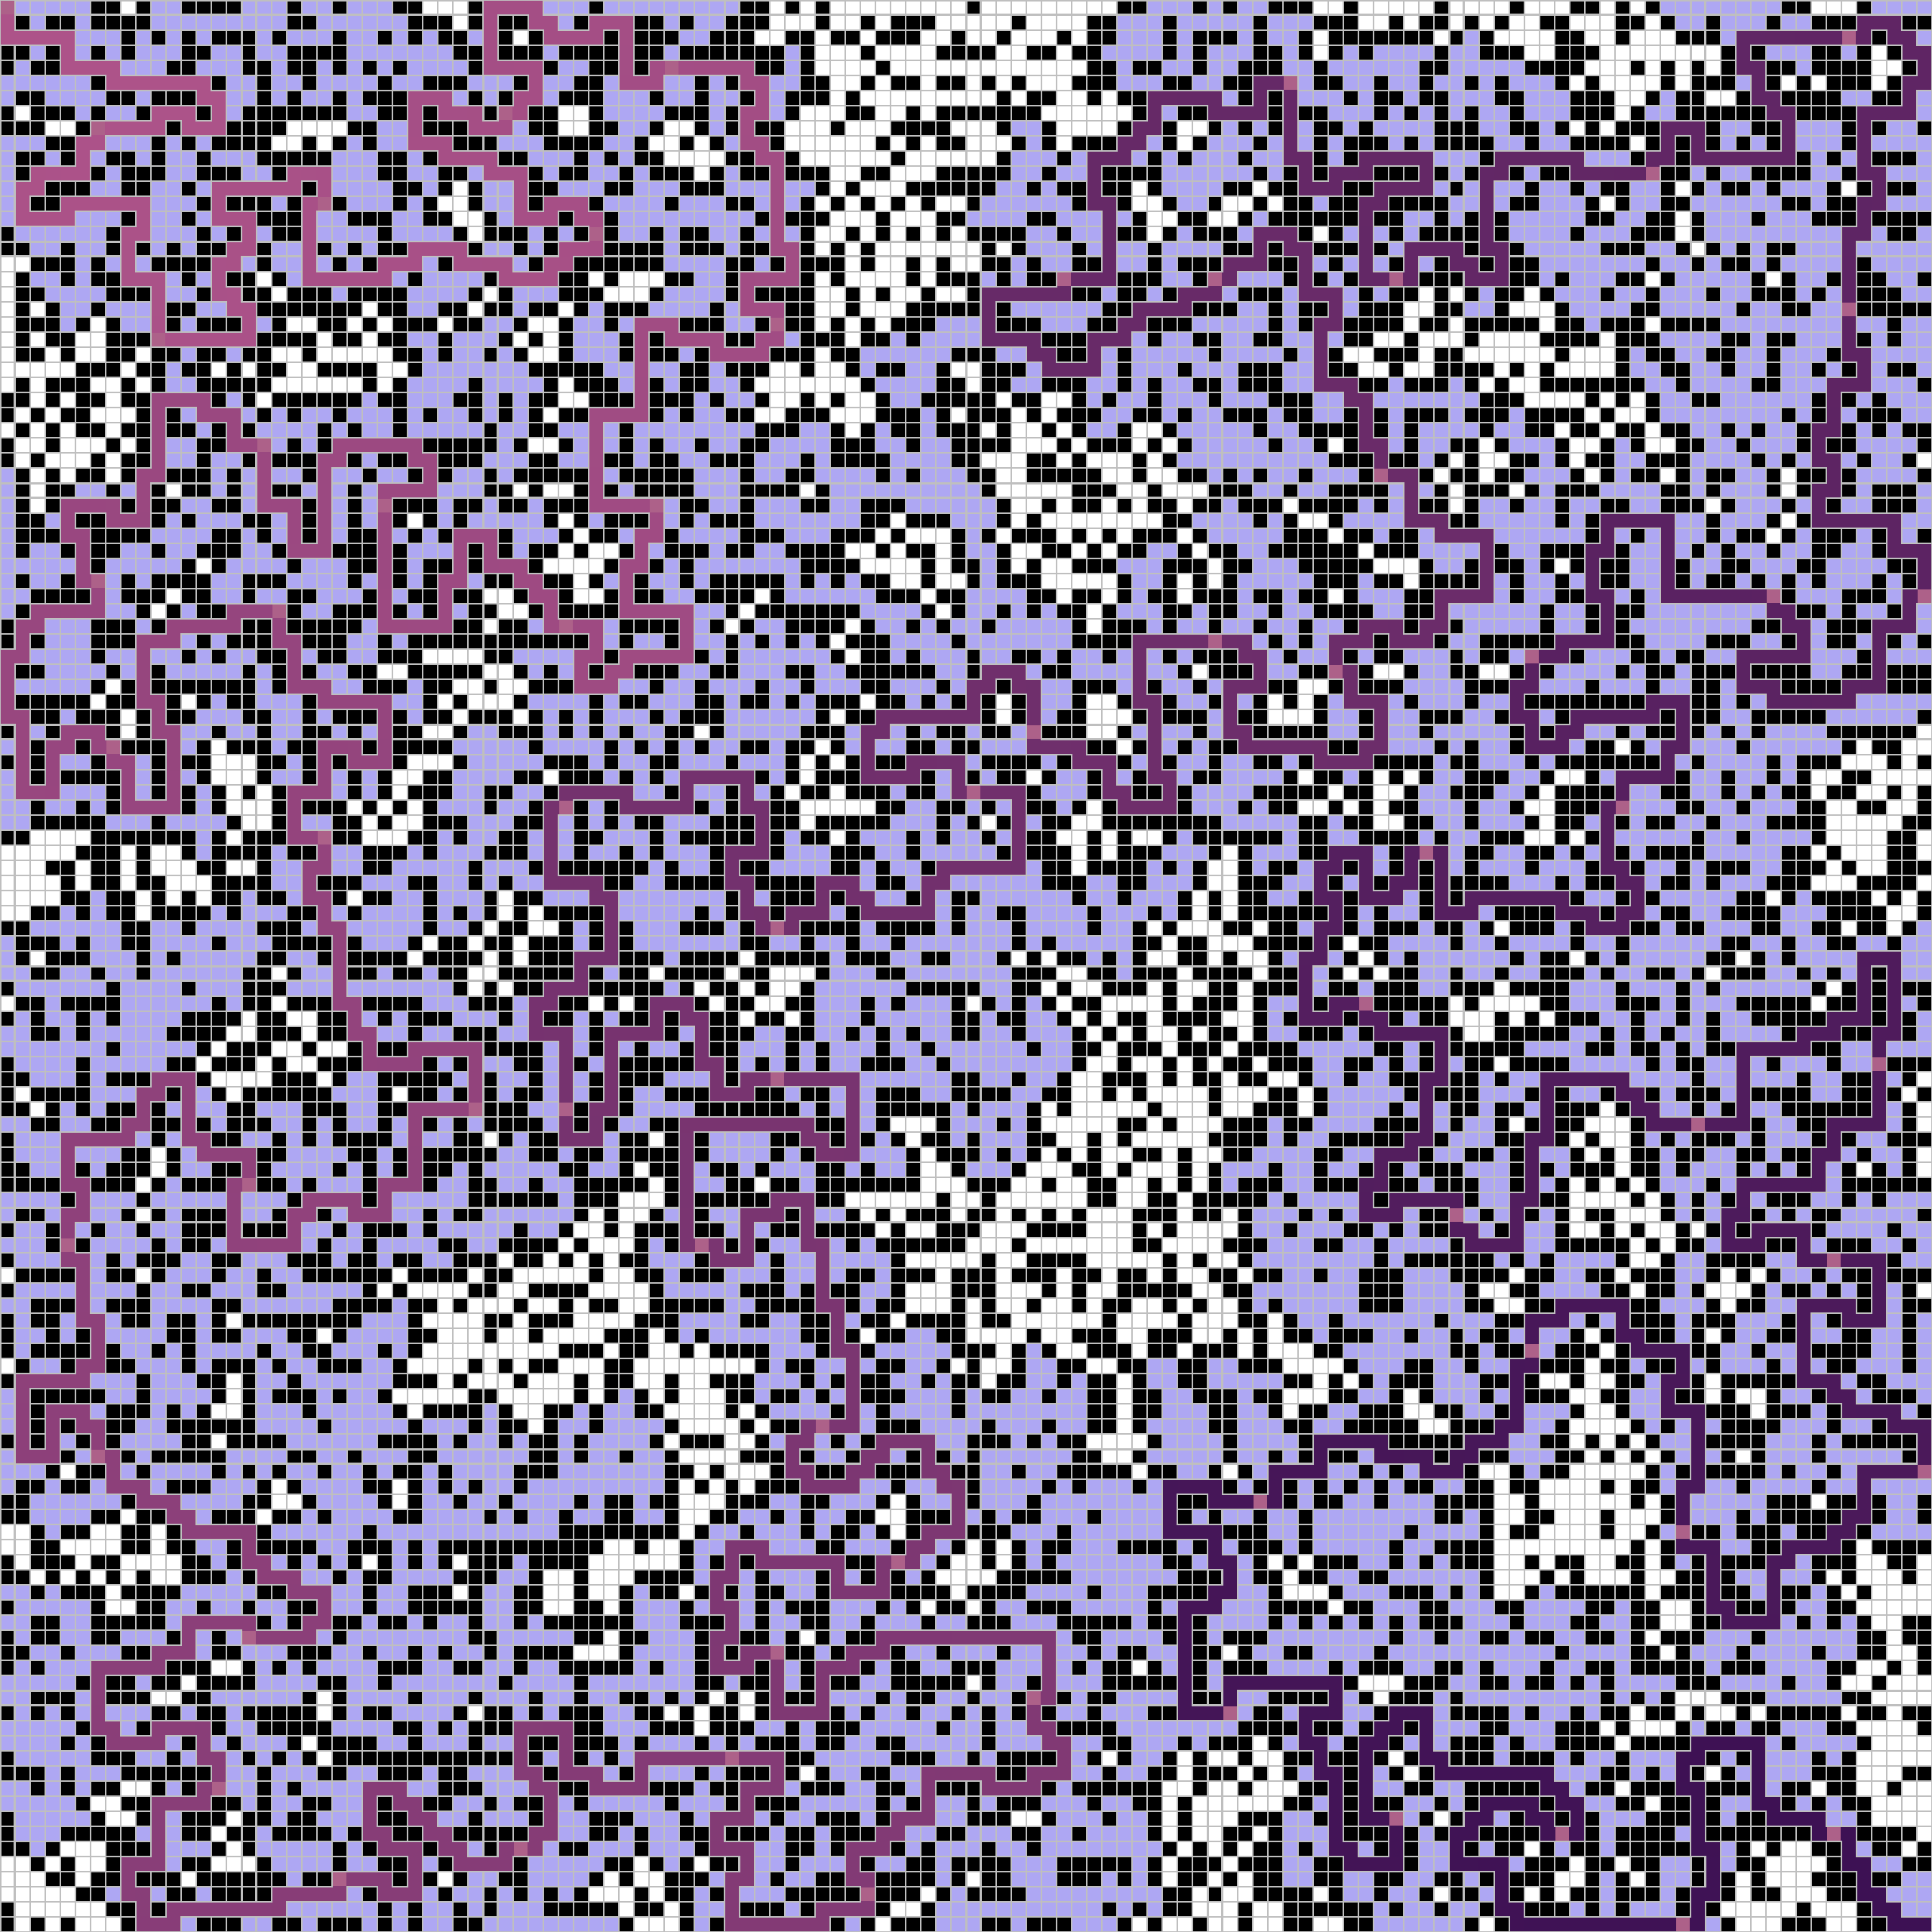
\includegraphics[width=\textwidth]{../pics/bp/2093.png}
					\caption{\label{fig:bp2}maze that is hard for BFS in terms of path length, which is 2093.}
					\endminipage\hfill
					\minipage{0.49\textwidth}
					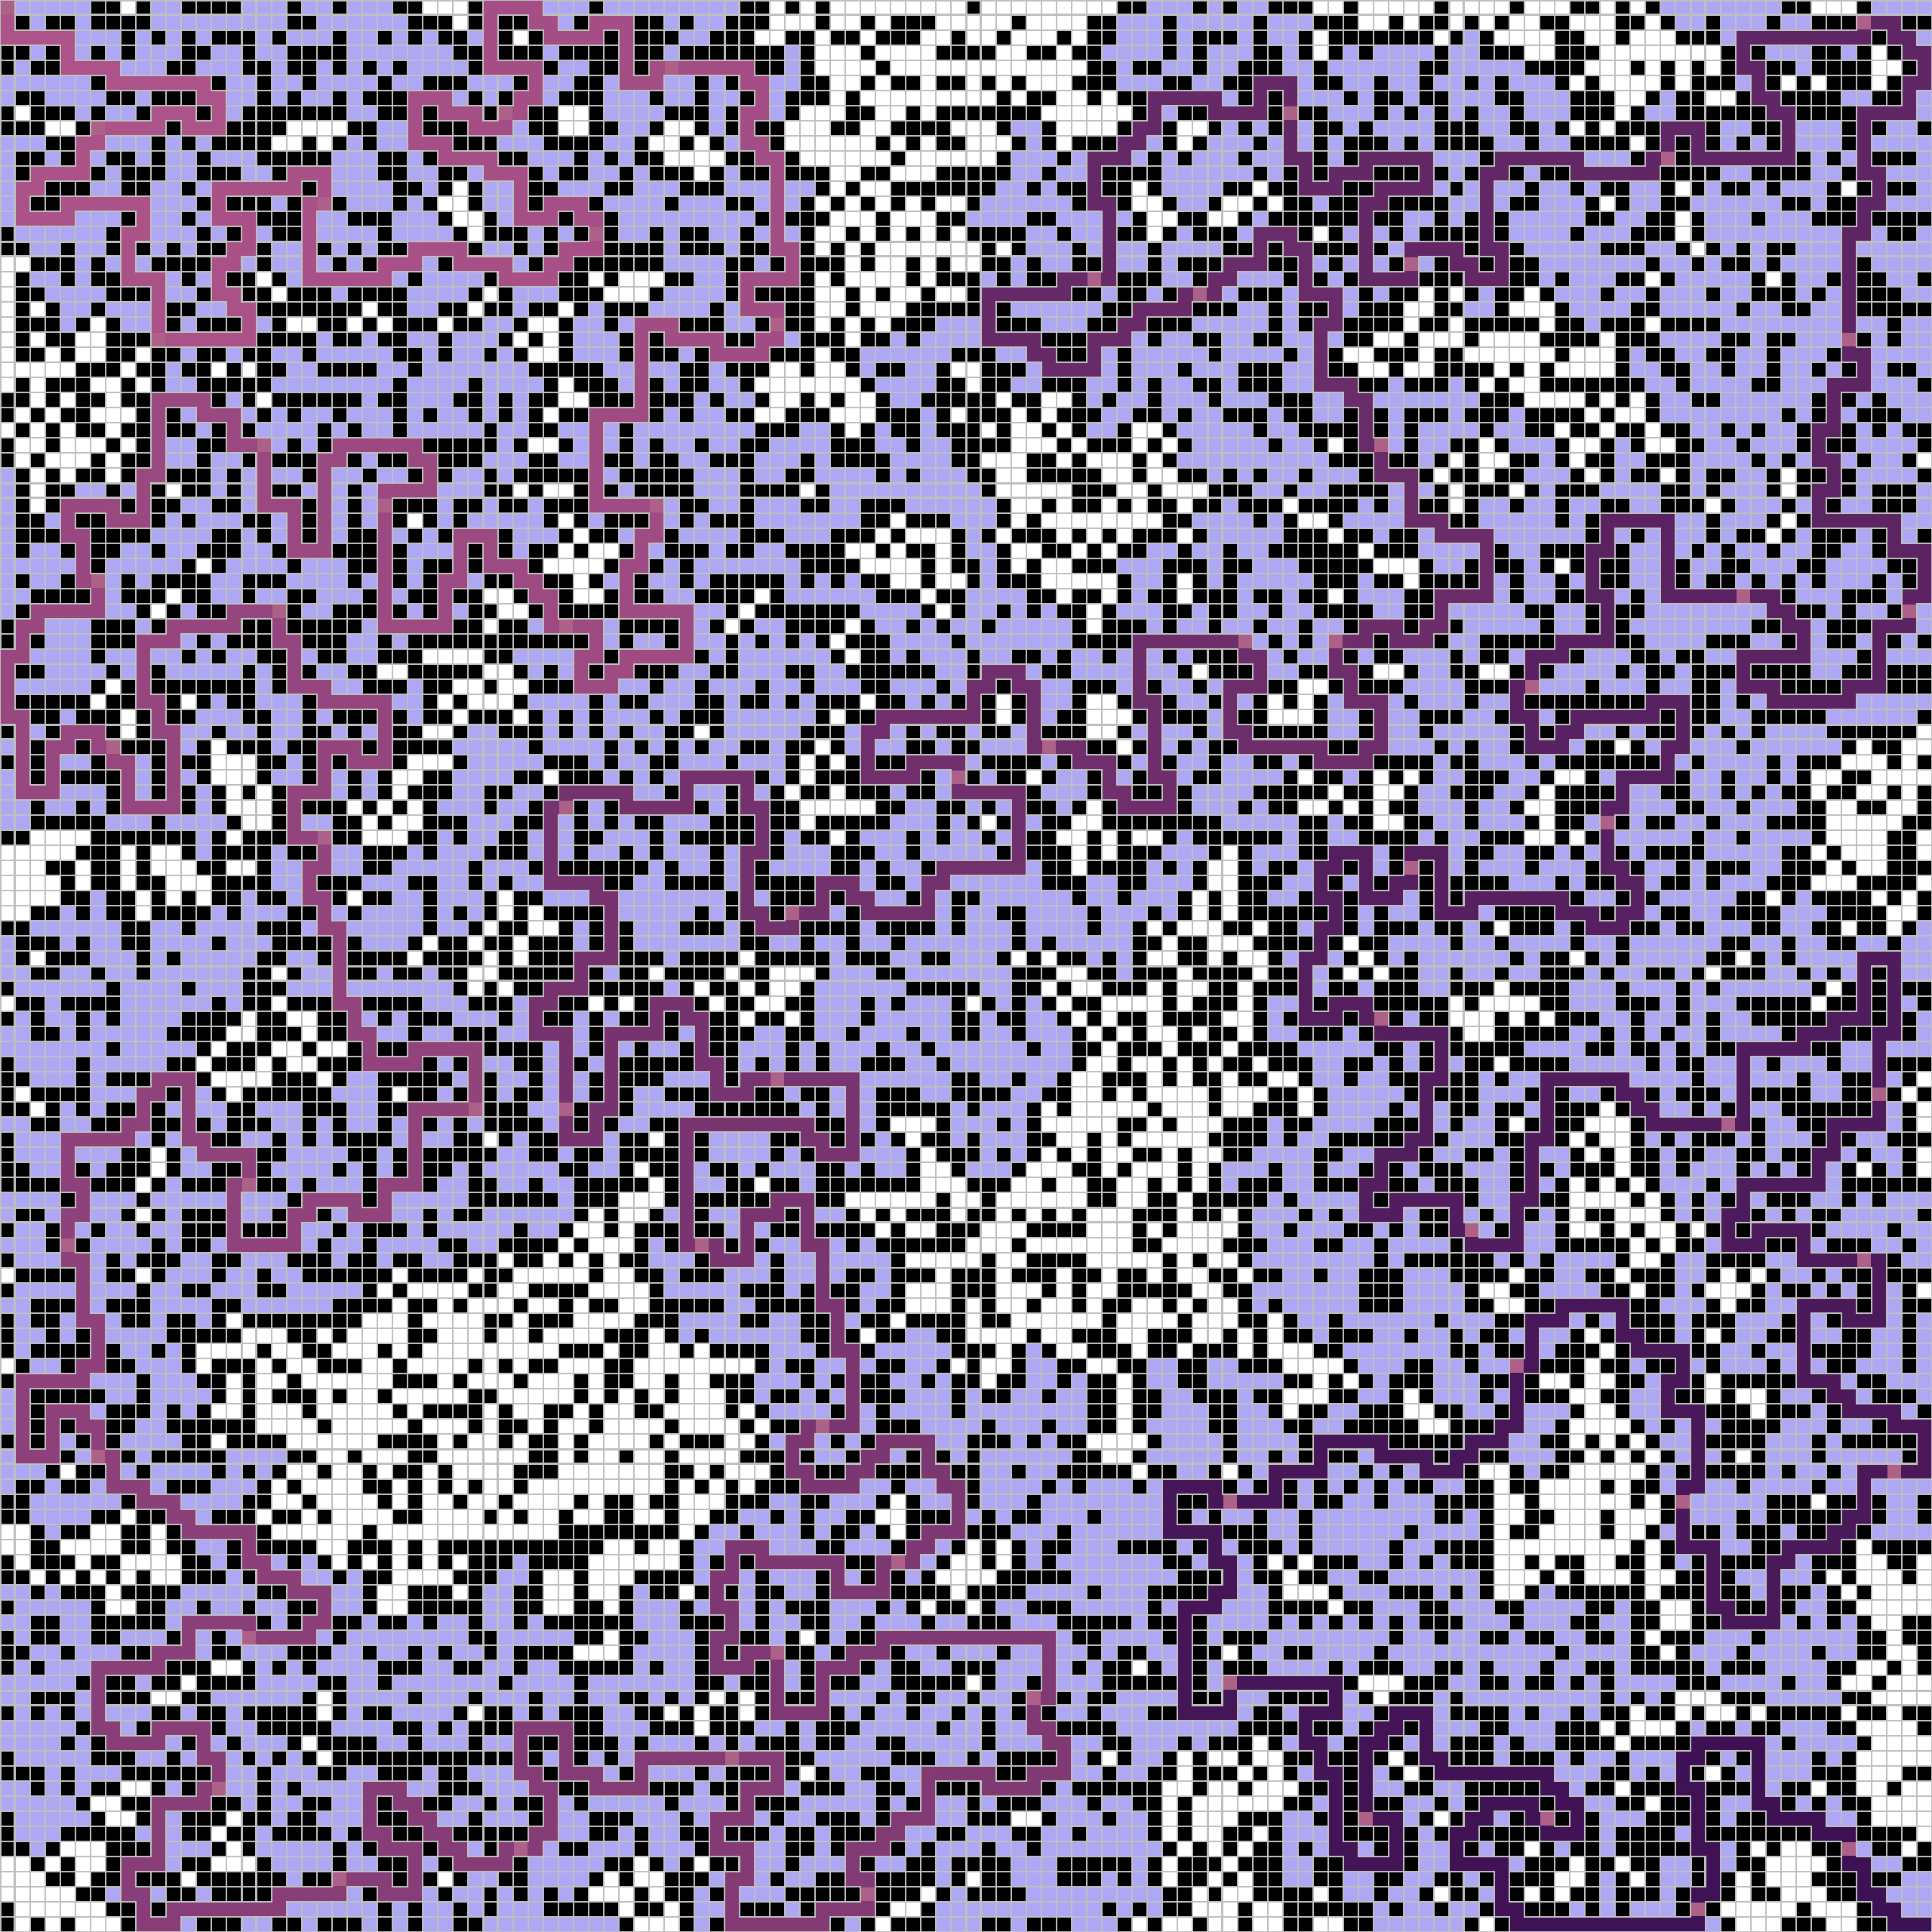
\includegraphics[width=\textwidth]{../pics/bp/2091.png}
					\caption{\label{fig:bp3}maze that is hard for BFS in terms of path length, which is 2091.}
					\endminipage
					\endminipage
					
				\end{figure}
				\textbf{Patterns or trends:} 
				\begin{itemize}
					\item {The path looks like a Hilbert curve, and as time goes, the path gets more and more sinuous.}
					\item {Walls are closely next to the path.}
				\end{itemize}
				
				\textbf{Reasons:} 
				\begin{itemize}
					\item {It is true that the path can also look like a “Gluttonous Snake”, which goes down to the bottom, walk right for 2 blocks, goes up to the top, walk right for 2 blocks, and repeat. However, it is hard to generate walls lined up just by random, so a Hilbert-curve-like maze is more probable.}
					\item {Hilbert curve can theoretically reach every point of a plane, i.e., its length can be the maximum.}
				\end{itemize}
				
				\textbf{"The hardest" maze:} 
				\begin{itemize}
					\item {There are 2 kinds of the "hardest" maze: “Gluttonous-Snake-like” mazes and Hilbert-curve-like mazes. Both of them can let the path length reached $\frac{size * size}{2} = 8192$, where the 2 is the cost of building walls to limit the path.}
					\item {Compared with 8192, 2117 is not "hard" enough. It is also presented in Fig 2.10.5 that there are still many blocks totally unused. However, due to the time limitation, we cannot run the iterations more times. Yet, 2117 compared with 500 in Question 4(Notice that the size of mazes in Question 4 is 200, which is larger than 128.) can be regarded as a "harder" maze.}
					\item {Also, it is interesting to take the maximum fringe size into account. The ideal "hardest" maze's fringe size can be always 1 because there is only one path whose width is also 1 to reach the Goal. Hence, the maximum fringe size can also measure how close we get to the "hardest" maze. But notice that not all mazes whose max fringe size is 1 are "hardest" maze, due to the fact that the path can directly go diagonally. Table \ref{Table 2} shows the fringe size and path length of top 5 "harder" mazes we have generated.}
					\begin{center}
						\label{Table 2}
						\begin{tabular}{|c|c|c|}
							\hline
							Block & Path & Fringe \\
							\hline
							7013 & 2117 & 14 \\
							\hline
							7467 & 2093 & 18 \\
							\hline
							7293 & 2091 & 18 \\
							\hline
							7382 & 2069 & 27 \\
							\hline
							7433 & 2069 & 26 \\
							\hline
						\end{tabular}
						\captionof{table}{}
					\end{center}
				\end{itemize}
				
				\item {Total number of nodes expanded: See Figure \ref{fig:bb1}, Figure \ref{fig:bb2} and Figure \ref{fig:bb3}.} \\
				\begin{figure}
					\minipage{\textwidth}
					
					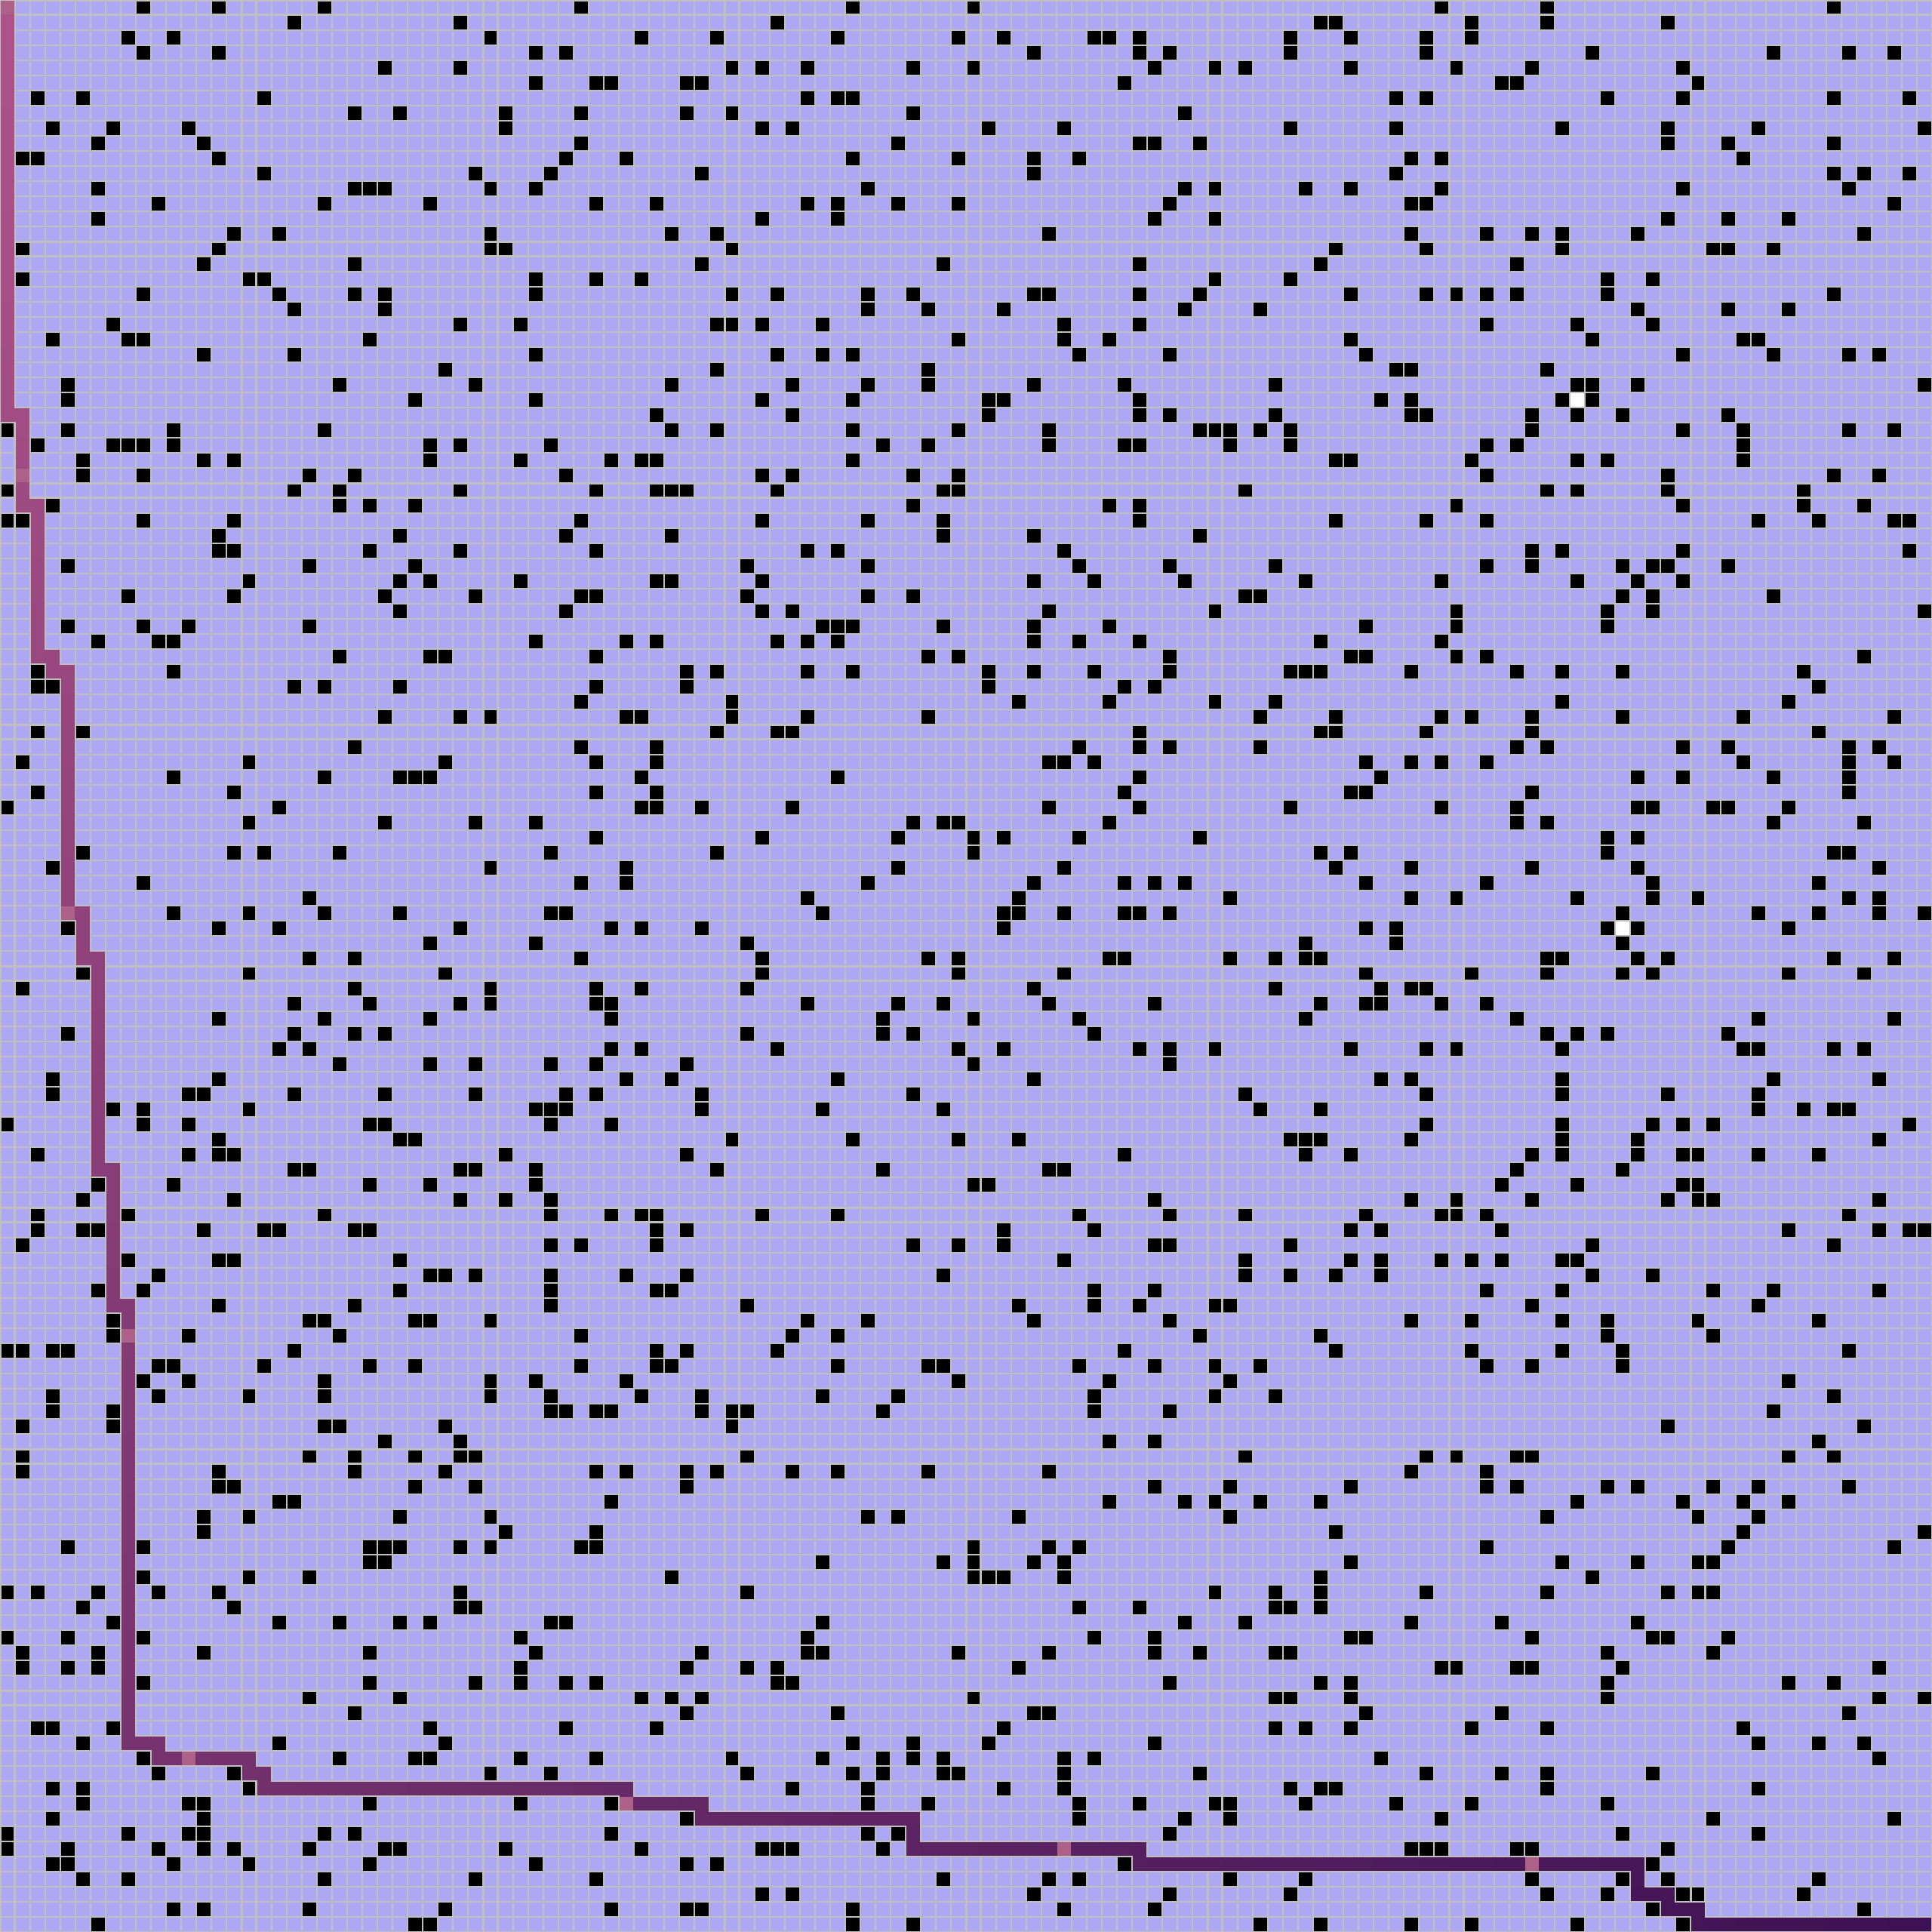
\includegraphics[width=\textwidth]{../pics/bb/14776.png}
					\caption{\label{fig:bb1}A maze that is hard for BFS in terms of time complexity, which has opend 14776 blocks.}
					
					\minipage{0.49\textwidth}
					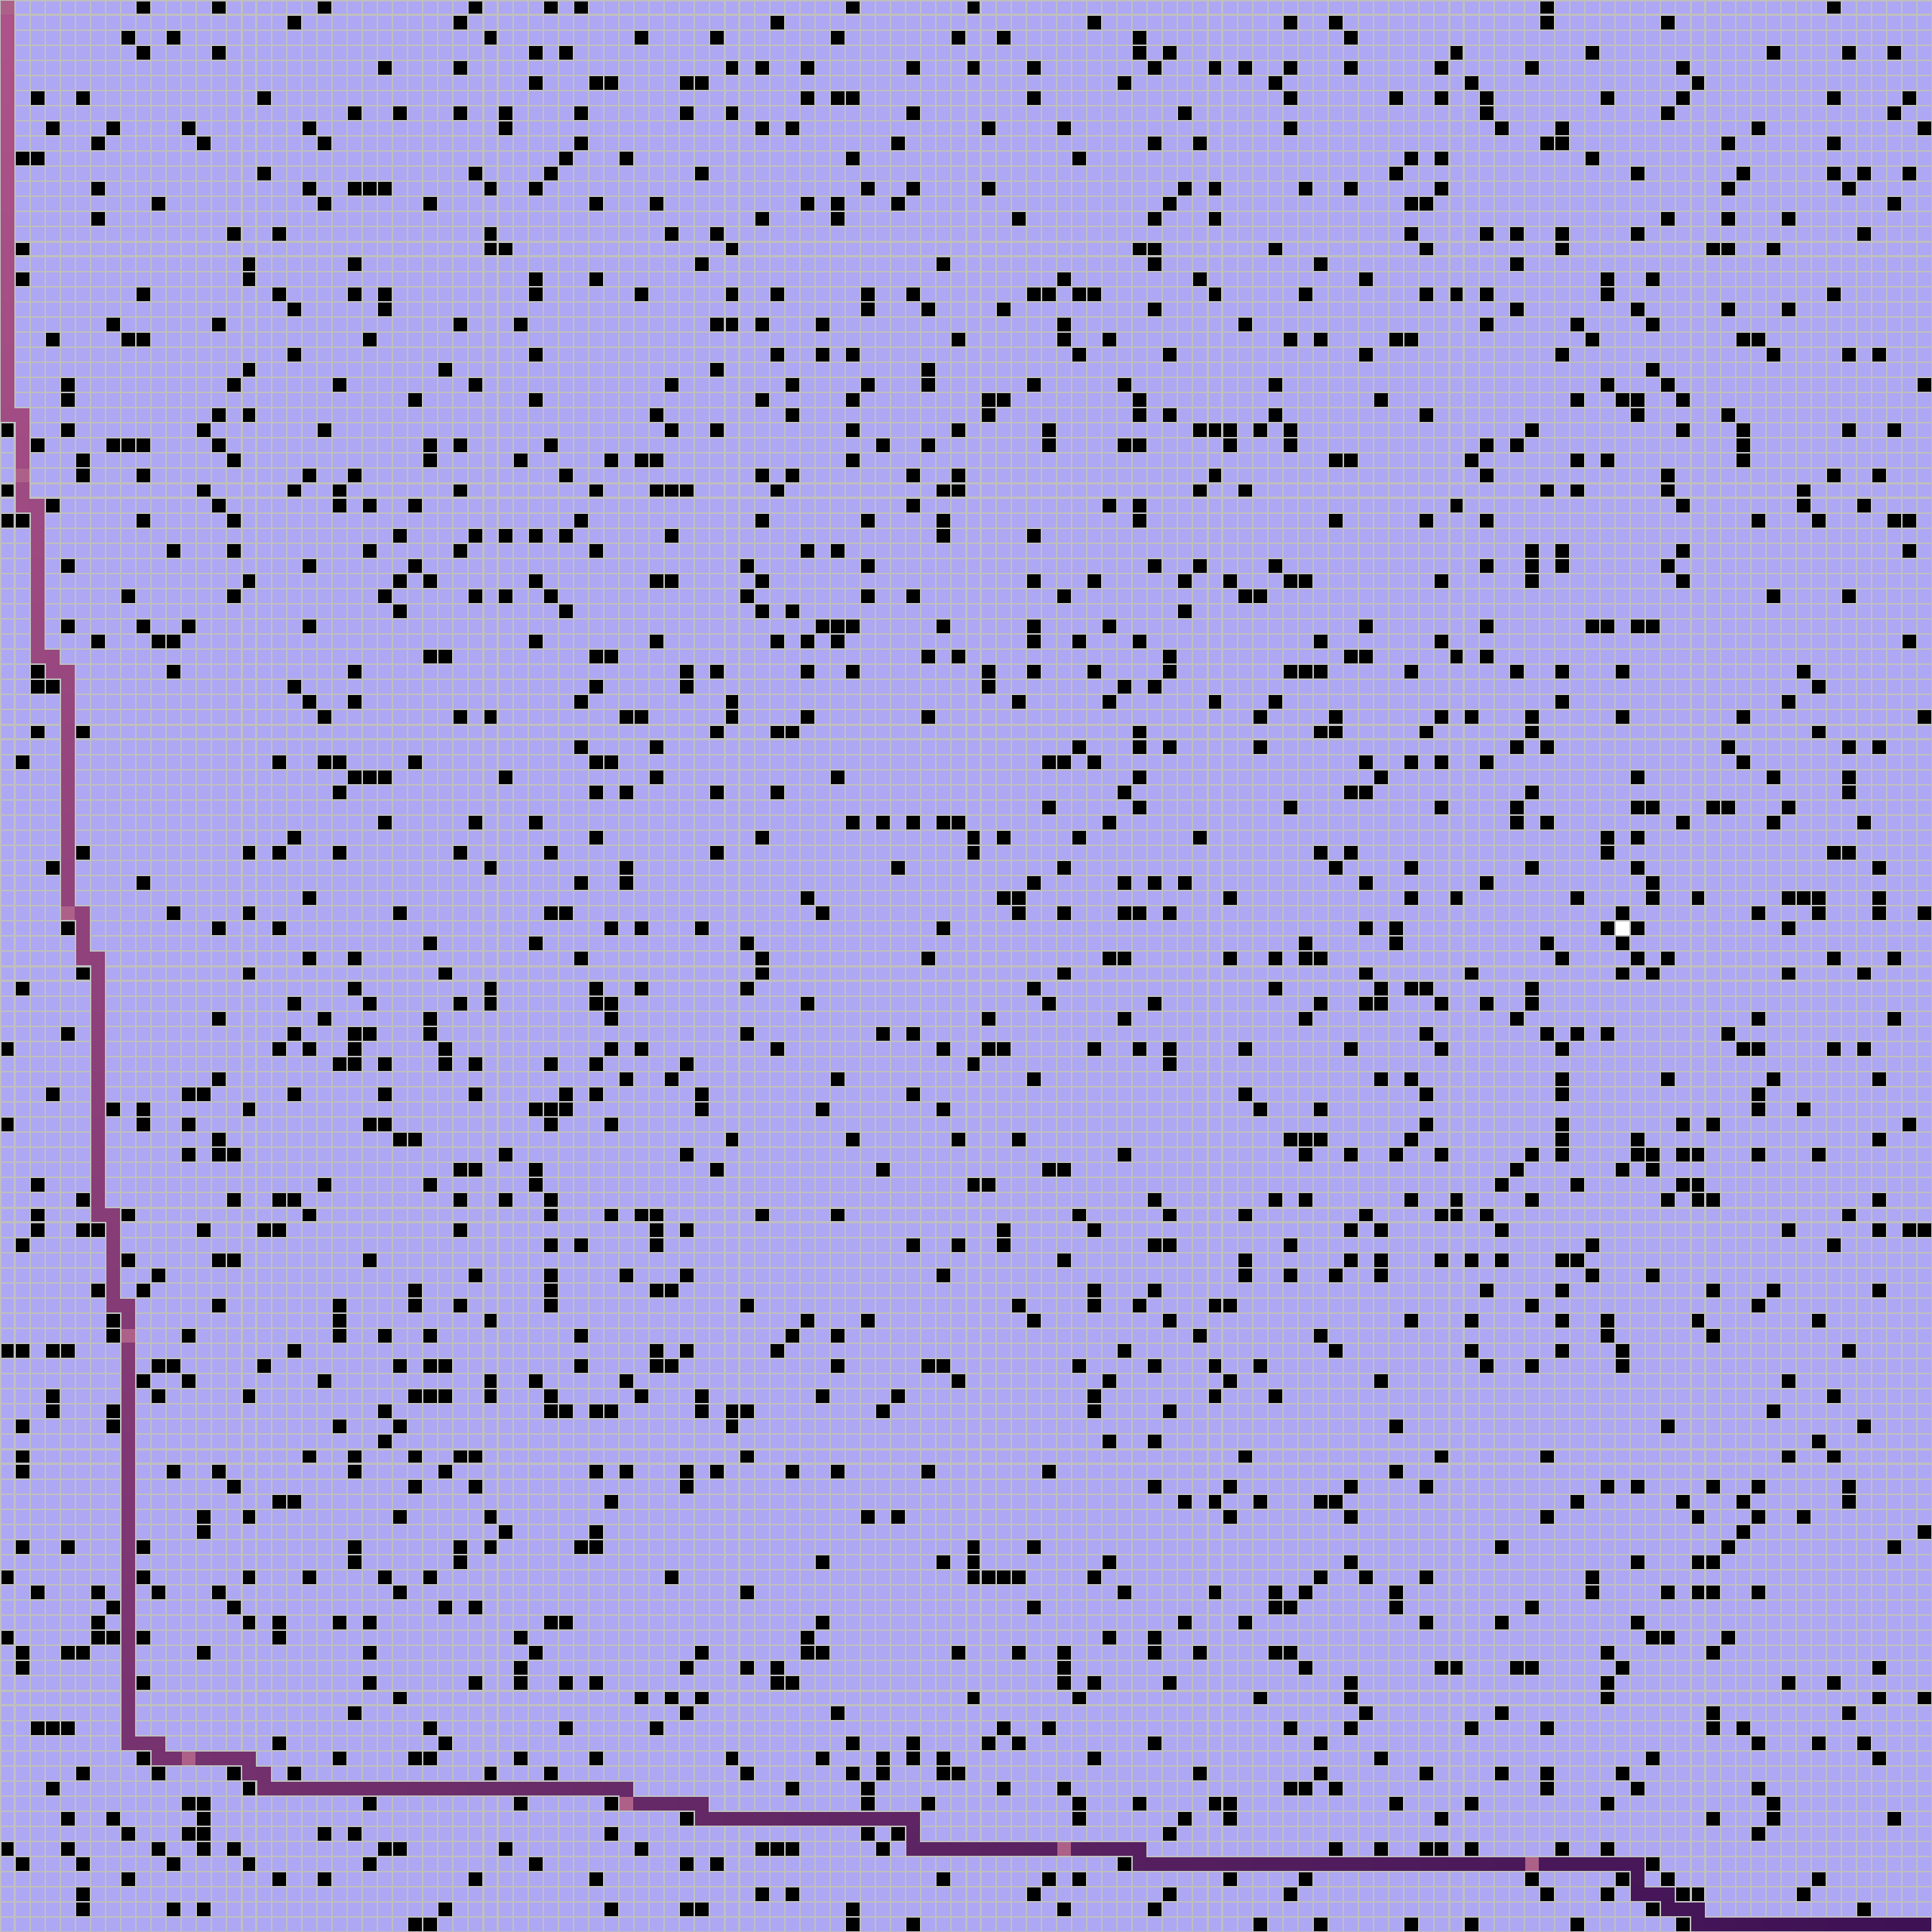
\includegraphics[width=\textwidth]{../pics/bb/14772_2.png}
					\caption{\label{fig:bb2}A maze that is hard for BFS in terms of time complexity, which has opend 14772 blocks.}
					\endminipage\hfill
					\minipage{0.49\textwidth}
					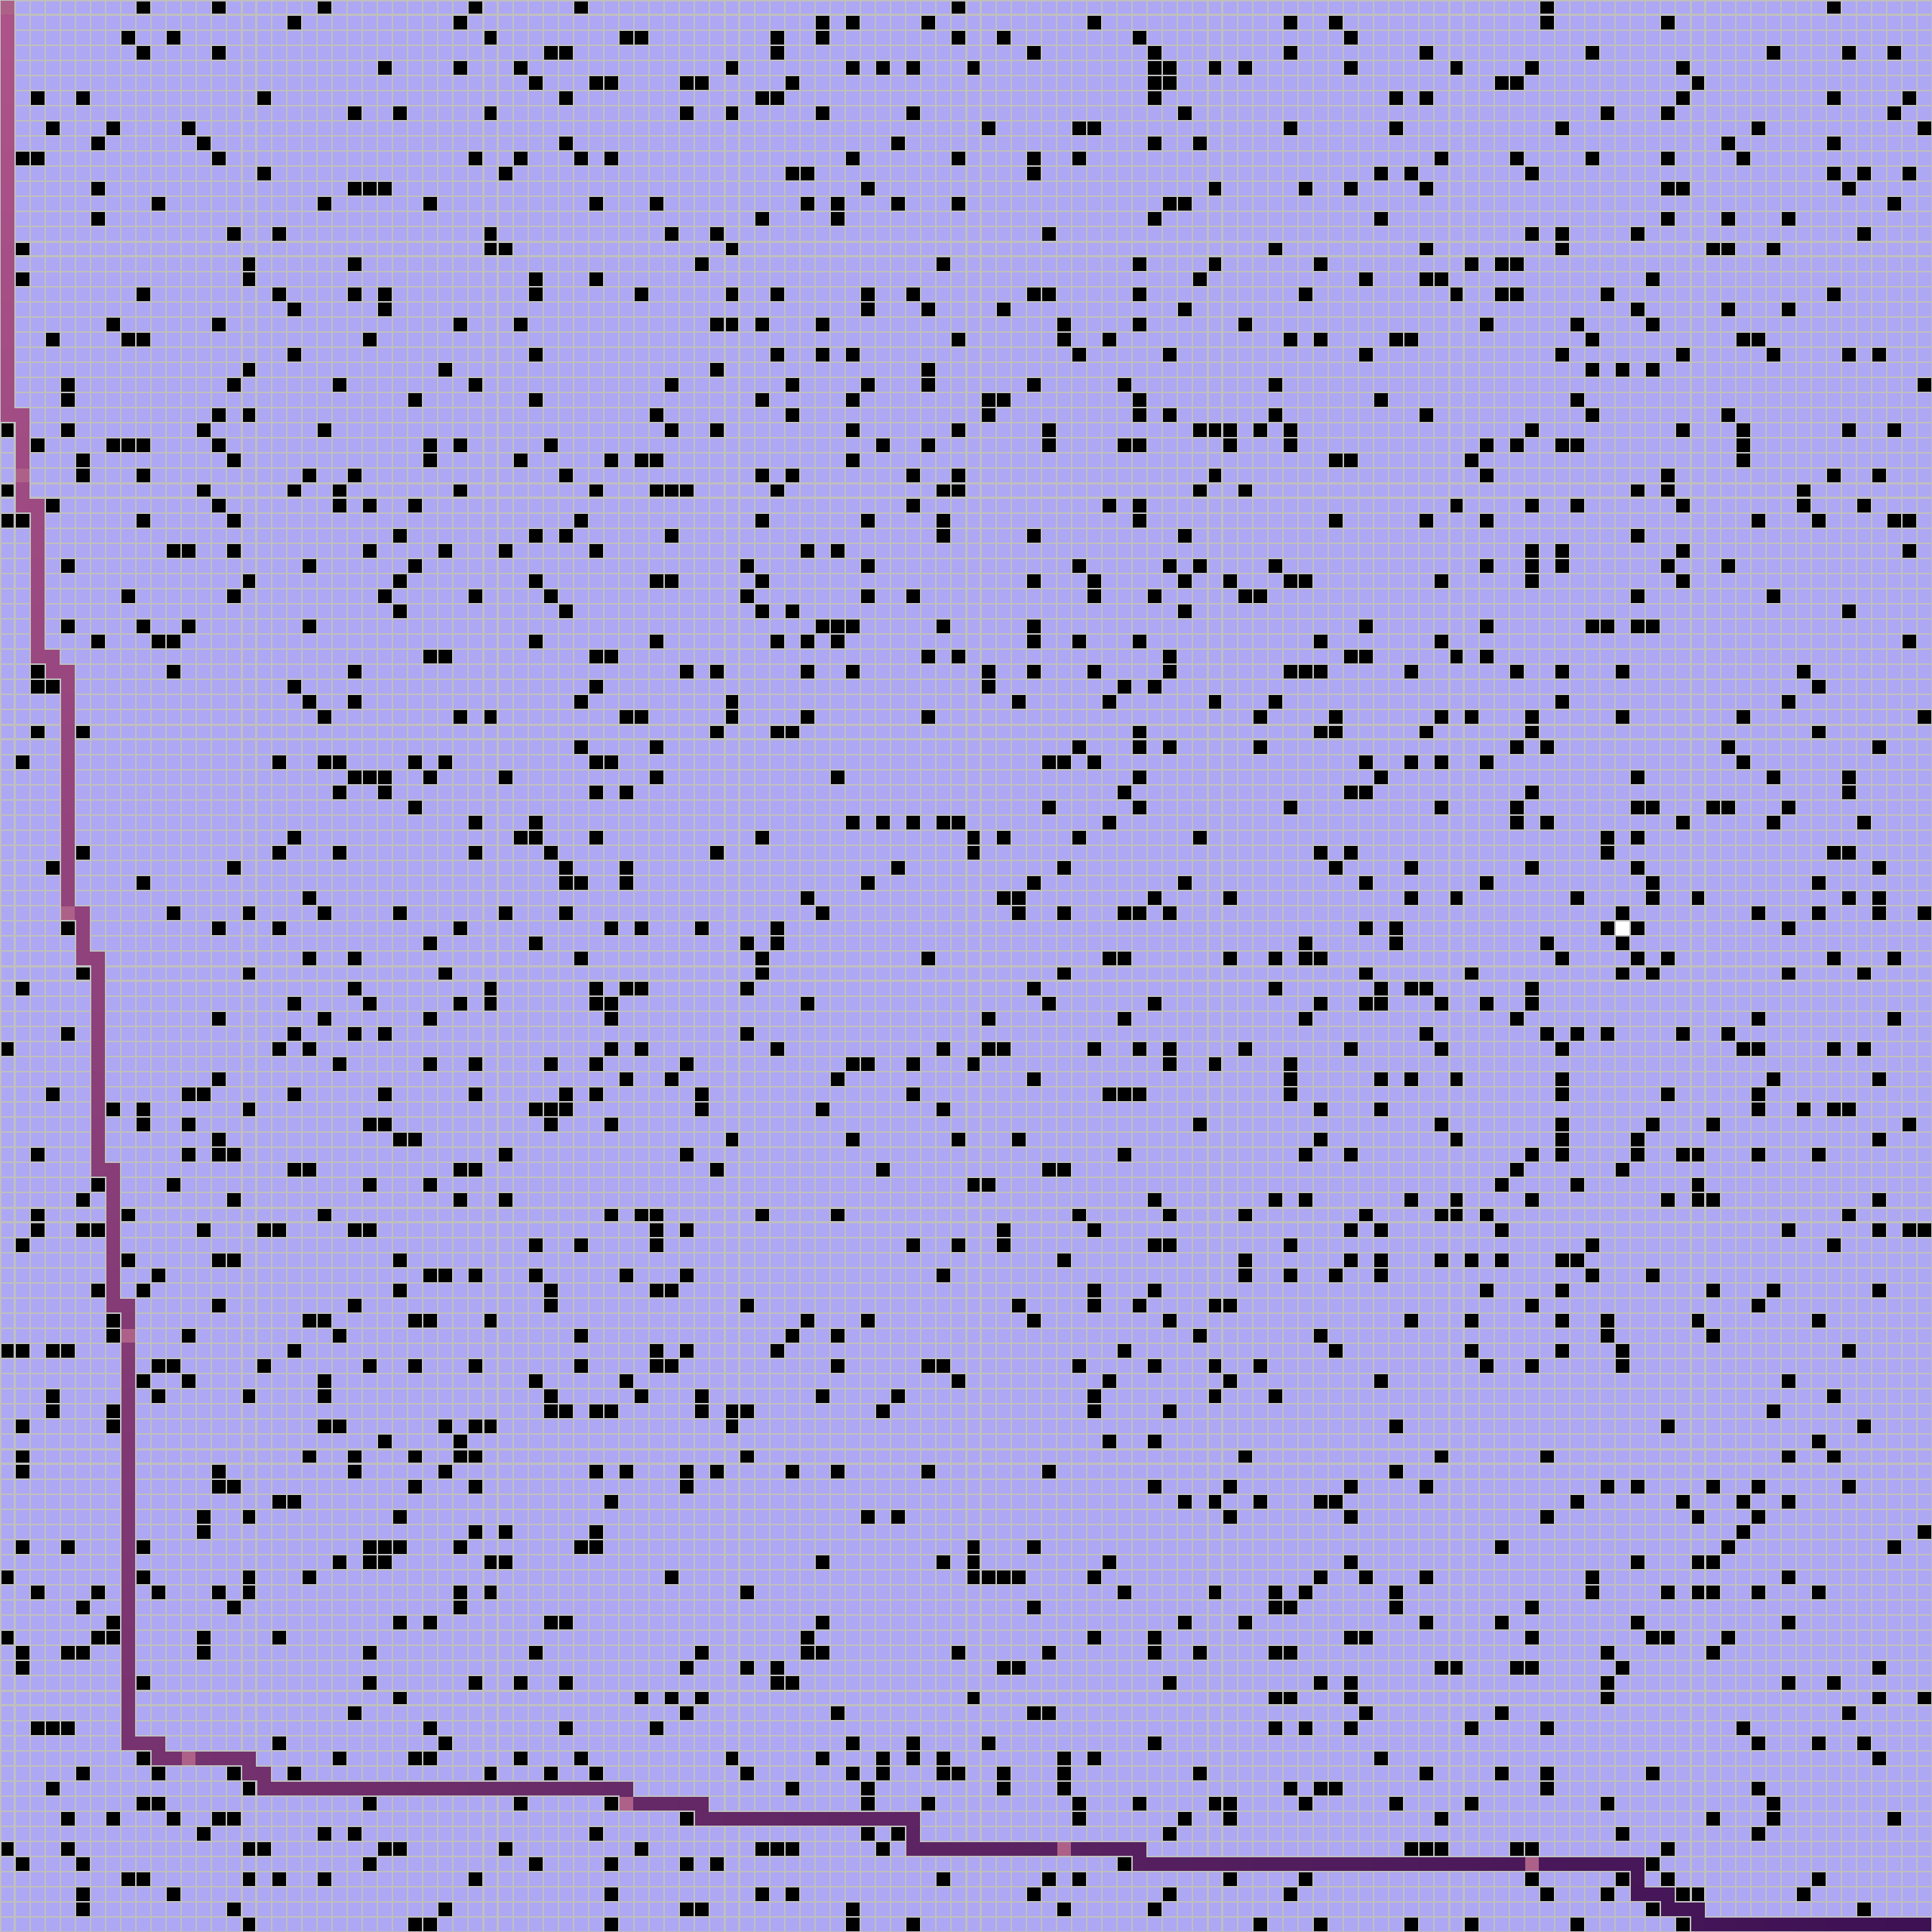
\includegraphics[width=\textwidth]{../pics/bb/14772.png}
					\caption{\label{fig:bb3} A maze that is hard for BFS in terms of time complexity, which has opend 14772 blocks.}
					\endminipage
					\endminipage 
				\end{figure}
				
				\textbf{Patterns or trends:} 
				\begin{itemize}
					\item {A nearly "empty"(no walls) maze is usually hard for BFS in terms of time complexity.}
				\end{itemize}
				
				\textbf{Reasons:} 
				\begin{itemize}
					\item {BFS will open shallower blocks first, and then move to deeper blocks.}
					\item {Usually, the Goal is the deepest block if the Start is located at 2 ends of a diagonal.}
					\item {In this case, BFS will open all the accessible blocks before reaching the Goal. The number of blocks opened is exactly the number of all accessible blocks of this maze.}
					\item {To make it harder is to make more blocks accessible. Namely, to delete more walls.}
				\end{itemize}
				
				\textbf{"The hardest" maze:} 
				\begin{itemize}
					\item {A totally "empty" maze whose number of blocks opened is exactly $size \times size = 16384$.}
					\item {The best score we have got is 14776, compared with at most 16384. However, it is really difficult to cancel out those walls by random. Therefore, it has been a nearly "hardest" maze.}
				\end{itemize}
				
				\item {Maximum size of fringe during runtime: See Figure \ref{fig:df1}, Figure \ref{fig:df2} and Figure \ref{fig:df3}.} \\
				\begin{figure}
					\minipage{\textwidth}
					
					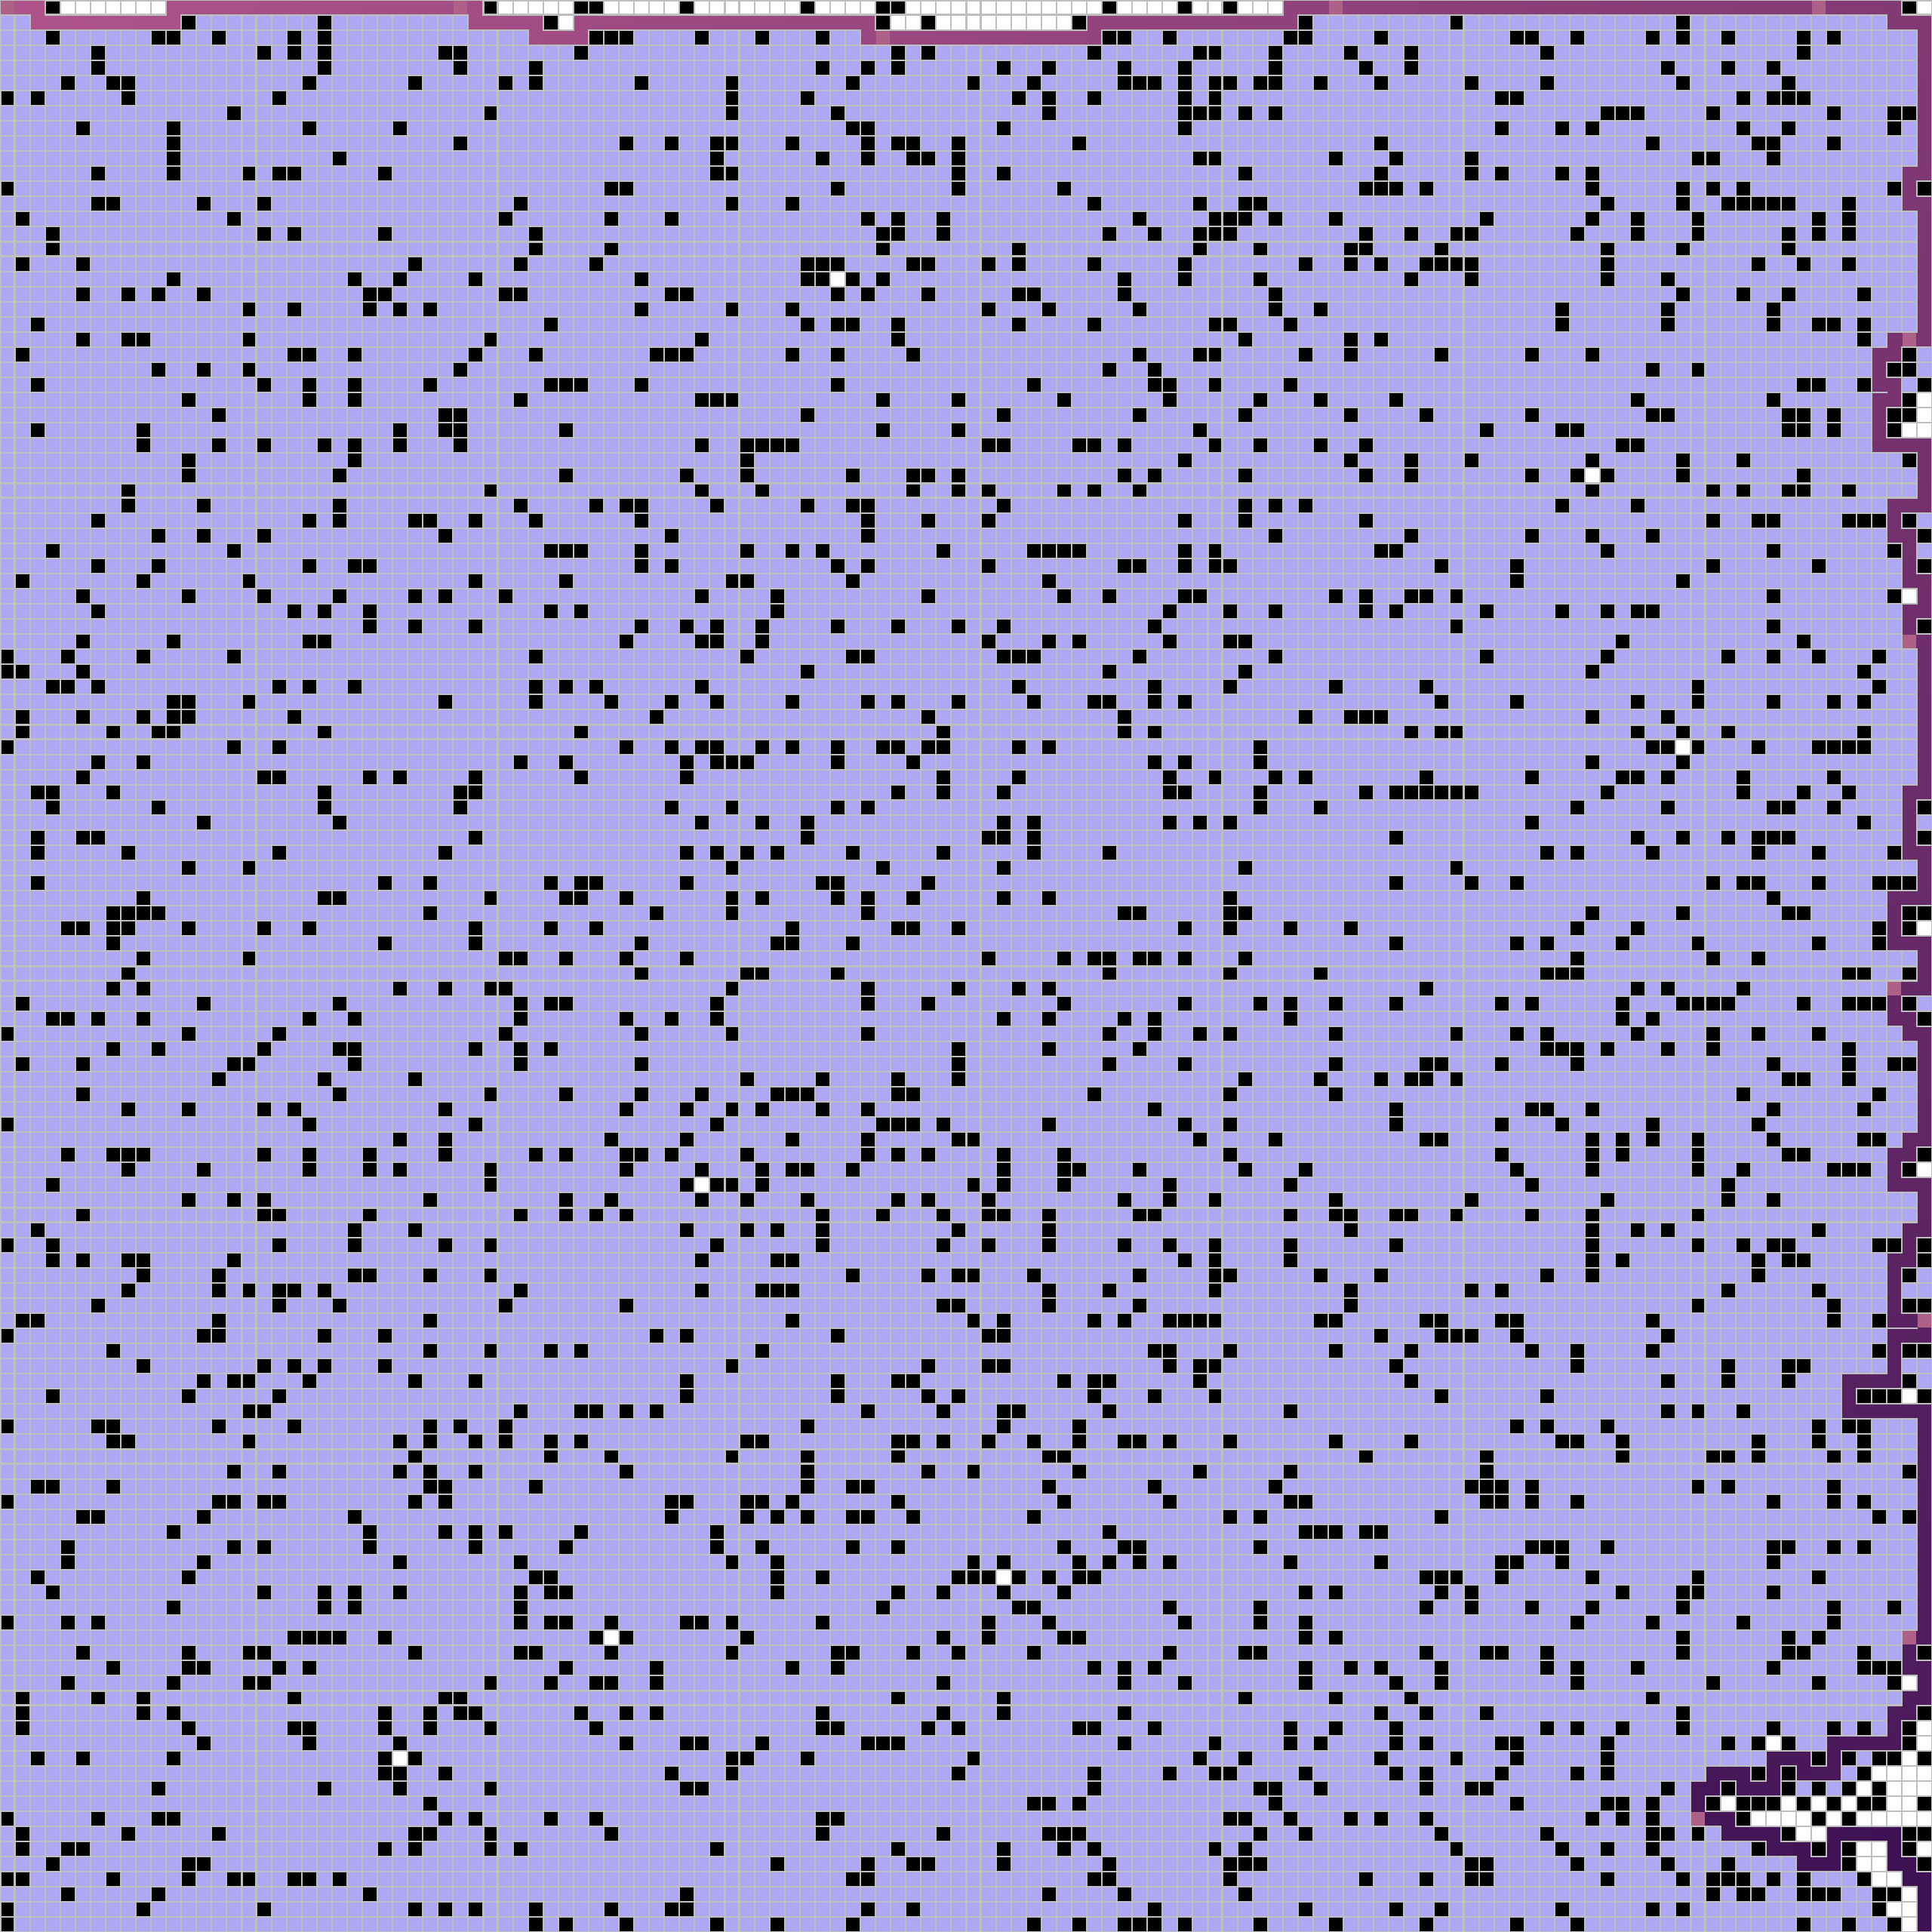
\includegraphics[width=\textwidth]{../pics/df/10032_2.png}
					\caption{\label{fig:df1}A maze that is hard for BFS in terms of space complexity, whose maximum fringe size is 10032. }
					
					\minipage{0.49\textwidth}
					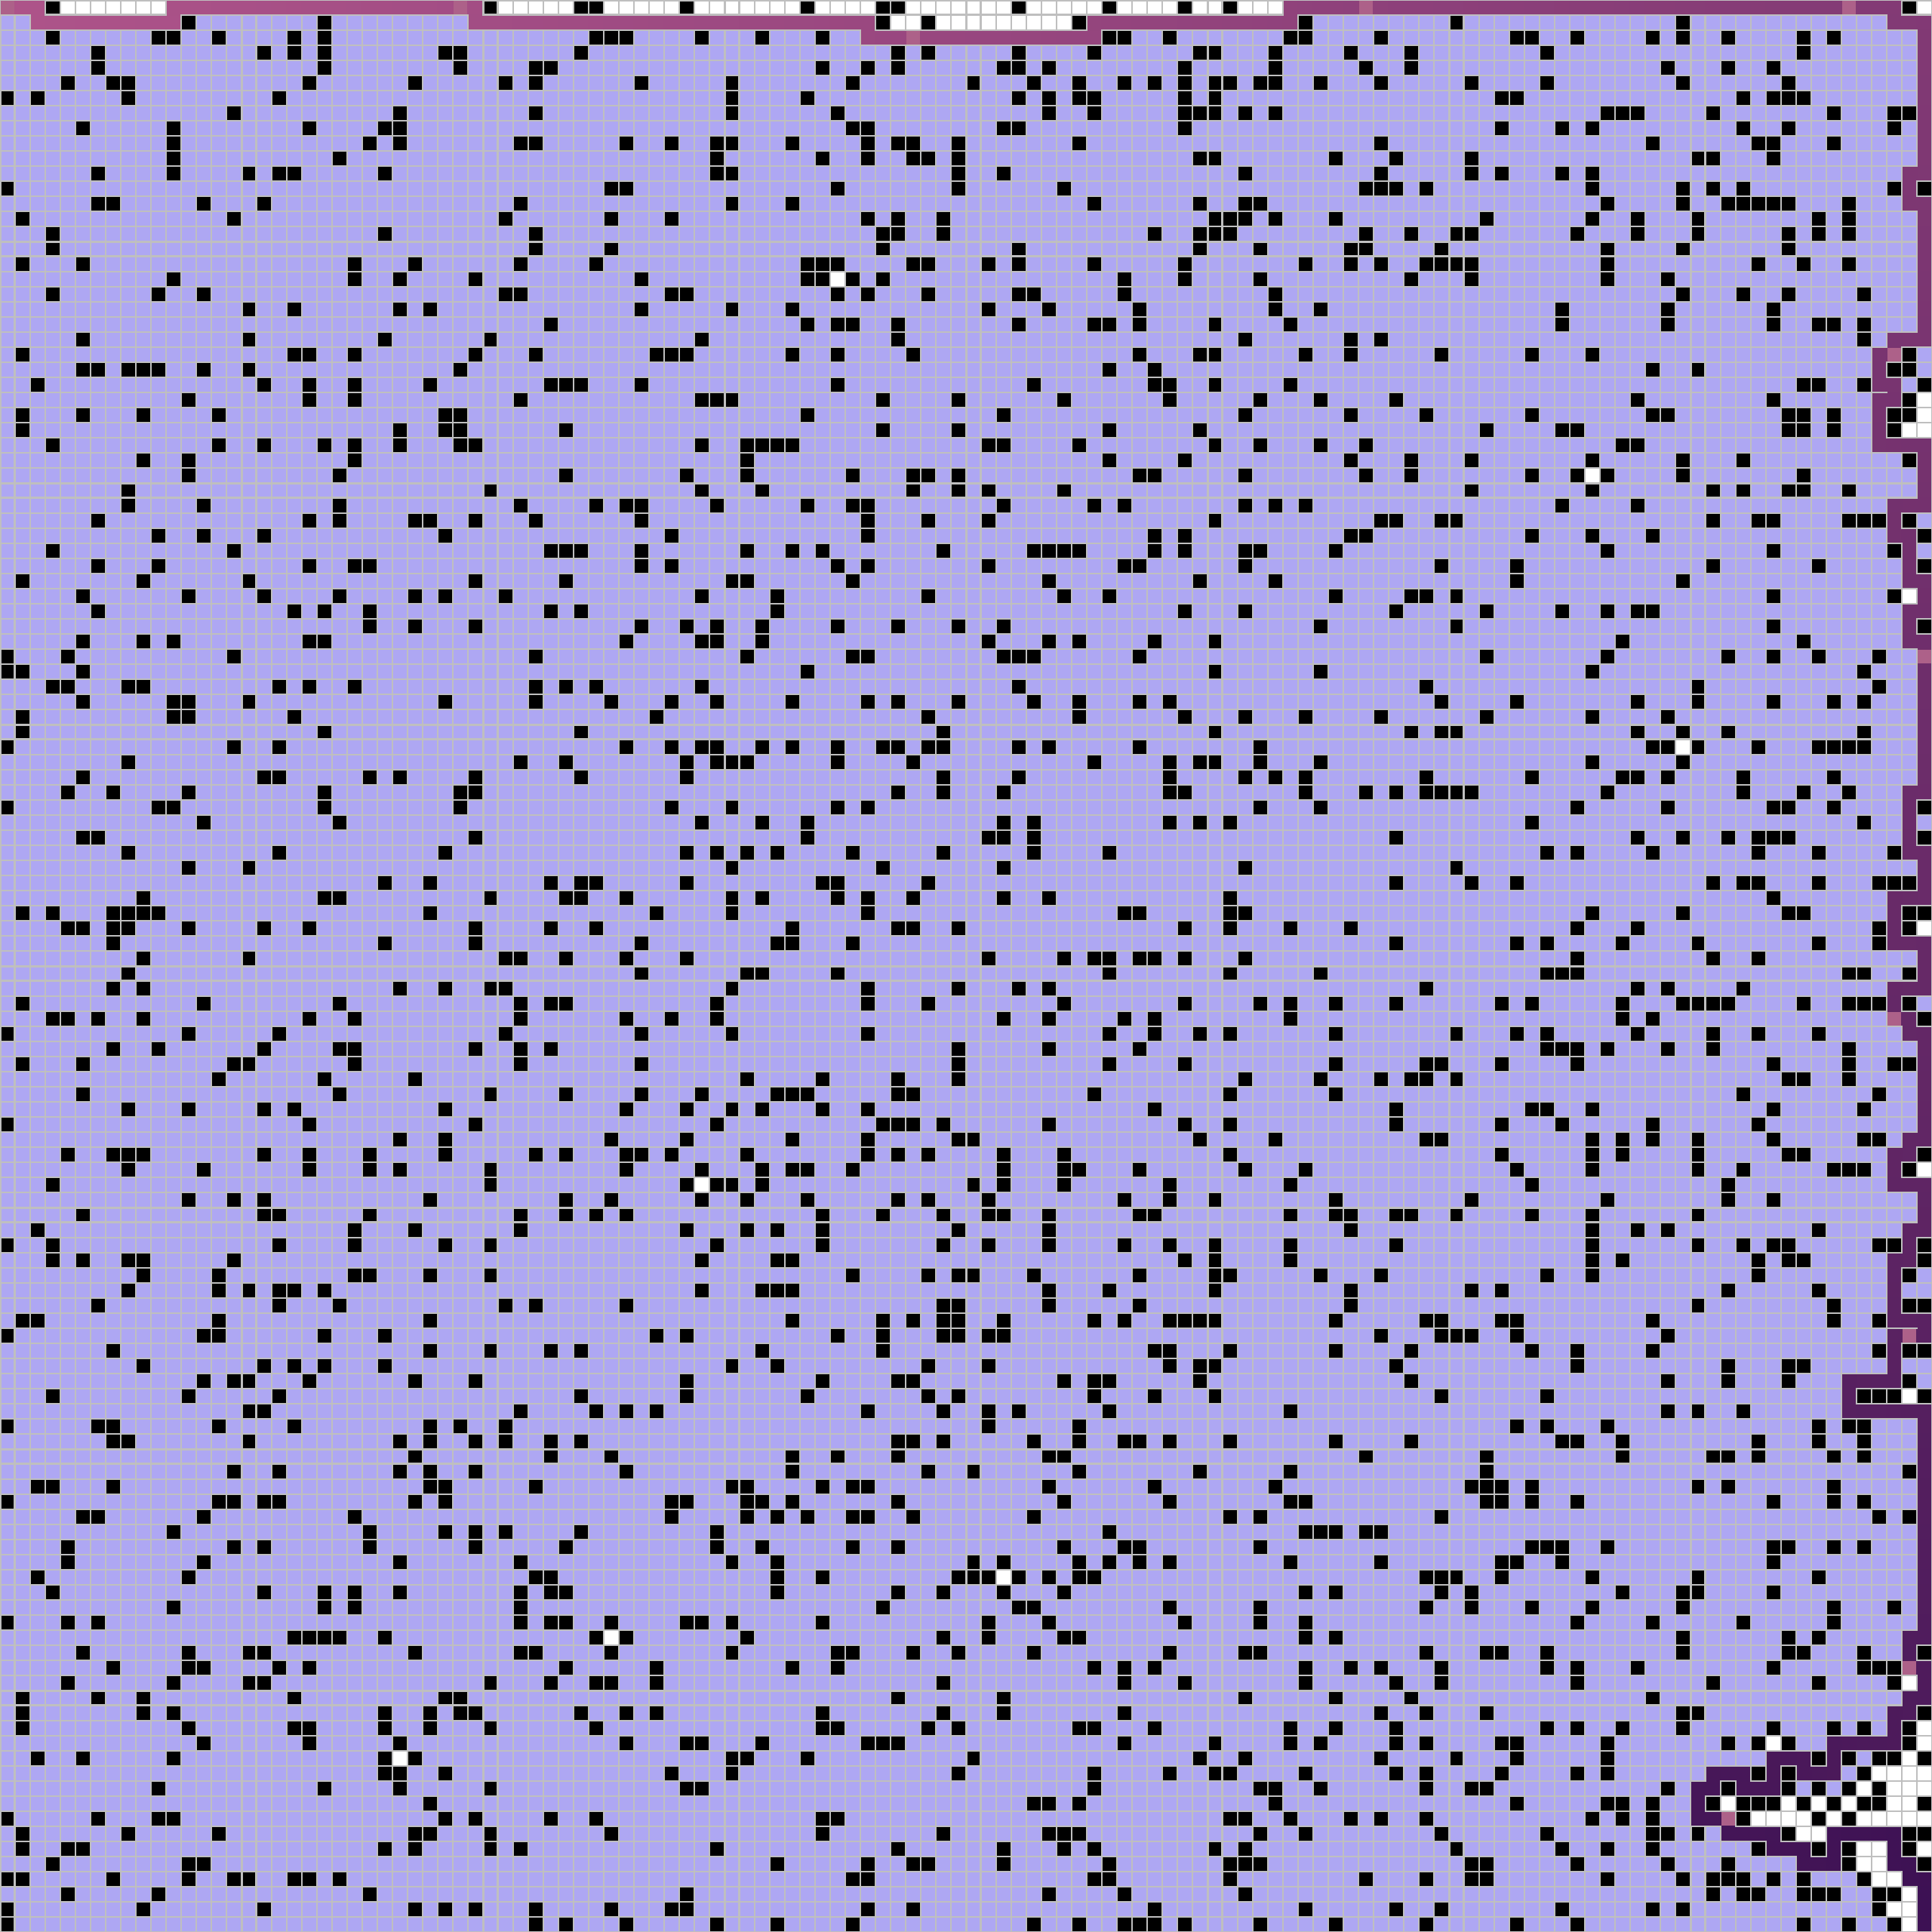
\includegraphics[width=\textwidth]{../pics/df/10032.png}
					\caption{\label{fig:df2}A maze that is hard for BFS in terms of space complexity, whose maximum fringe size is 10032. }
					\endminipage\hfill
					\minipage{0.49\textwidth}
					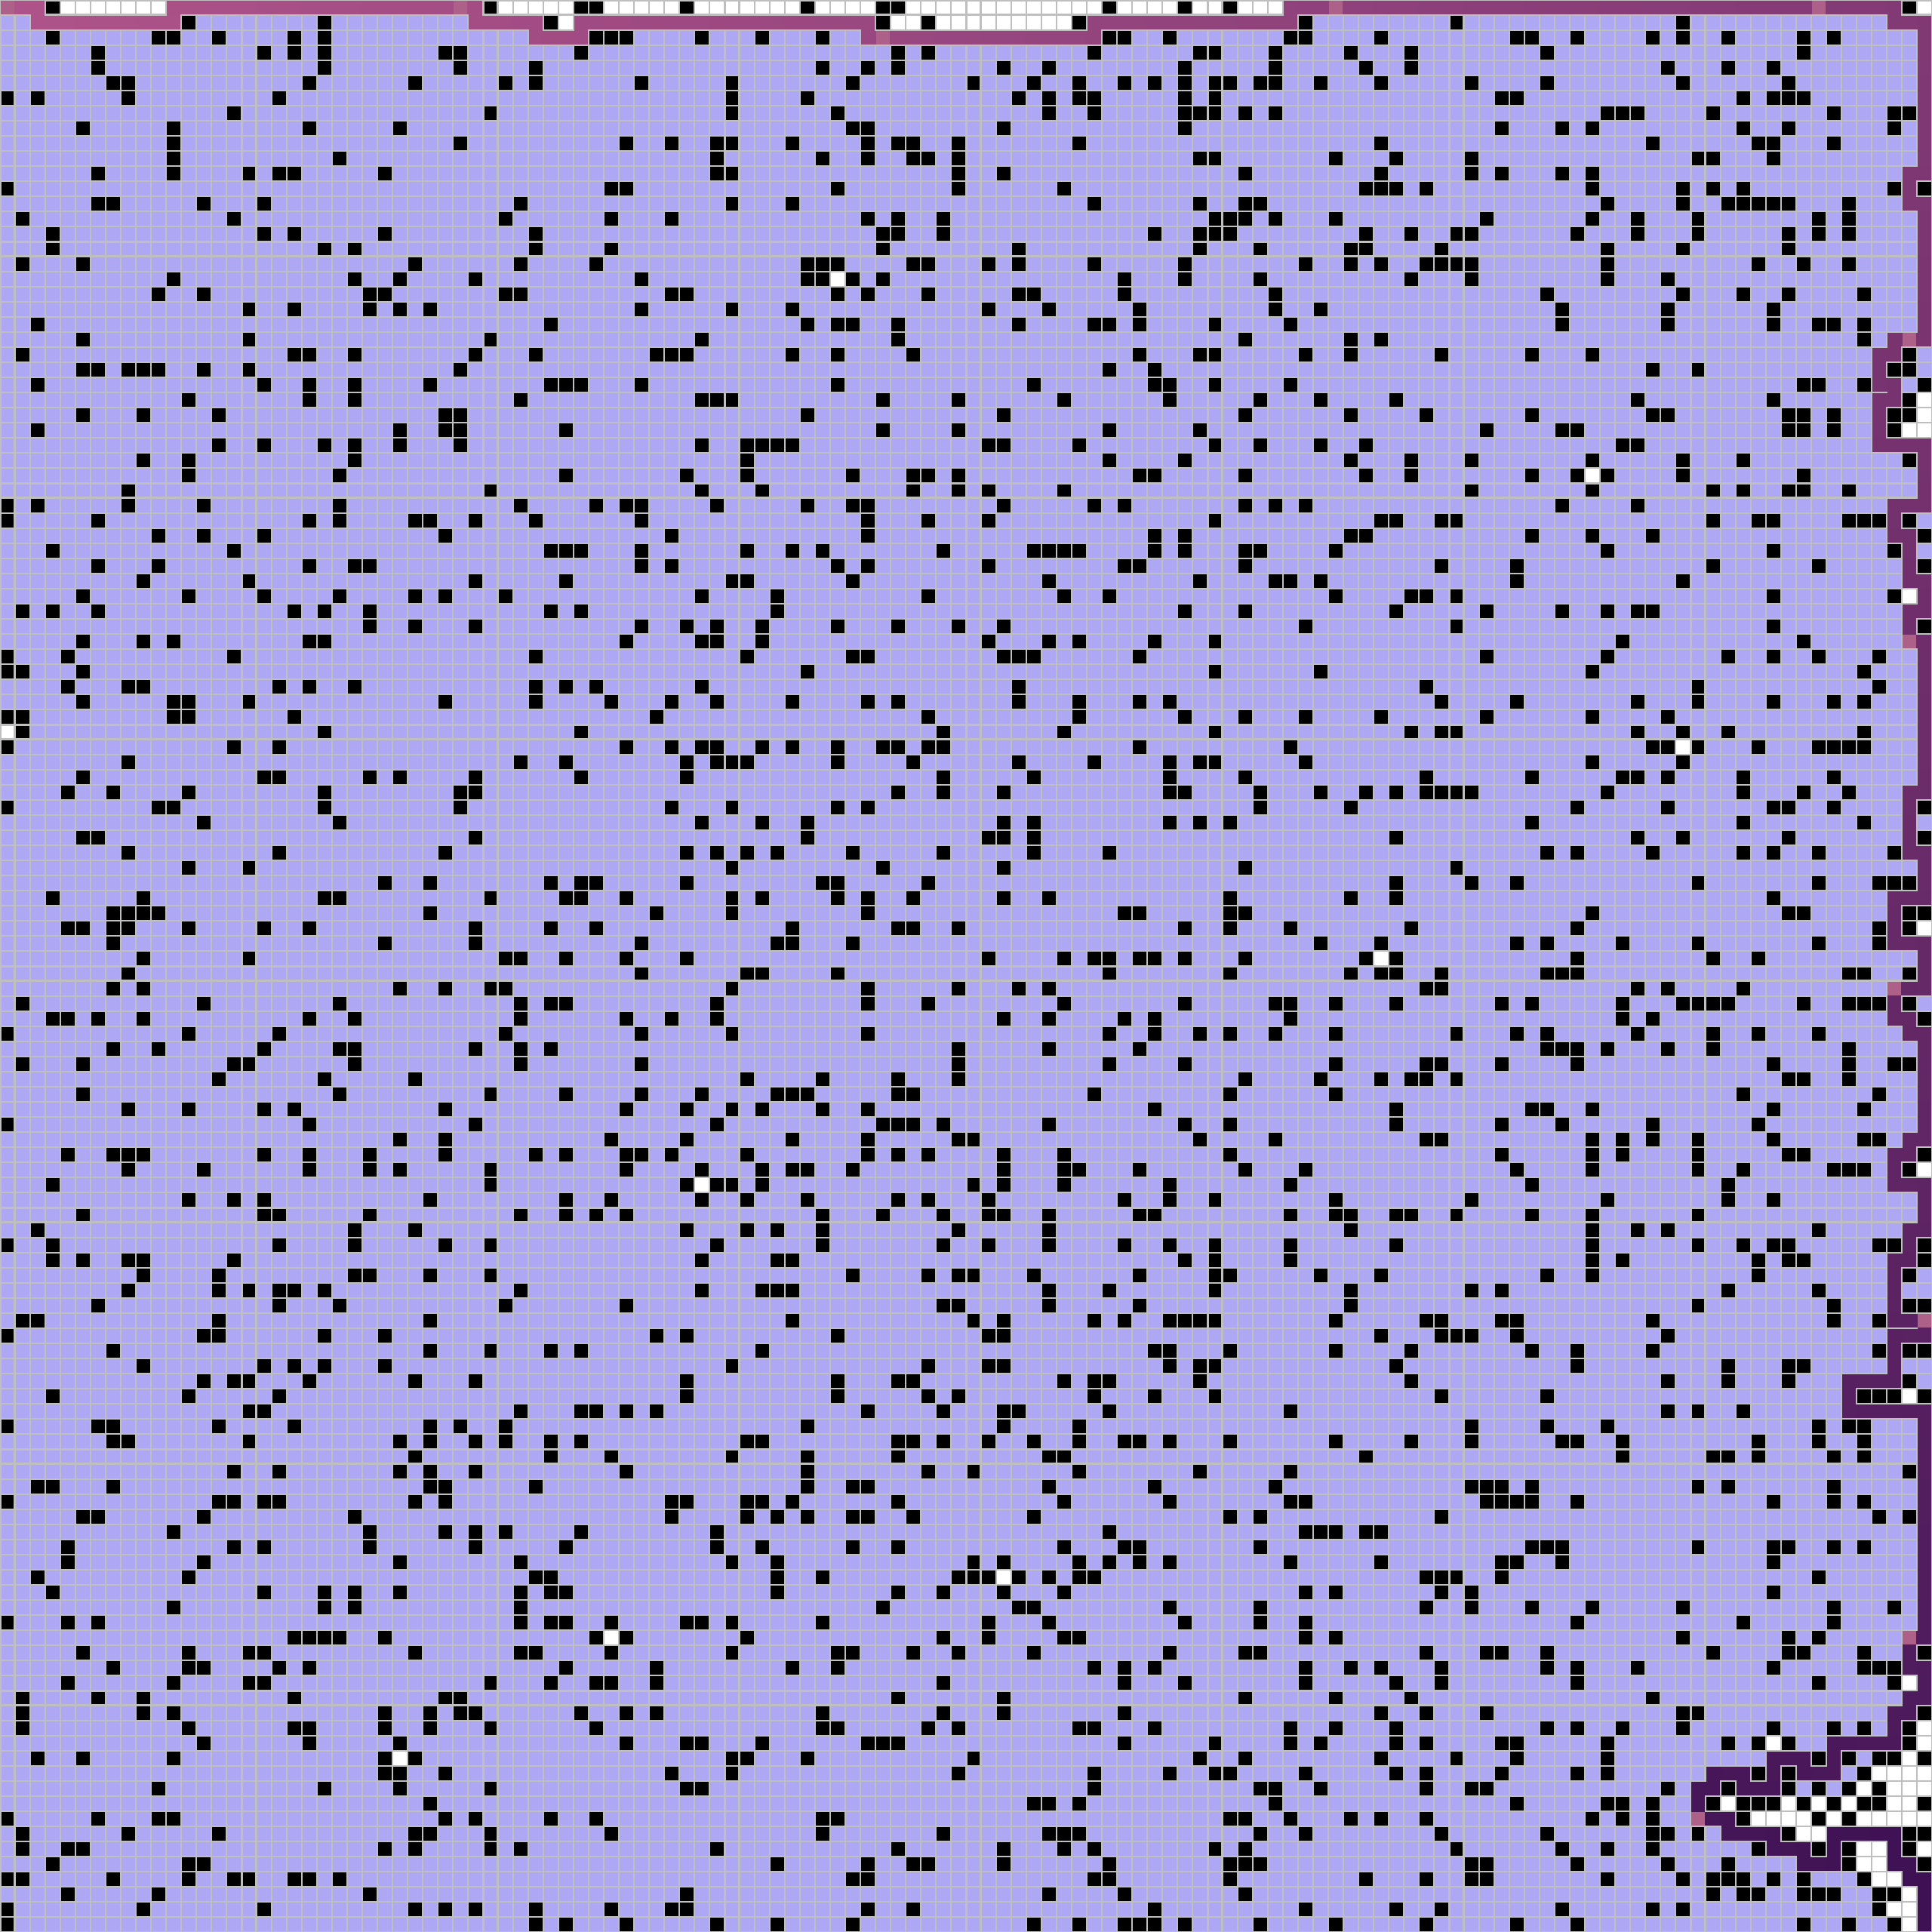
\includegraphics[width=\textwidth]{../pics/df/10031.png}
					\caption{\label{fig:df3} A maze that is hard for BFS in terms of space complexity, whose maximum fringe size is 10031. }
					\endminipage
					\endminipage 
				\end{figure}
				
				\textbf{Patterns or trends:} 
				\begin{itemize}
					\item {The same pattern as Question 10.b.ii, but there should be a clear path along the first row and upper half of the last column.}
				\end{itemize}
				
				\textbf{Reasons:} 
				\begin{itemize}
					\item {The time complexity of DFS related to the maximum depth it has searched.}
					\item {Hence, a "door sill" pattern can force DFS to search lower left part rather than immediately reach the Goal, which increased the maximum depth of DFS.}
					\item {A larger lower left part increases the depth, so the upper right part should be as small as possible.}
				\end{itemize}
				
				\textbf{"The hardest" maze:} 
				\begin{itemize}
					\item {The same maze as Question 10.b.ii.}
					\item {The maximum fringe size is theoretically $(size-1)^2-WallCost = 16113$, compared with 10032. Noticed distinctFringe actually do not promise all elements in the fringe are distinct because it takes too much time to search in a stack frequently. (Further information is available in description.md)}
					\item {Again, it is really difficult to cancel out those outside walls by random without destroying the pattern. Therefore, it has been a nearly "hardest" maze.}
				\end{itemize}
			\end{enumerate}
			
			\item {$ A^* $ with Euclidean Distance Heuristic}
			\label{A*E} 
			\begin{enumerate}
				\item {Length of solution path returned: See Figure \ref{fig:dp1}, Figure \ref{fig:dp2} and Figure \ref{fig:dp3}.} \\
				\begin{figure}
					\minipage{\textwidth}
					
					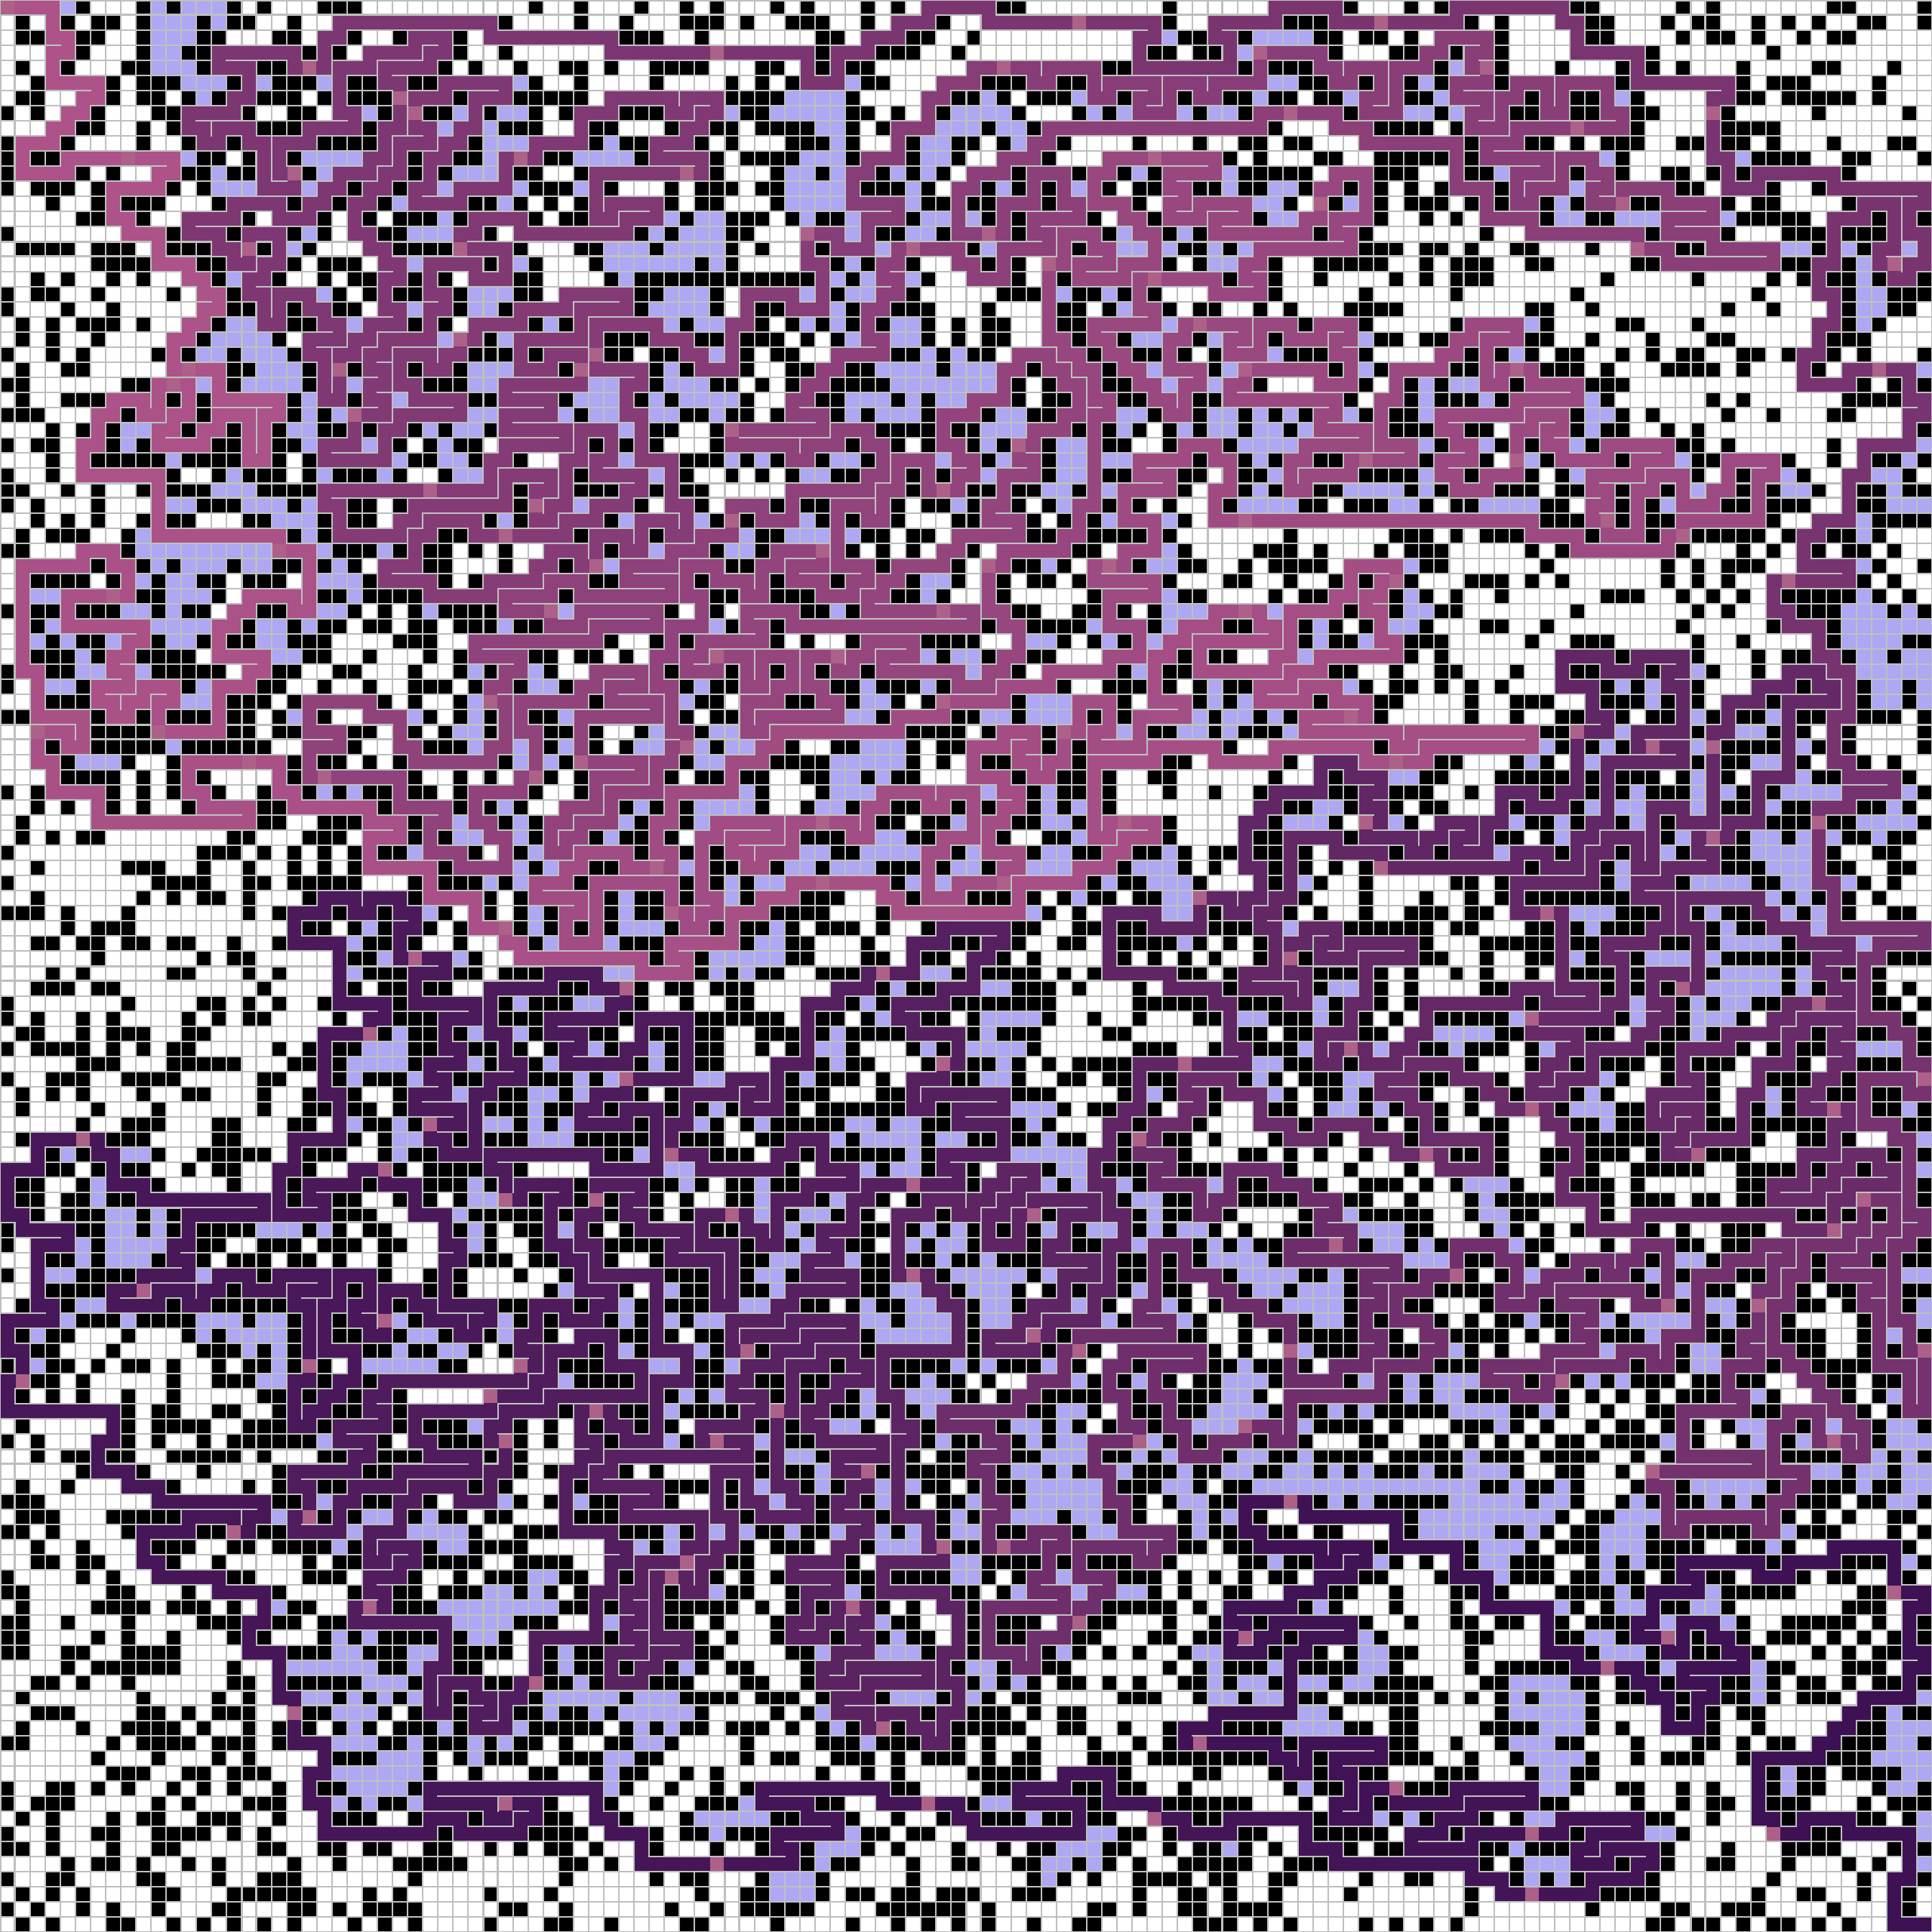
\includegraphics[width=\textwidth]{../pics/dp/5557.png}
					\caption{\label{fig:dp1}maze that is hard for DFS in terms of path length, which is 5557.}
					
					\minipage{0.49\textwidth}
					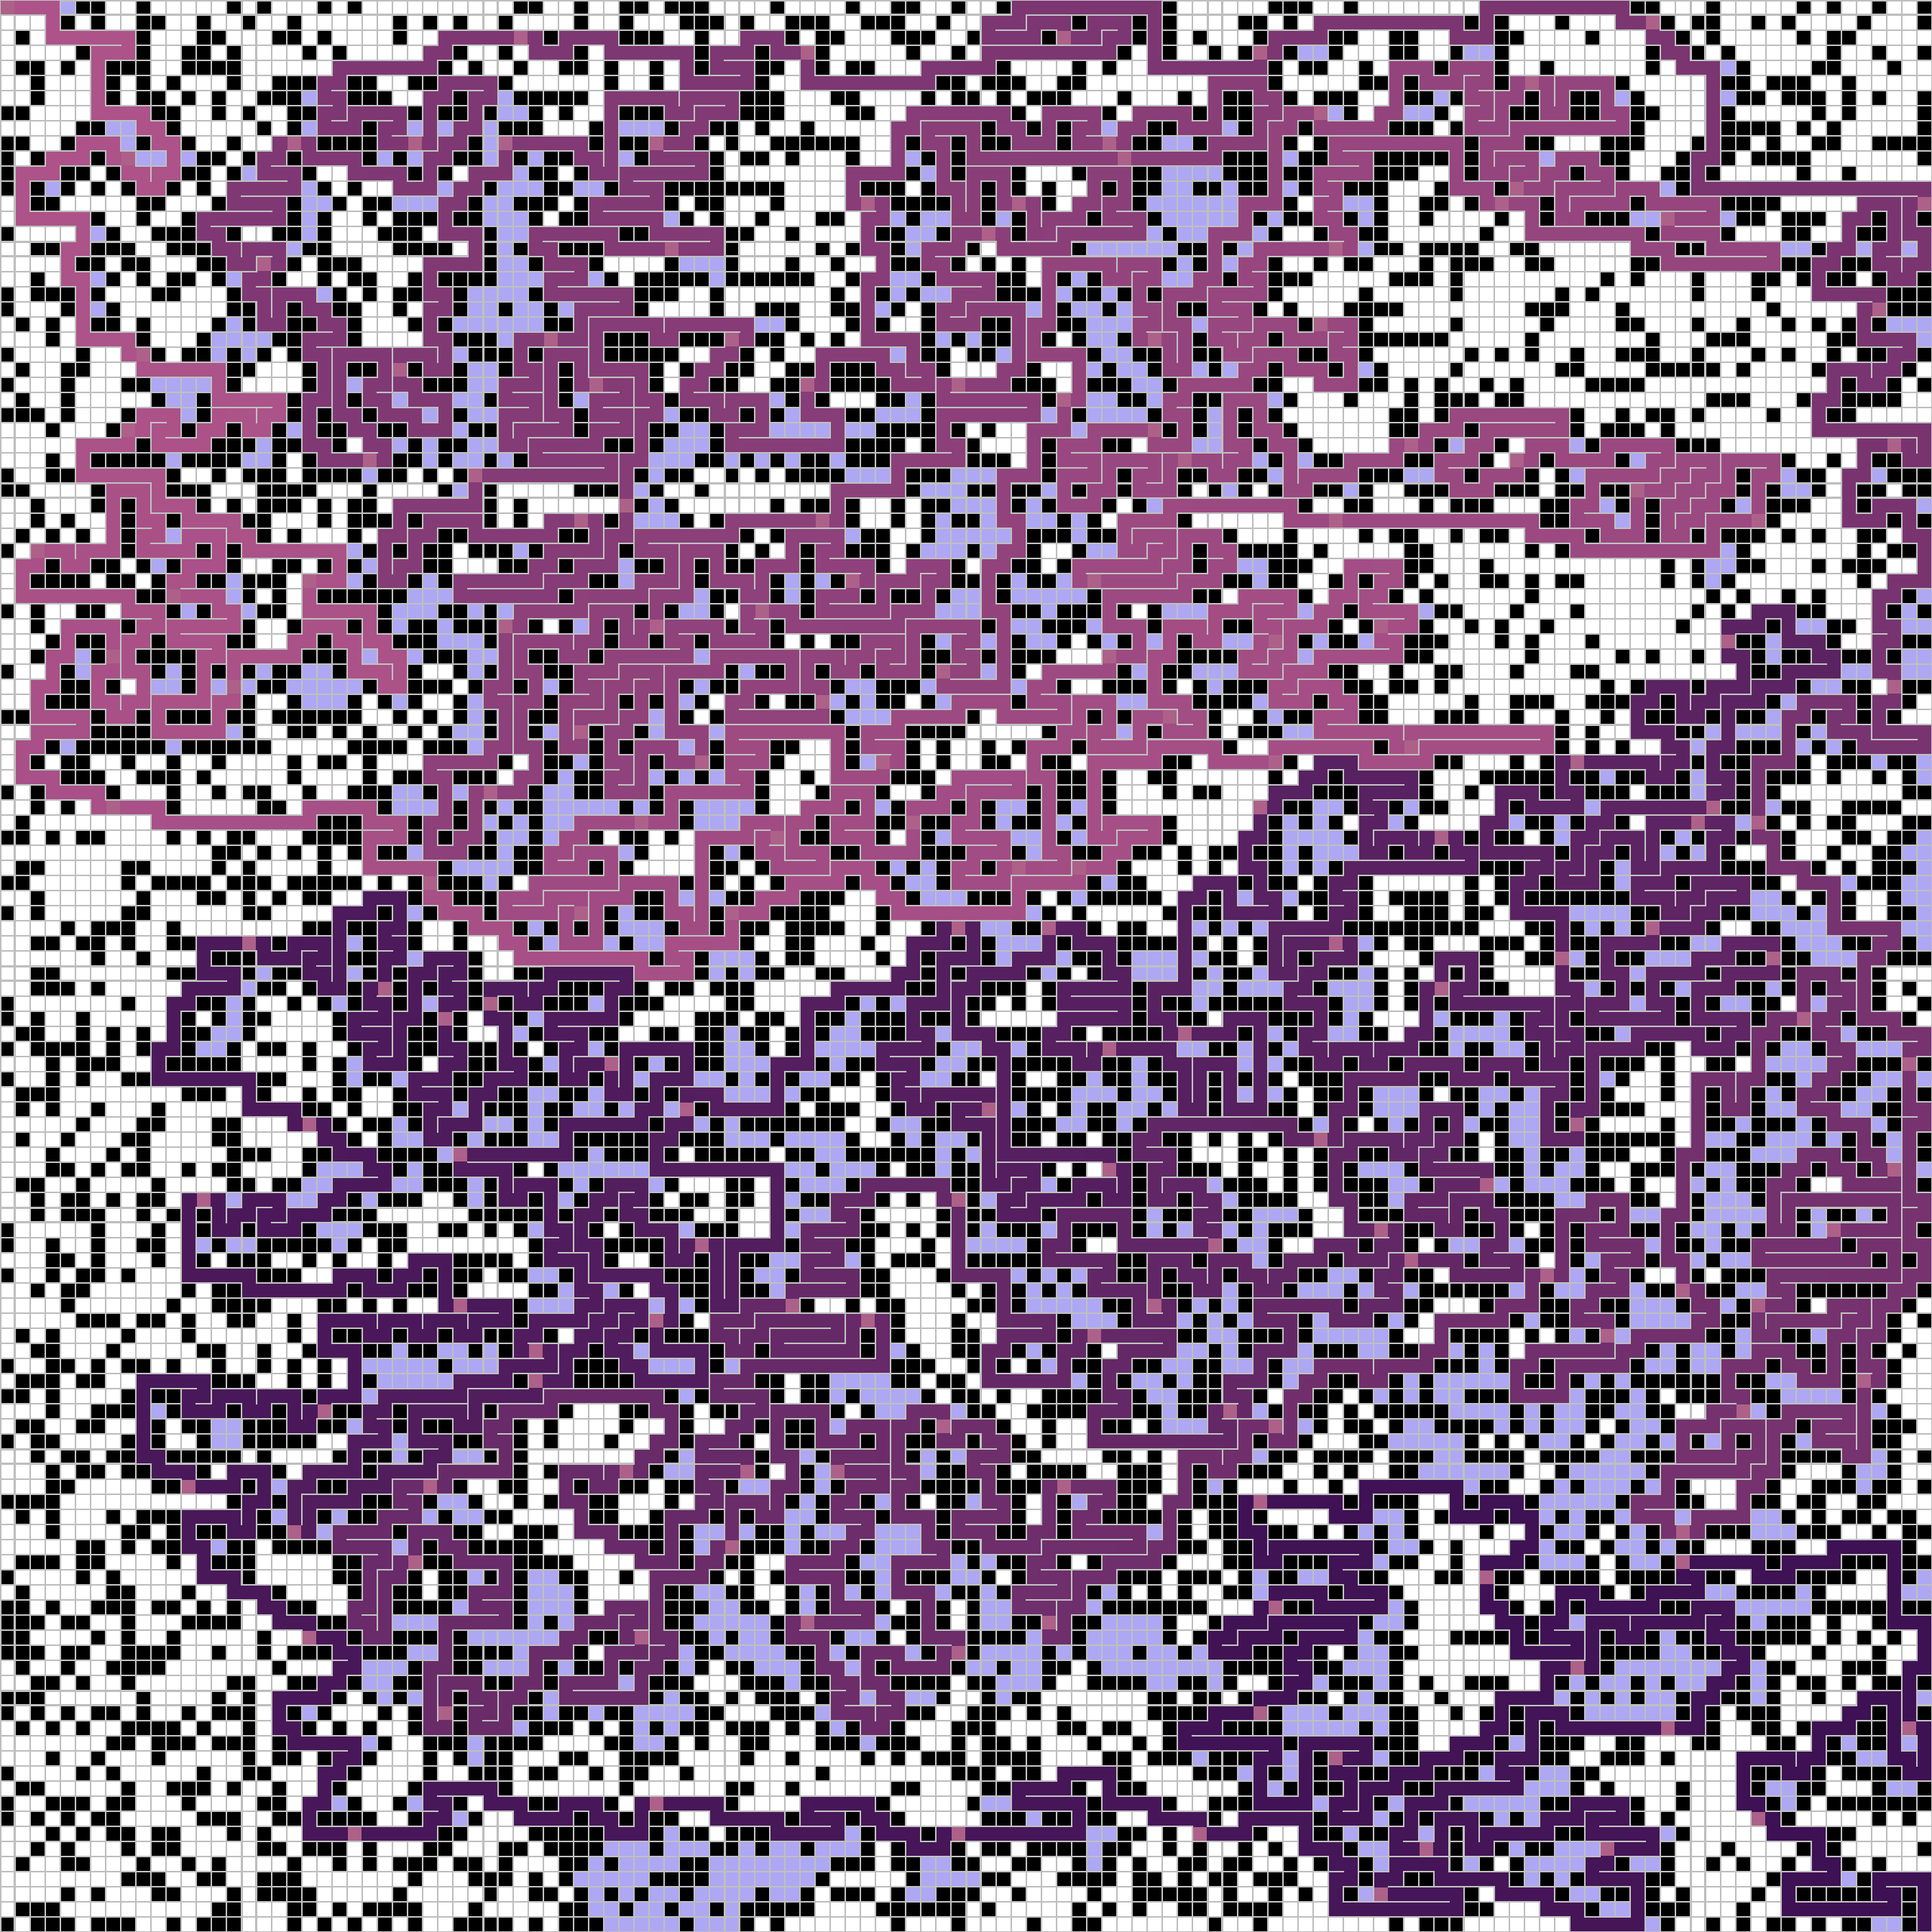
\includegraphics[width=\textwidth]{../pics/dp/5503.png}
					\caption{\label{fig:dp2}maze that is hard for DFS in terms of path length, which is 5503.}
					\endminipage\hfill
					\minipage{0.49\textwidth}
					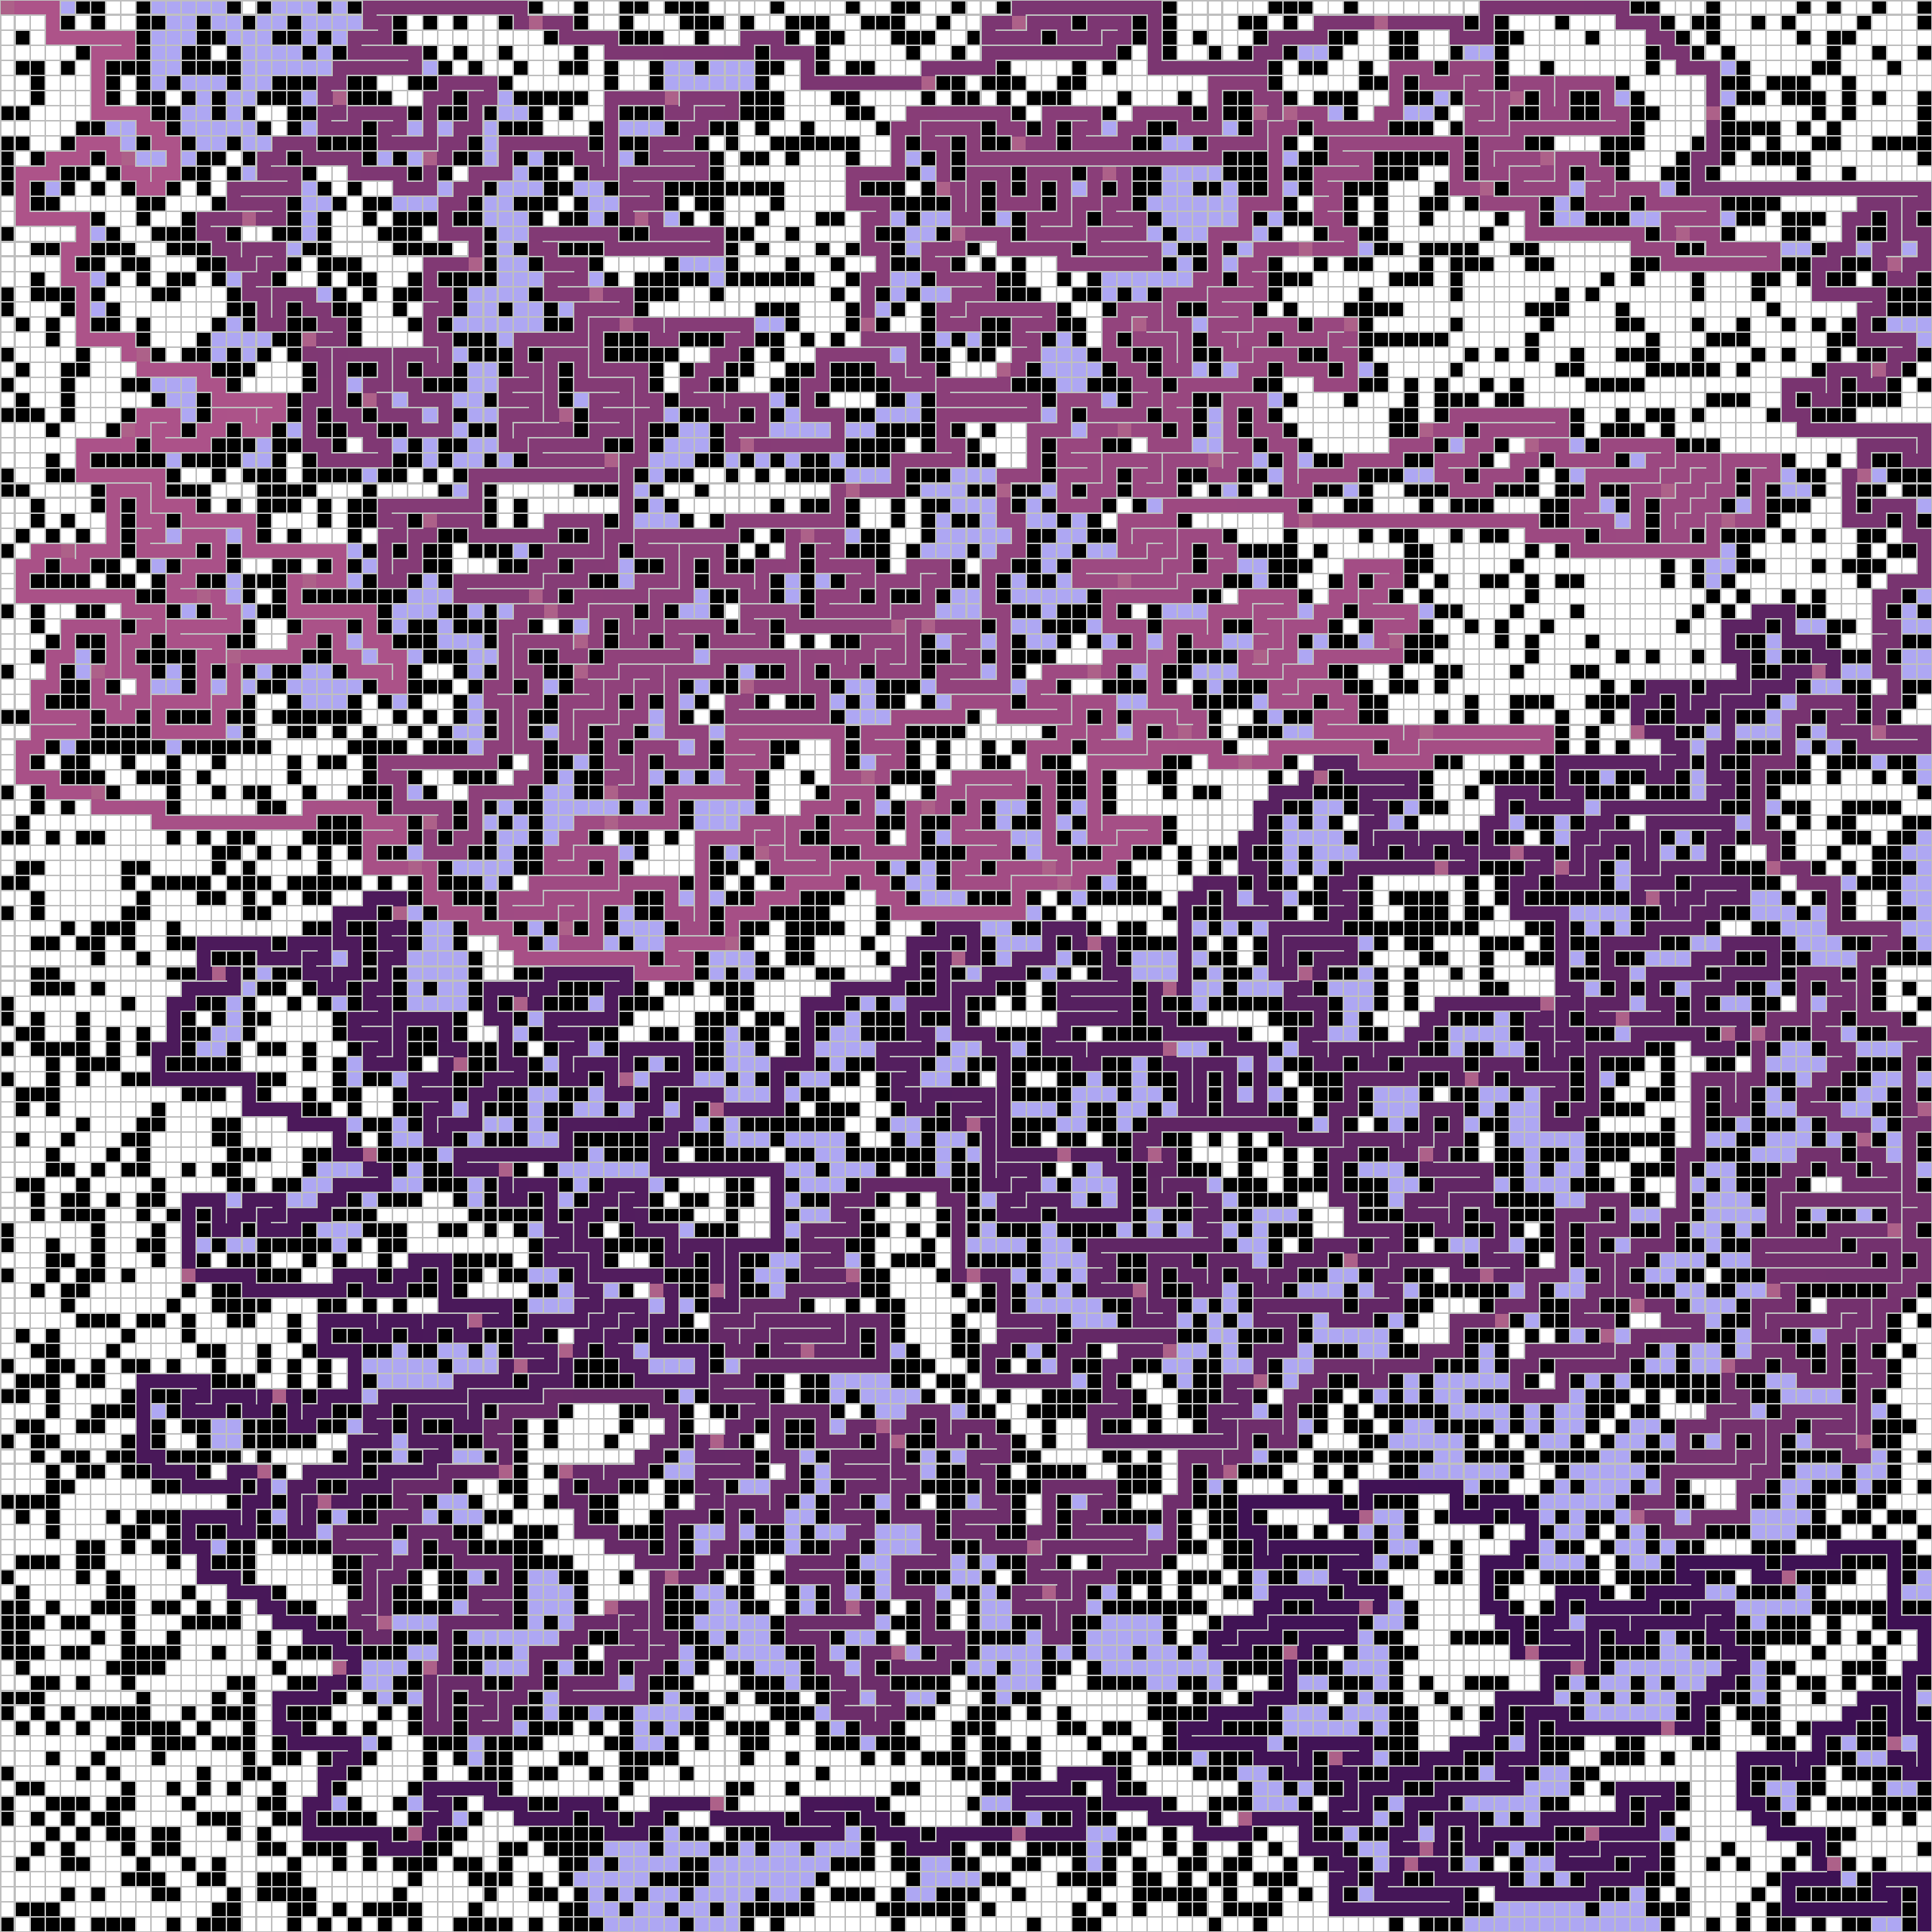
\includegraphics[width=\textwidth]{../pics/dp/5495.png}
					\caption{\label{fig:dp3}maze that is hard for DFS in terms of path length, which is 5495.}
					\endminipage
					\endminipage
					
				\end{figure}
				\textbf{Patterns or trends:} 
				\begin{itemize}
					\item {There are 2 classical patterns of walls. (See Figure \ref{fig:dp-pattern}) In one case, walls lead agents to go down some rows, then there usually several nearly "empty"(no walls) rows to move horizontally. But at the end of these rows, diagonal walls lead agents to move up. This case looks like "I" and ">". The other case is "J-shape" walls. }
					\begin{figure}
						\minipage{0.6\textwidth}
						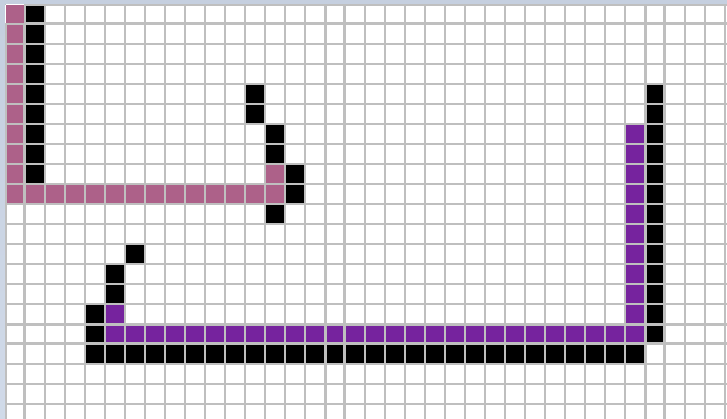
\includegraphics[width=\textwidth]{../pics/dp/pattern.png}
						\caption{\label{fig:dp-pattern}Two classical patterns of walls: "I" and ">" walls and "J-shape" walls.}
						\endminipage\hfill
						\minipage{0.39\textwidth}
						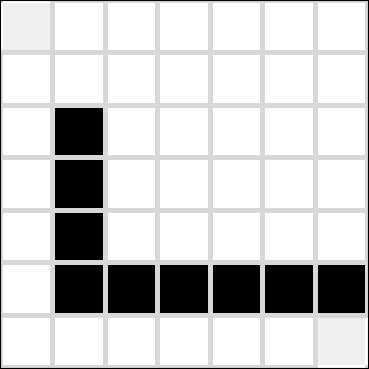
\includegraphics[width=\textwidth]{../pics/dp/hardest.png}
						\caption{\label{fig:dp-hardest}}
						\endminipage
					\end{figure}
					
					\item {"I" and ">" walls and "J-shape" walls appear alternately.}
				\end{itemize}
				
				\textbf{Reasons:} 
				\begin{itemize}
					\item {The key point is when randomWalk == False, the priority of 4 directions is Right > Down > Left > Up.}
					\item {"I" and ">" walls lead agent walk horizontally, and the path it has walked becomes "new wall" because those blocks have been added into the closed set. Now it becomes a "J-shape" walls in the mirror.}
					\item {"J- shape" walls force agents search all blocks inside because agents prefer to go right or left than to move up.}
				\end{itemize}
				
				\textbf{"The hardest" maze:} 
				\begin{itemize}
					\item {The ideal "J-shape" walls can be maze-sized. (See Fig \ref{fig:dp-hardest}) In this case, the path length can be $size \times size - WallCost = 16312$. Notice that if size is an odd number, not all the accessible blocks are in the path. Specifically, only the first 3 blocks in the 2nd row are in the path. }
					\item {Compared with 16312, 5557 is not a big number. However, it is extremely impossible to randomly set all walls in a line.}
					\item {However, compared with less than 1000 block length in a 200 by 200 maze(from Question 5), 5557 in a 128 by 128 maze can be regarded as a "harder" maze, though it is not the "hardest" maze.}
				\end{itemize}
				
				\item {Total number of nodes expanded: See Figure \ref{fig:dp1}, Figure \ref{fig:dp2} and Figure \ref{fig:dp3}.} \\
				\begin{figure}
					\minipage{\textwidth}
					
					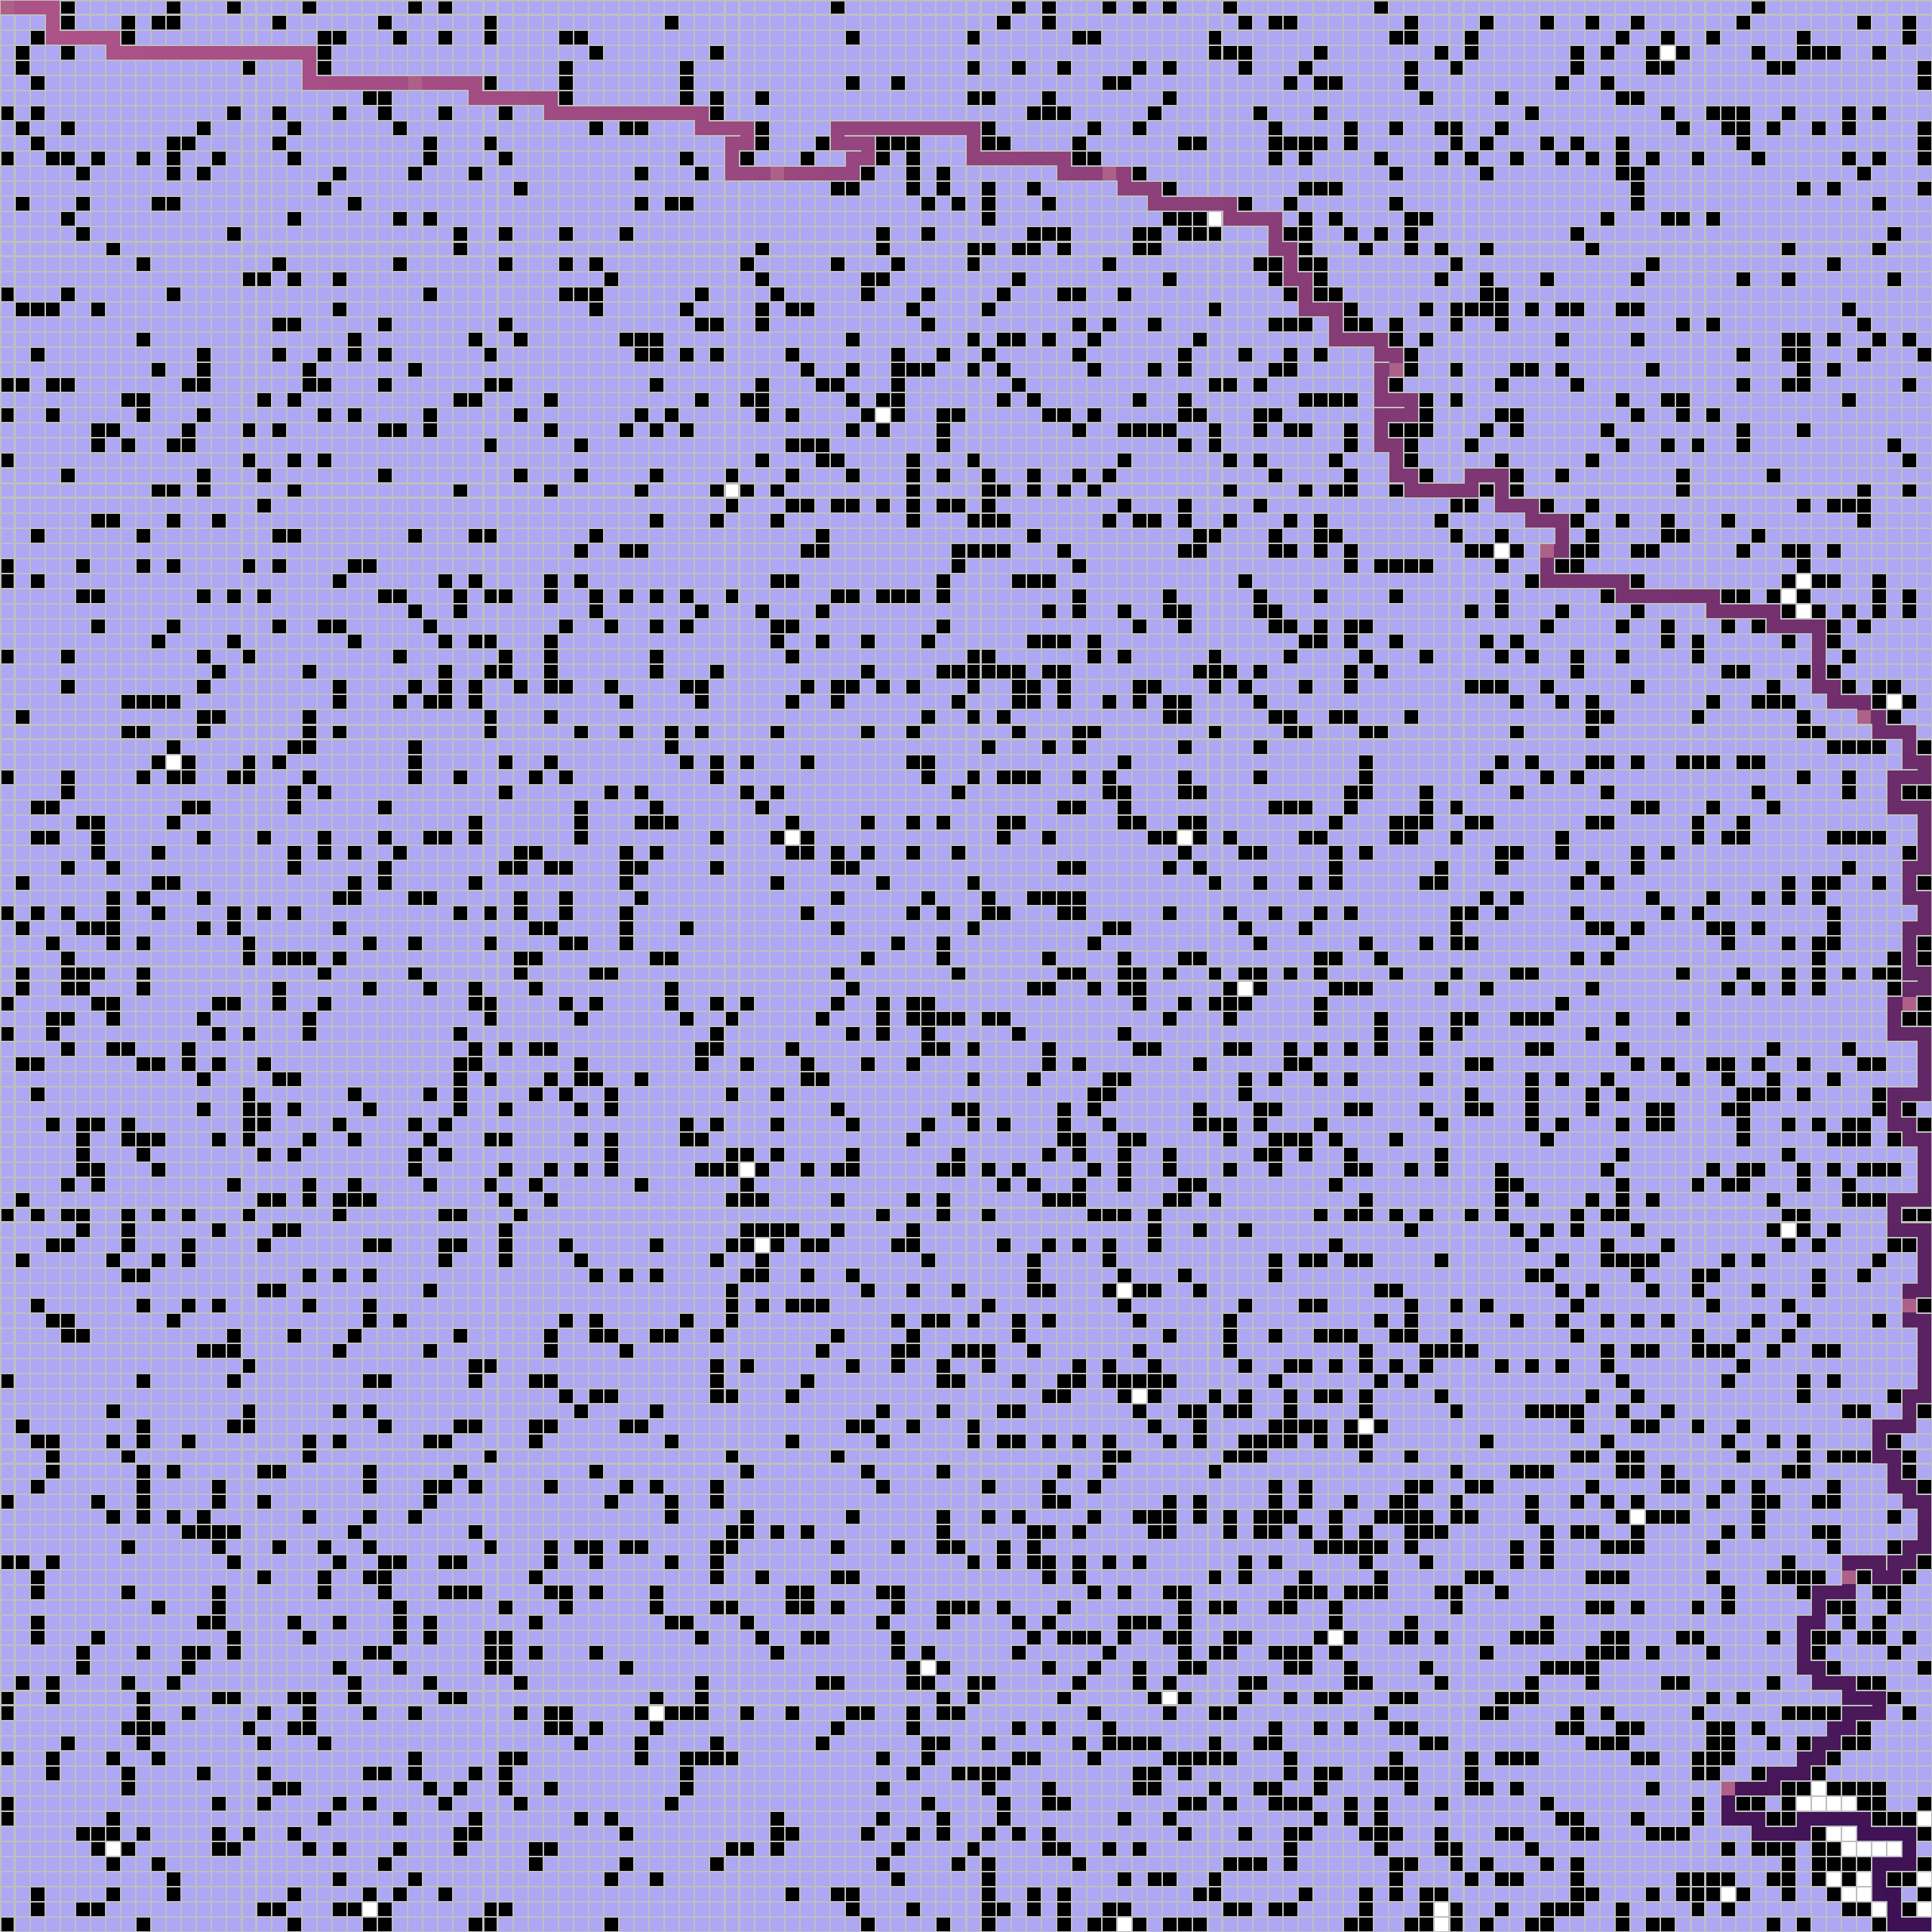
\includegraphics[width=\textwidth]{../pics/db/12993.png}
					\caption{\label{fig:db1}A maze that is hard for DFS in terms of time complexity, which has opend 12993 blocks.}
					
					\minipage{0.49\textwidth}
					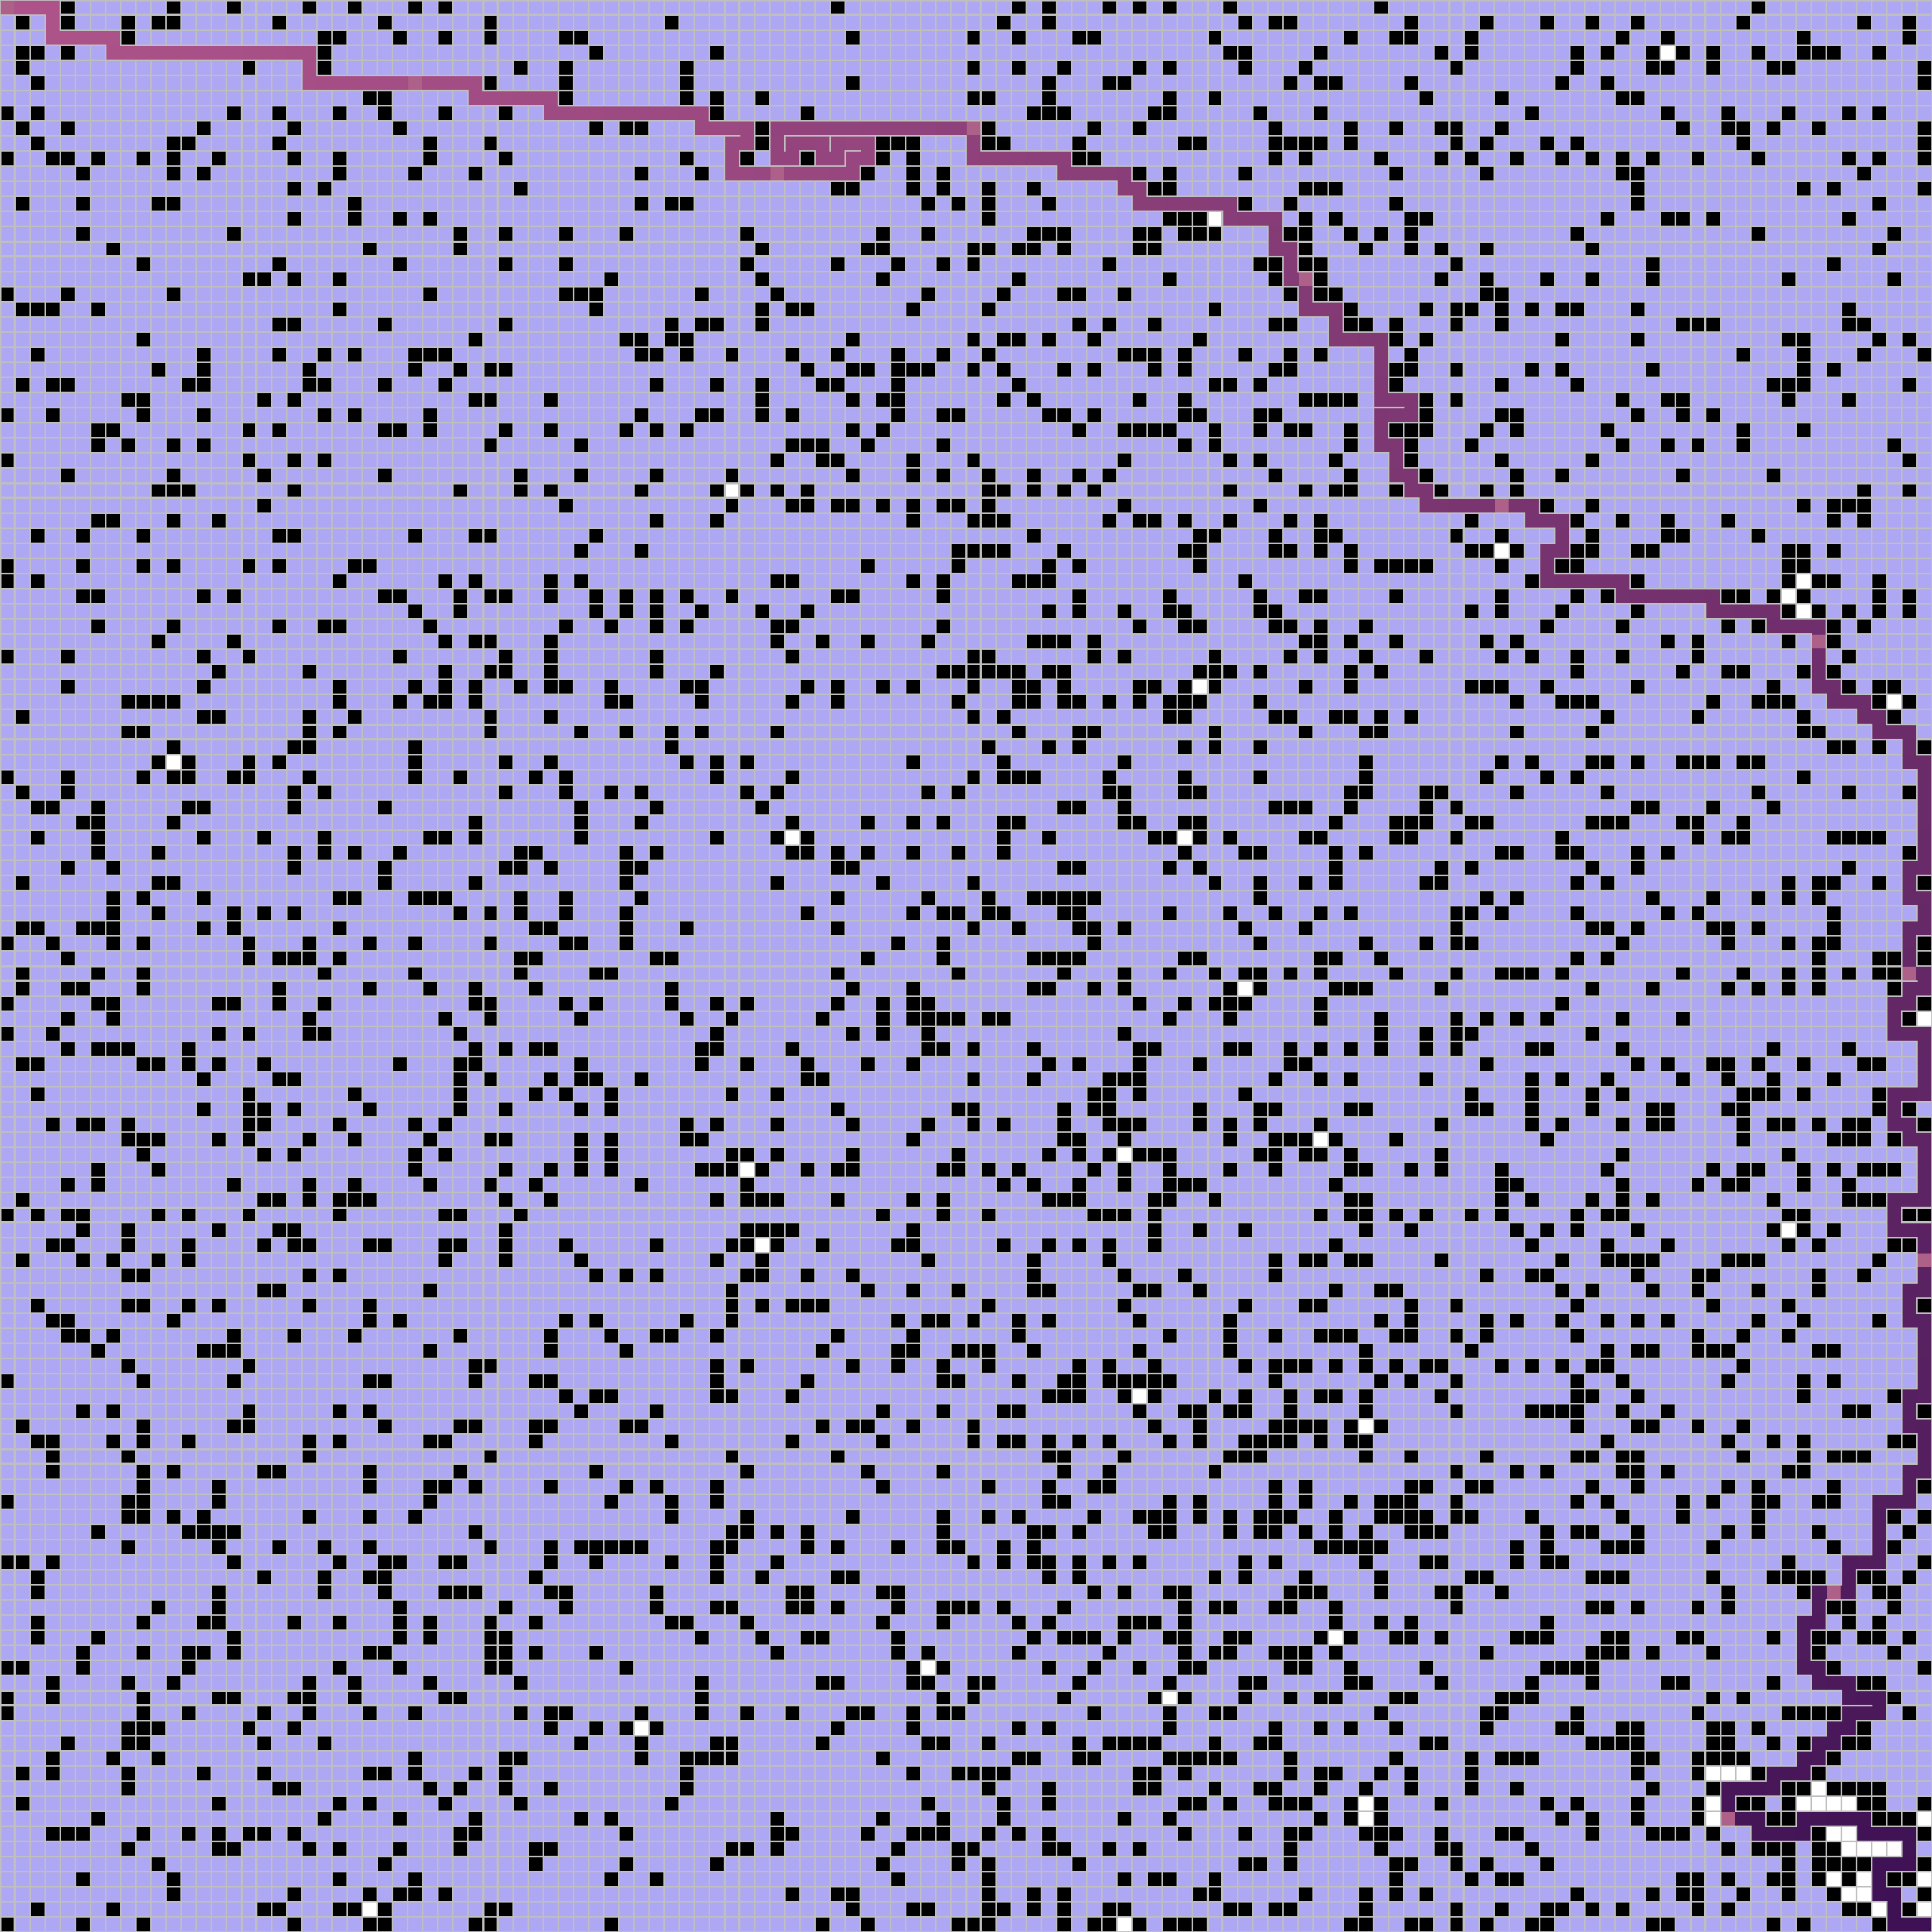
\includegraphics[width=\textwidth]{../pics/db/12968.png}
					\caption{\label{fig:db2}A maze that is hard for DFS in terms of time complexity, which has opend 12968 blocks.}
					\endminipage\hfill
					\minipage{0.49\textwidth}
					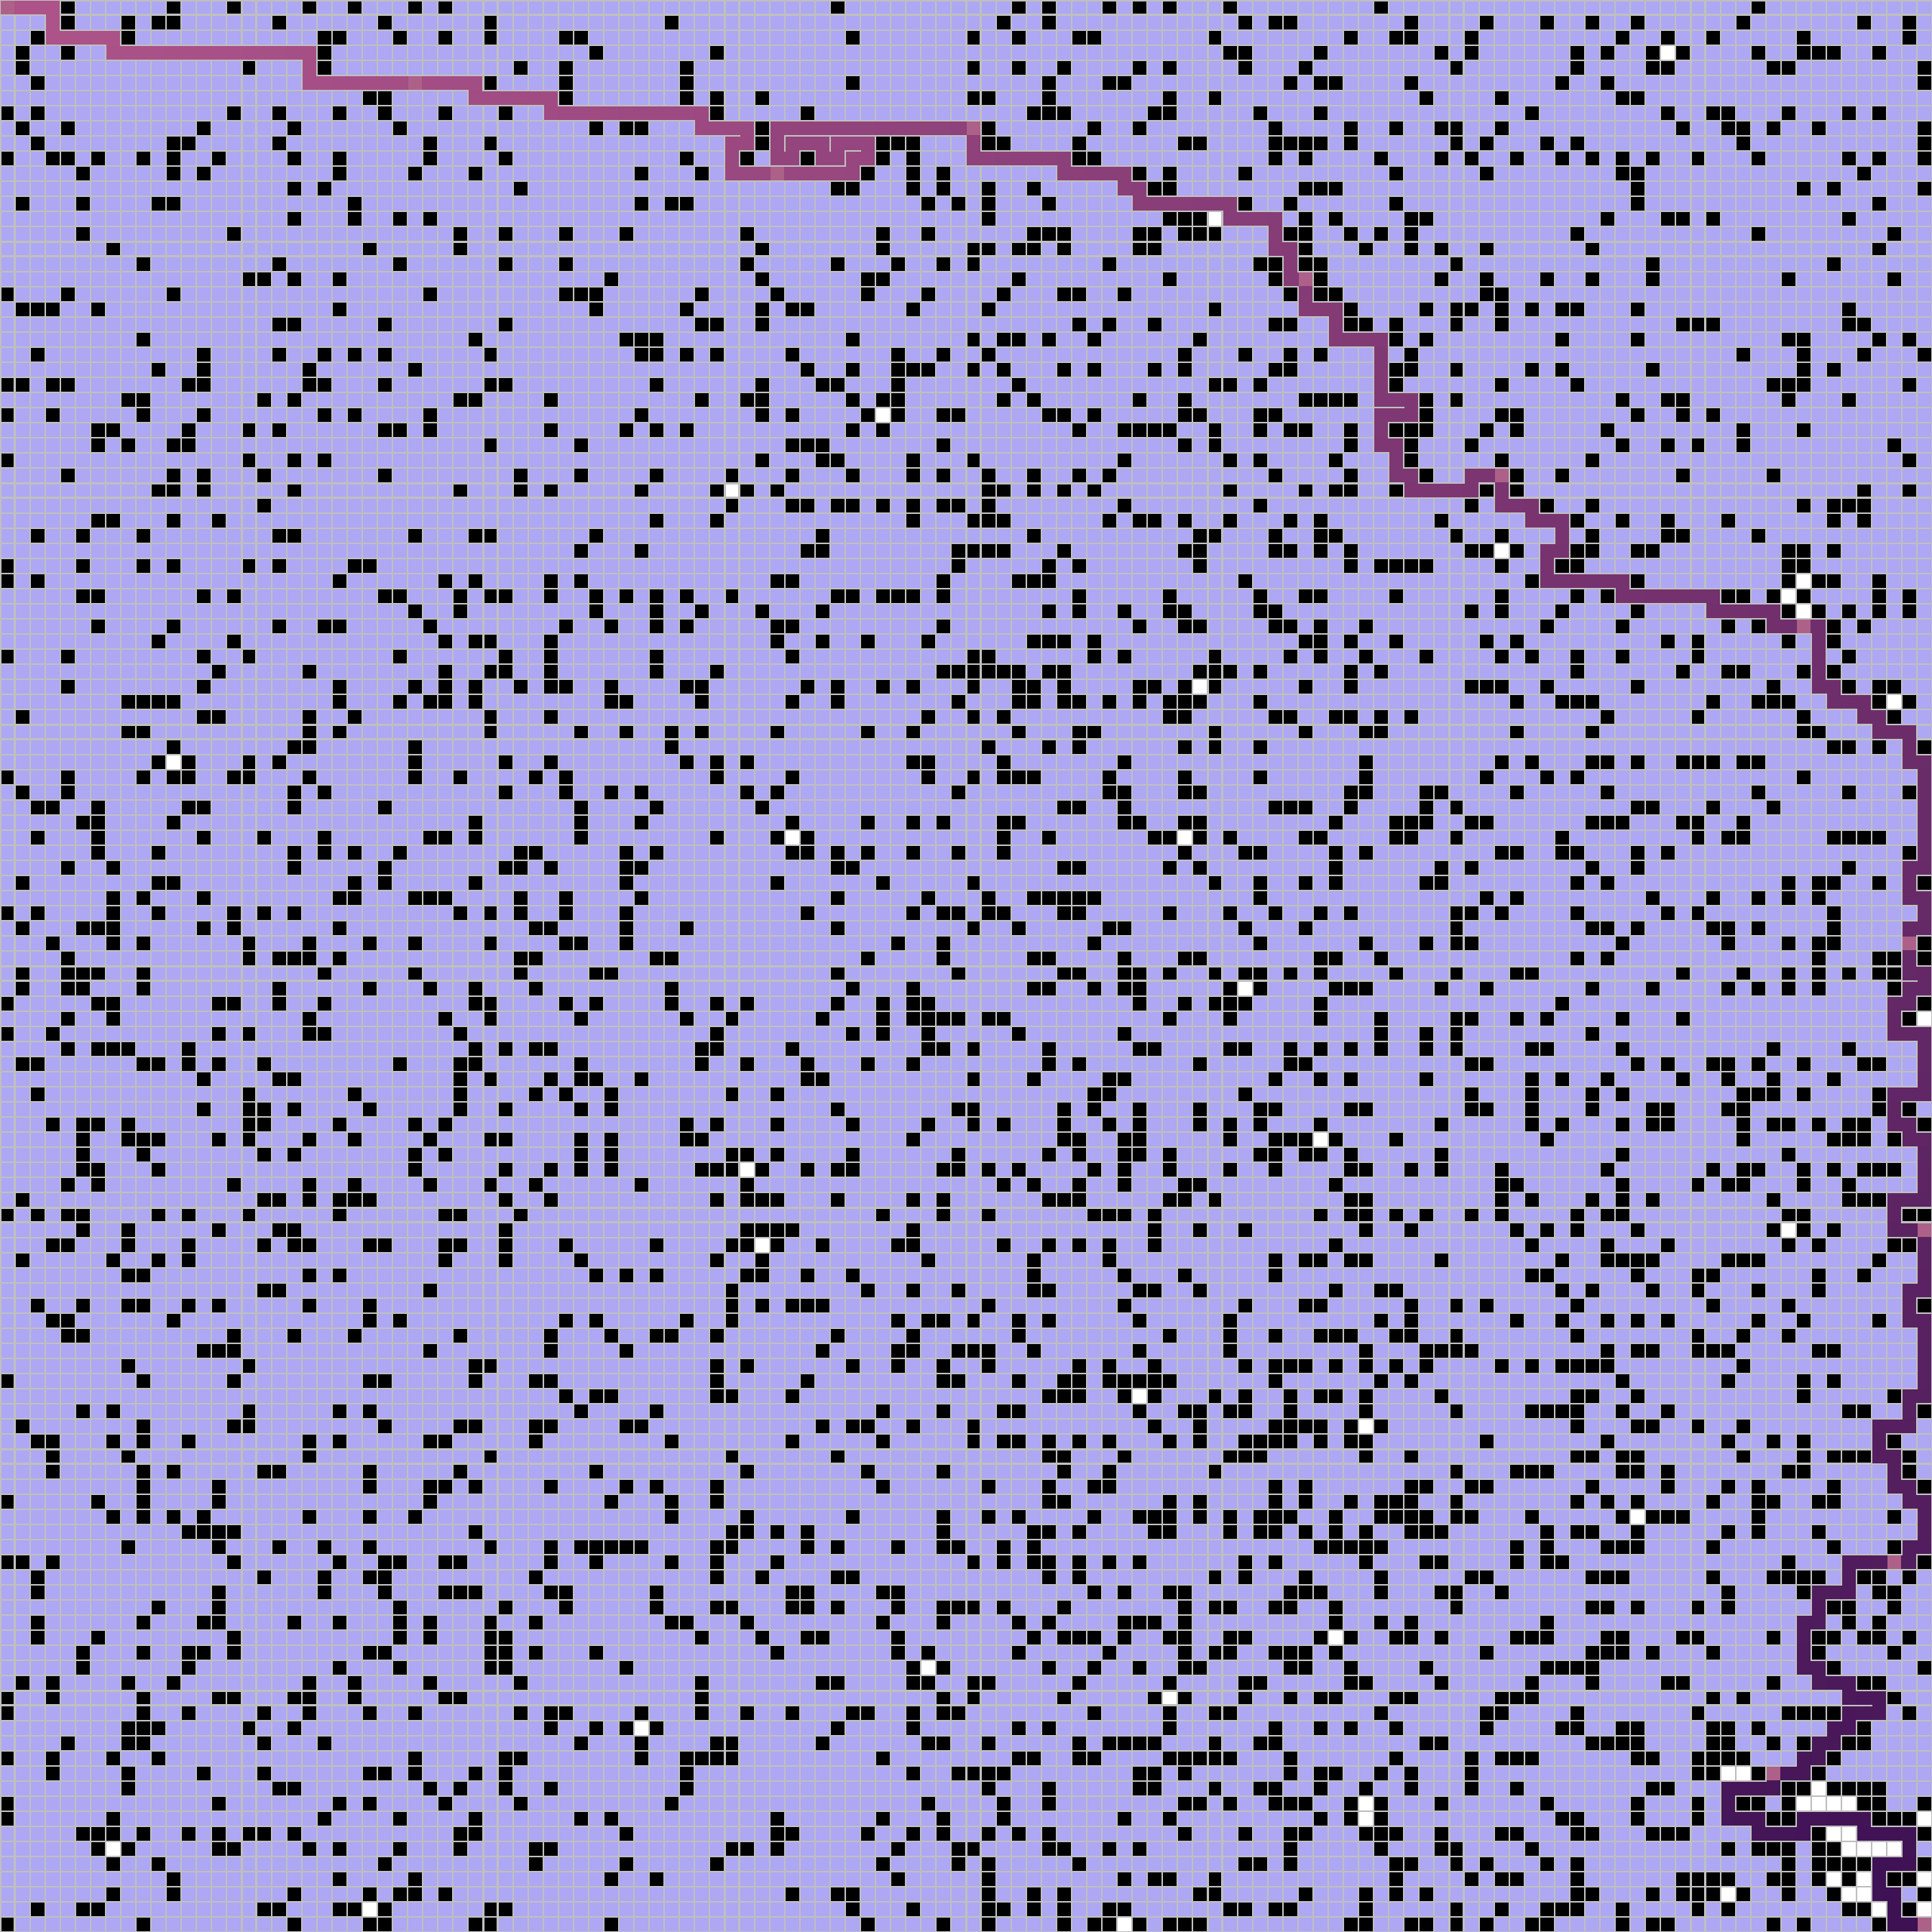
\includegraphics[width=\textwidth]{../pics/db/12967.png}
					\caption{\label{fig:db3} A maze that is hard for DFS in terms of time complexity, which has opend 12967 blocks.}
					\endminipage
					\endminipage 
				\end{figure}
				
				\textbf{Patterns or trends:} 
				\begin{itemize}
					\item {The pathway near the Goal(10 * 10 blocks in the lower right corner) is extremely narrow(only 1 block width), opens to left, and begins with a "door sill" wall that forces the path to move up a block.}
					
					\item {"I" and ">" walls and "J-shape" walls appear alternately.}
				\end{itemize}
				
				\textbf{Reasons:} 
				\begin{itemize}
					\item {Notice that when randomWalk == False, the priority of 4 directions is Right > Down > Left > Up.}
					\item {The pathway opens to left rather than up makes DFS cannot first run right to the last column and then find the pathway. It takes time for DFS to search all upper right part(above the path) and then realize "Oops, there is no way to the goal. I have to backtrack."}
					\item {After DFS reached the "door sill", it prefers to go to any directions but up. Hence, it takes more time for DFS to search all lower left part(below the path) and then realize "Alright, I will go up to see if there is a path."}
					\item {Therefore, DFS nearly searched all the blocks to reach the Goal.}
					\item {Notice that if randomWalk == True, this pattern will not always work because DFS may go down first rather than right.}
				\end{itemize}
				
				\textbf{"The hardest" maze:} 
				\begin{itemize}
					\item {A maze is "empty"(no walls) except the lower right corner. The lower right corner should be a pathway like this pattern. The smallest pattern can be done in 4 * 4.(See Fig \ref{fig:db-hardest}). Notice there must be at least 2 block height "door sill" for DFS to turn back to search lower left part. }
					\begin{figure}
						\centering
						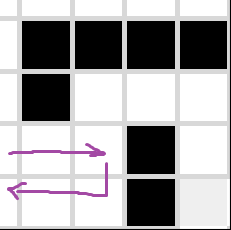
\includegraphics[width=0.3\textwidth]{../pics/db/hardest.png}
						\caption{\label{fig:db-hardest} The smallest pathway pattern.}
					\end{figure}
					\item {Compare to $size \times size - WallCost =16377$, 12993 can still be improved. However, it is really difficult to cancel out those outside walls by random without destroying the pattern. Therefore, it has been a nearly "hardest" maze.}
				\end{itemize}
				
				
				\item {Maximum size of fringe during runtime: See Figure \ref{fig:df1}, Figure \ref{fig:df2} and Figure \ref{fig:df3}.} \\
				\begin{figure}
					\minipage{\textwidth}
					
					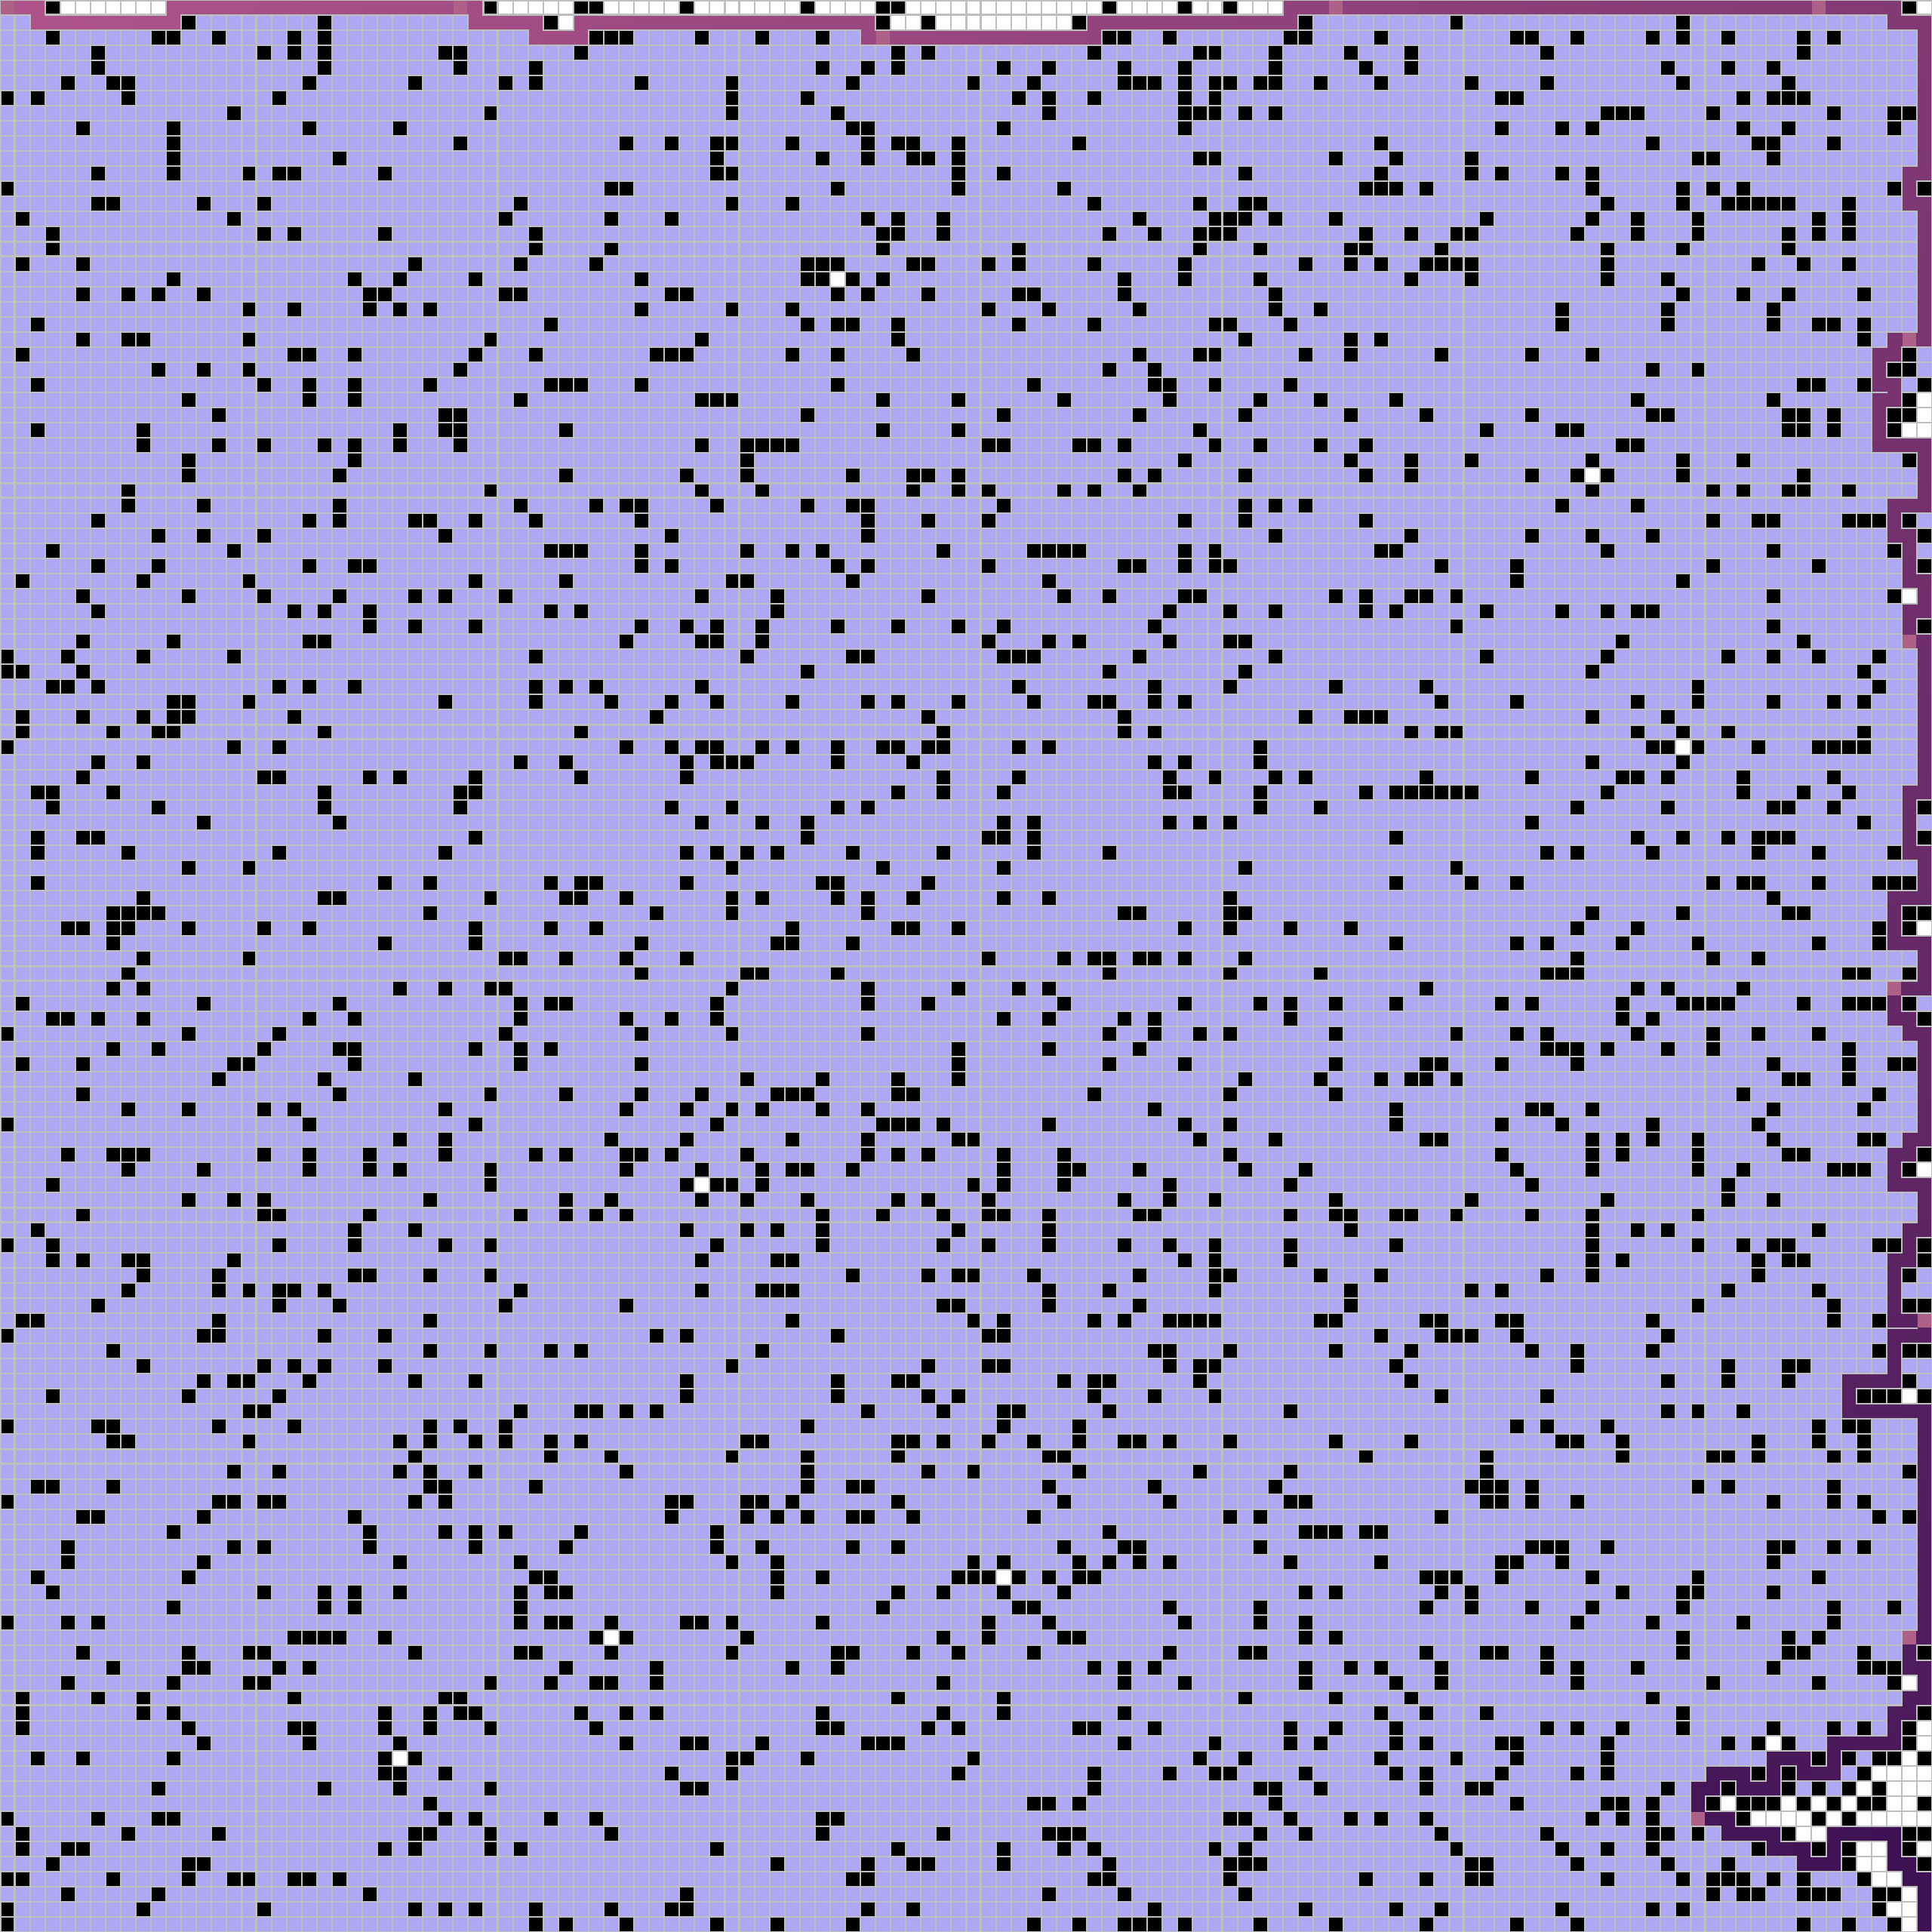
\includegraphics[width=\textwidth]{../pics/df/10032_2.png}
					\caption{\label{fig:df1}A maze that is hard for BFS in terms of space complexity, whose maximum fringe size is 10032. }
					
					\minipage{0.49\textwidth}
					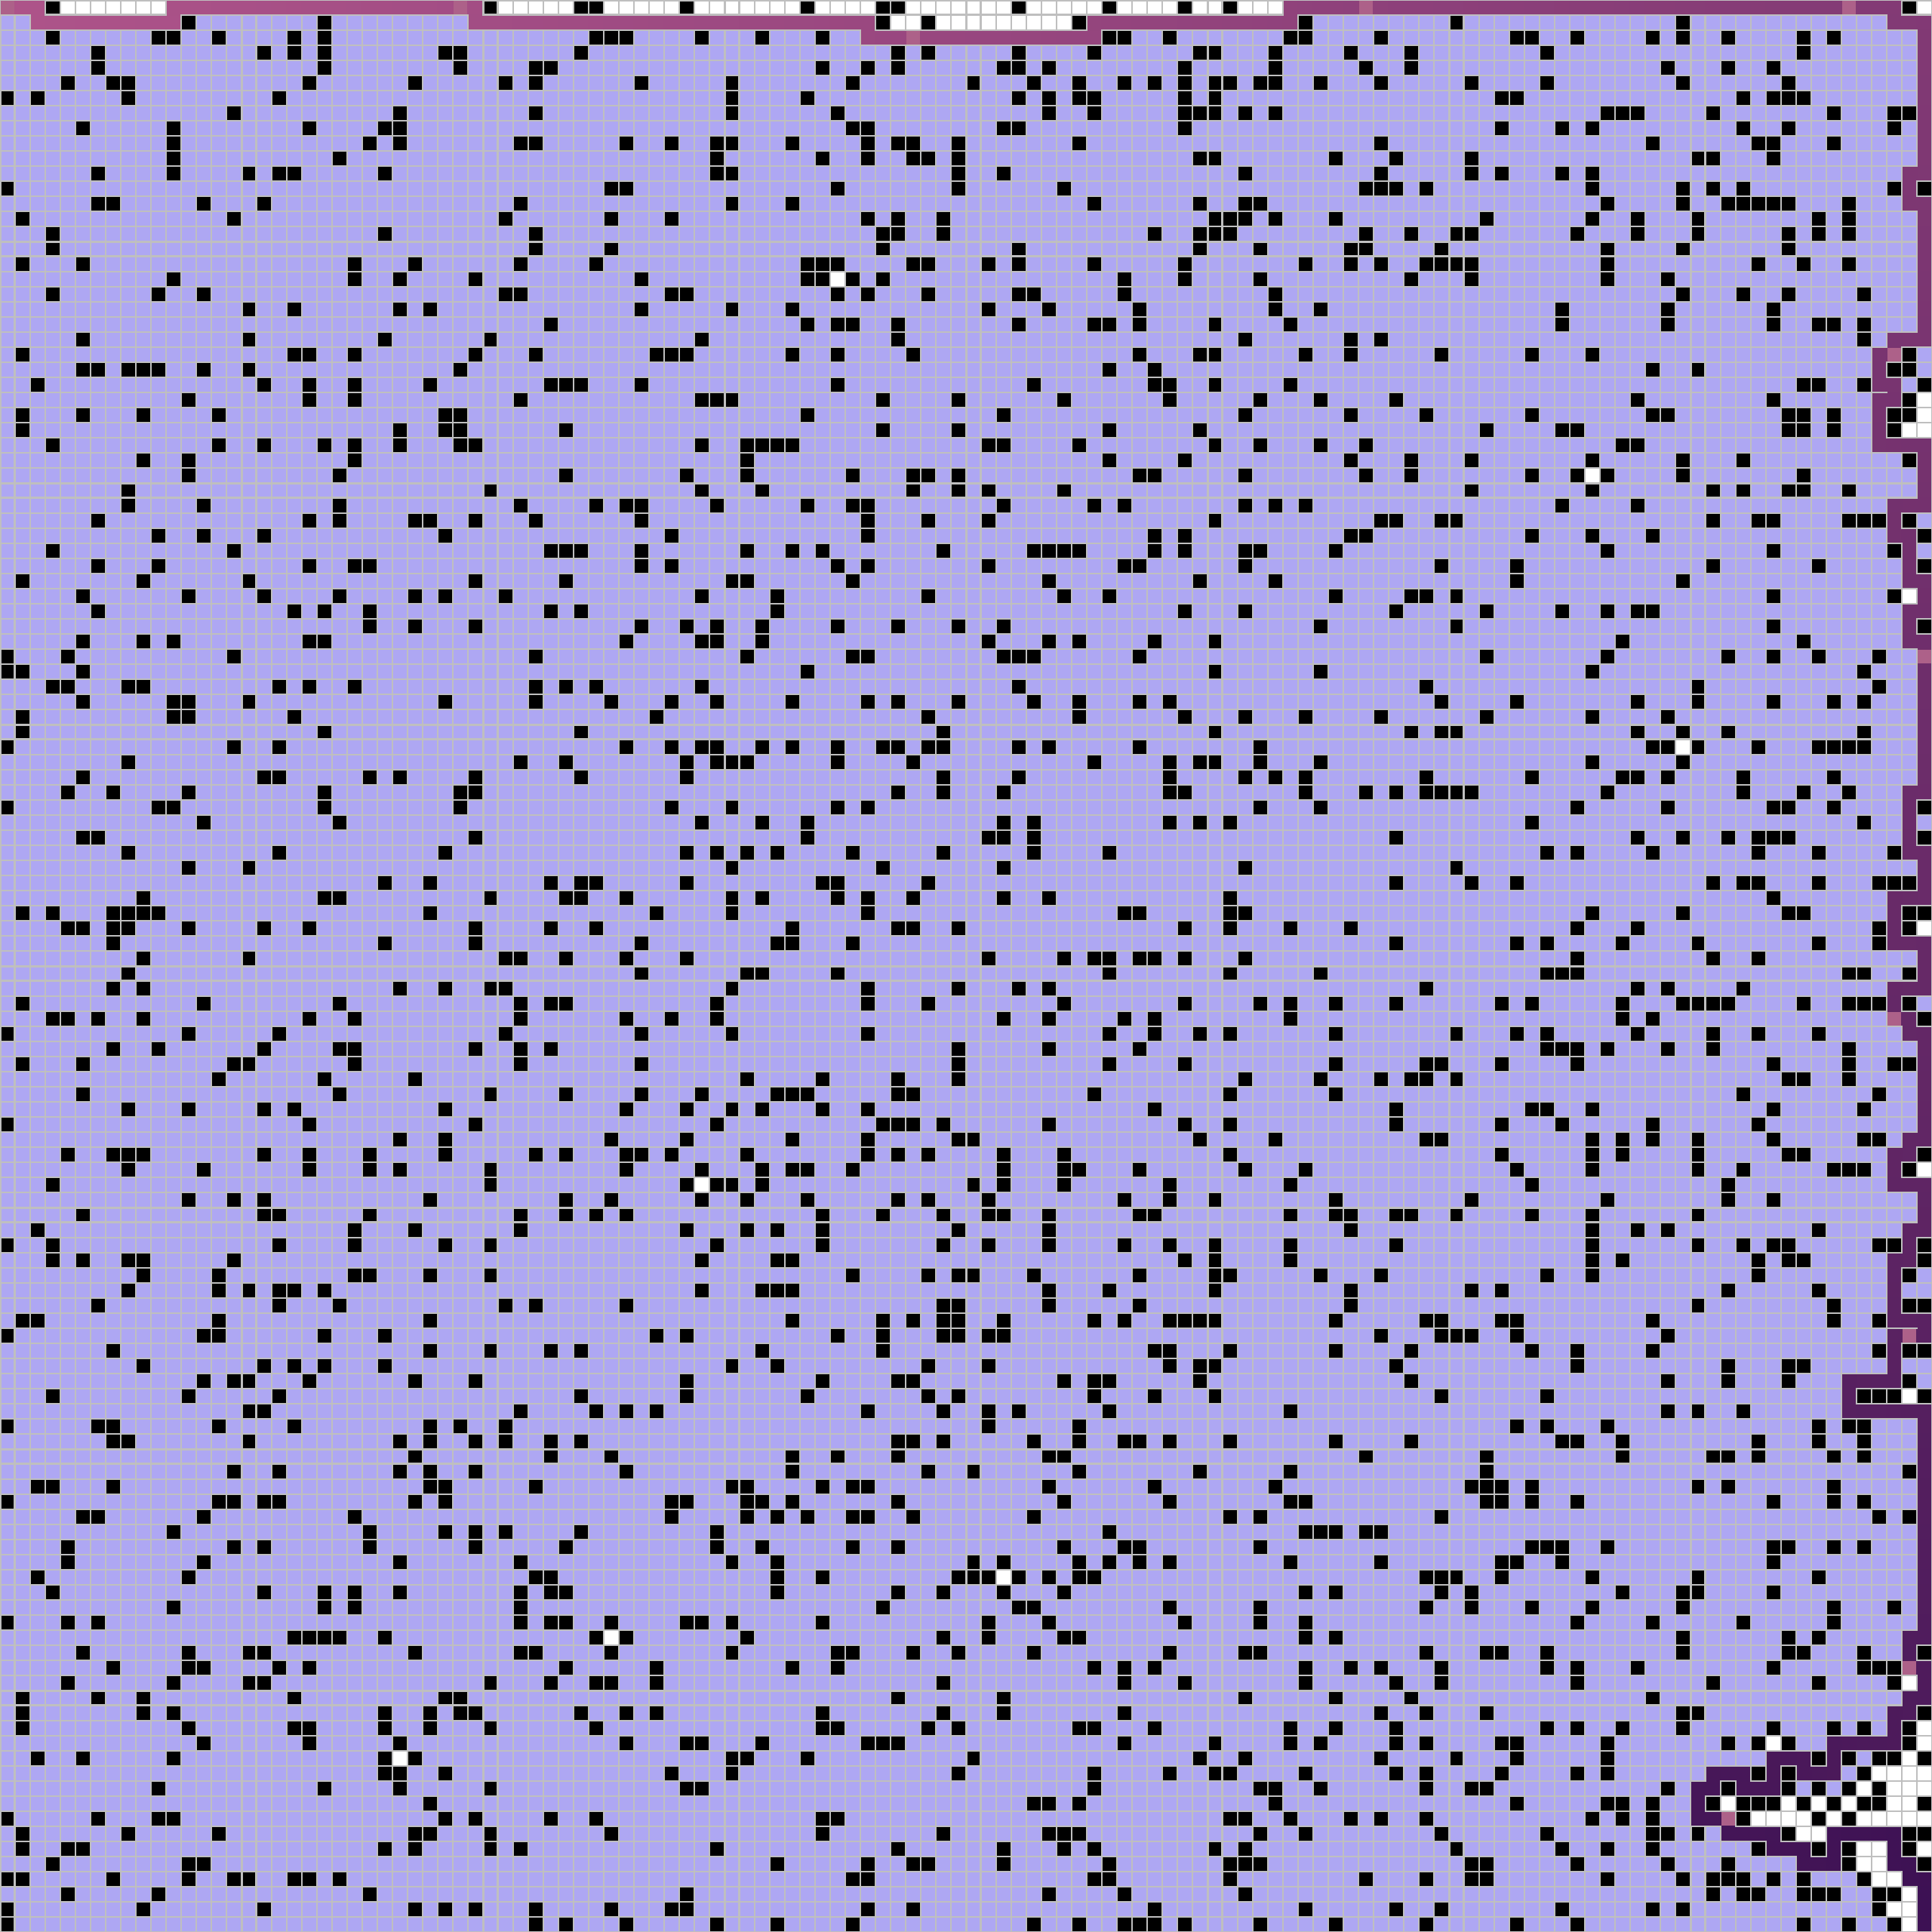
\includegraphics[width=\textwidth]{../pics/df/10032.png}
					\caption{\label{fig:df2}A maze that is hard for BFS in terms of space complexity, whose maximum fringe size is 10032. }
					\endminipage\hfill
					\minipage{0.49\textwidth}
					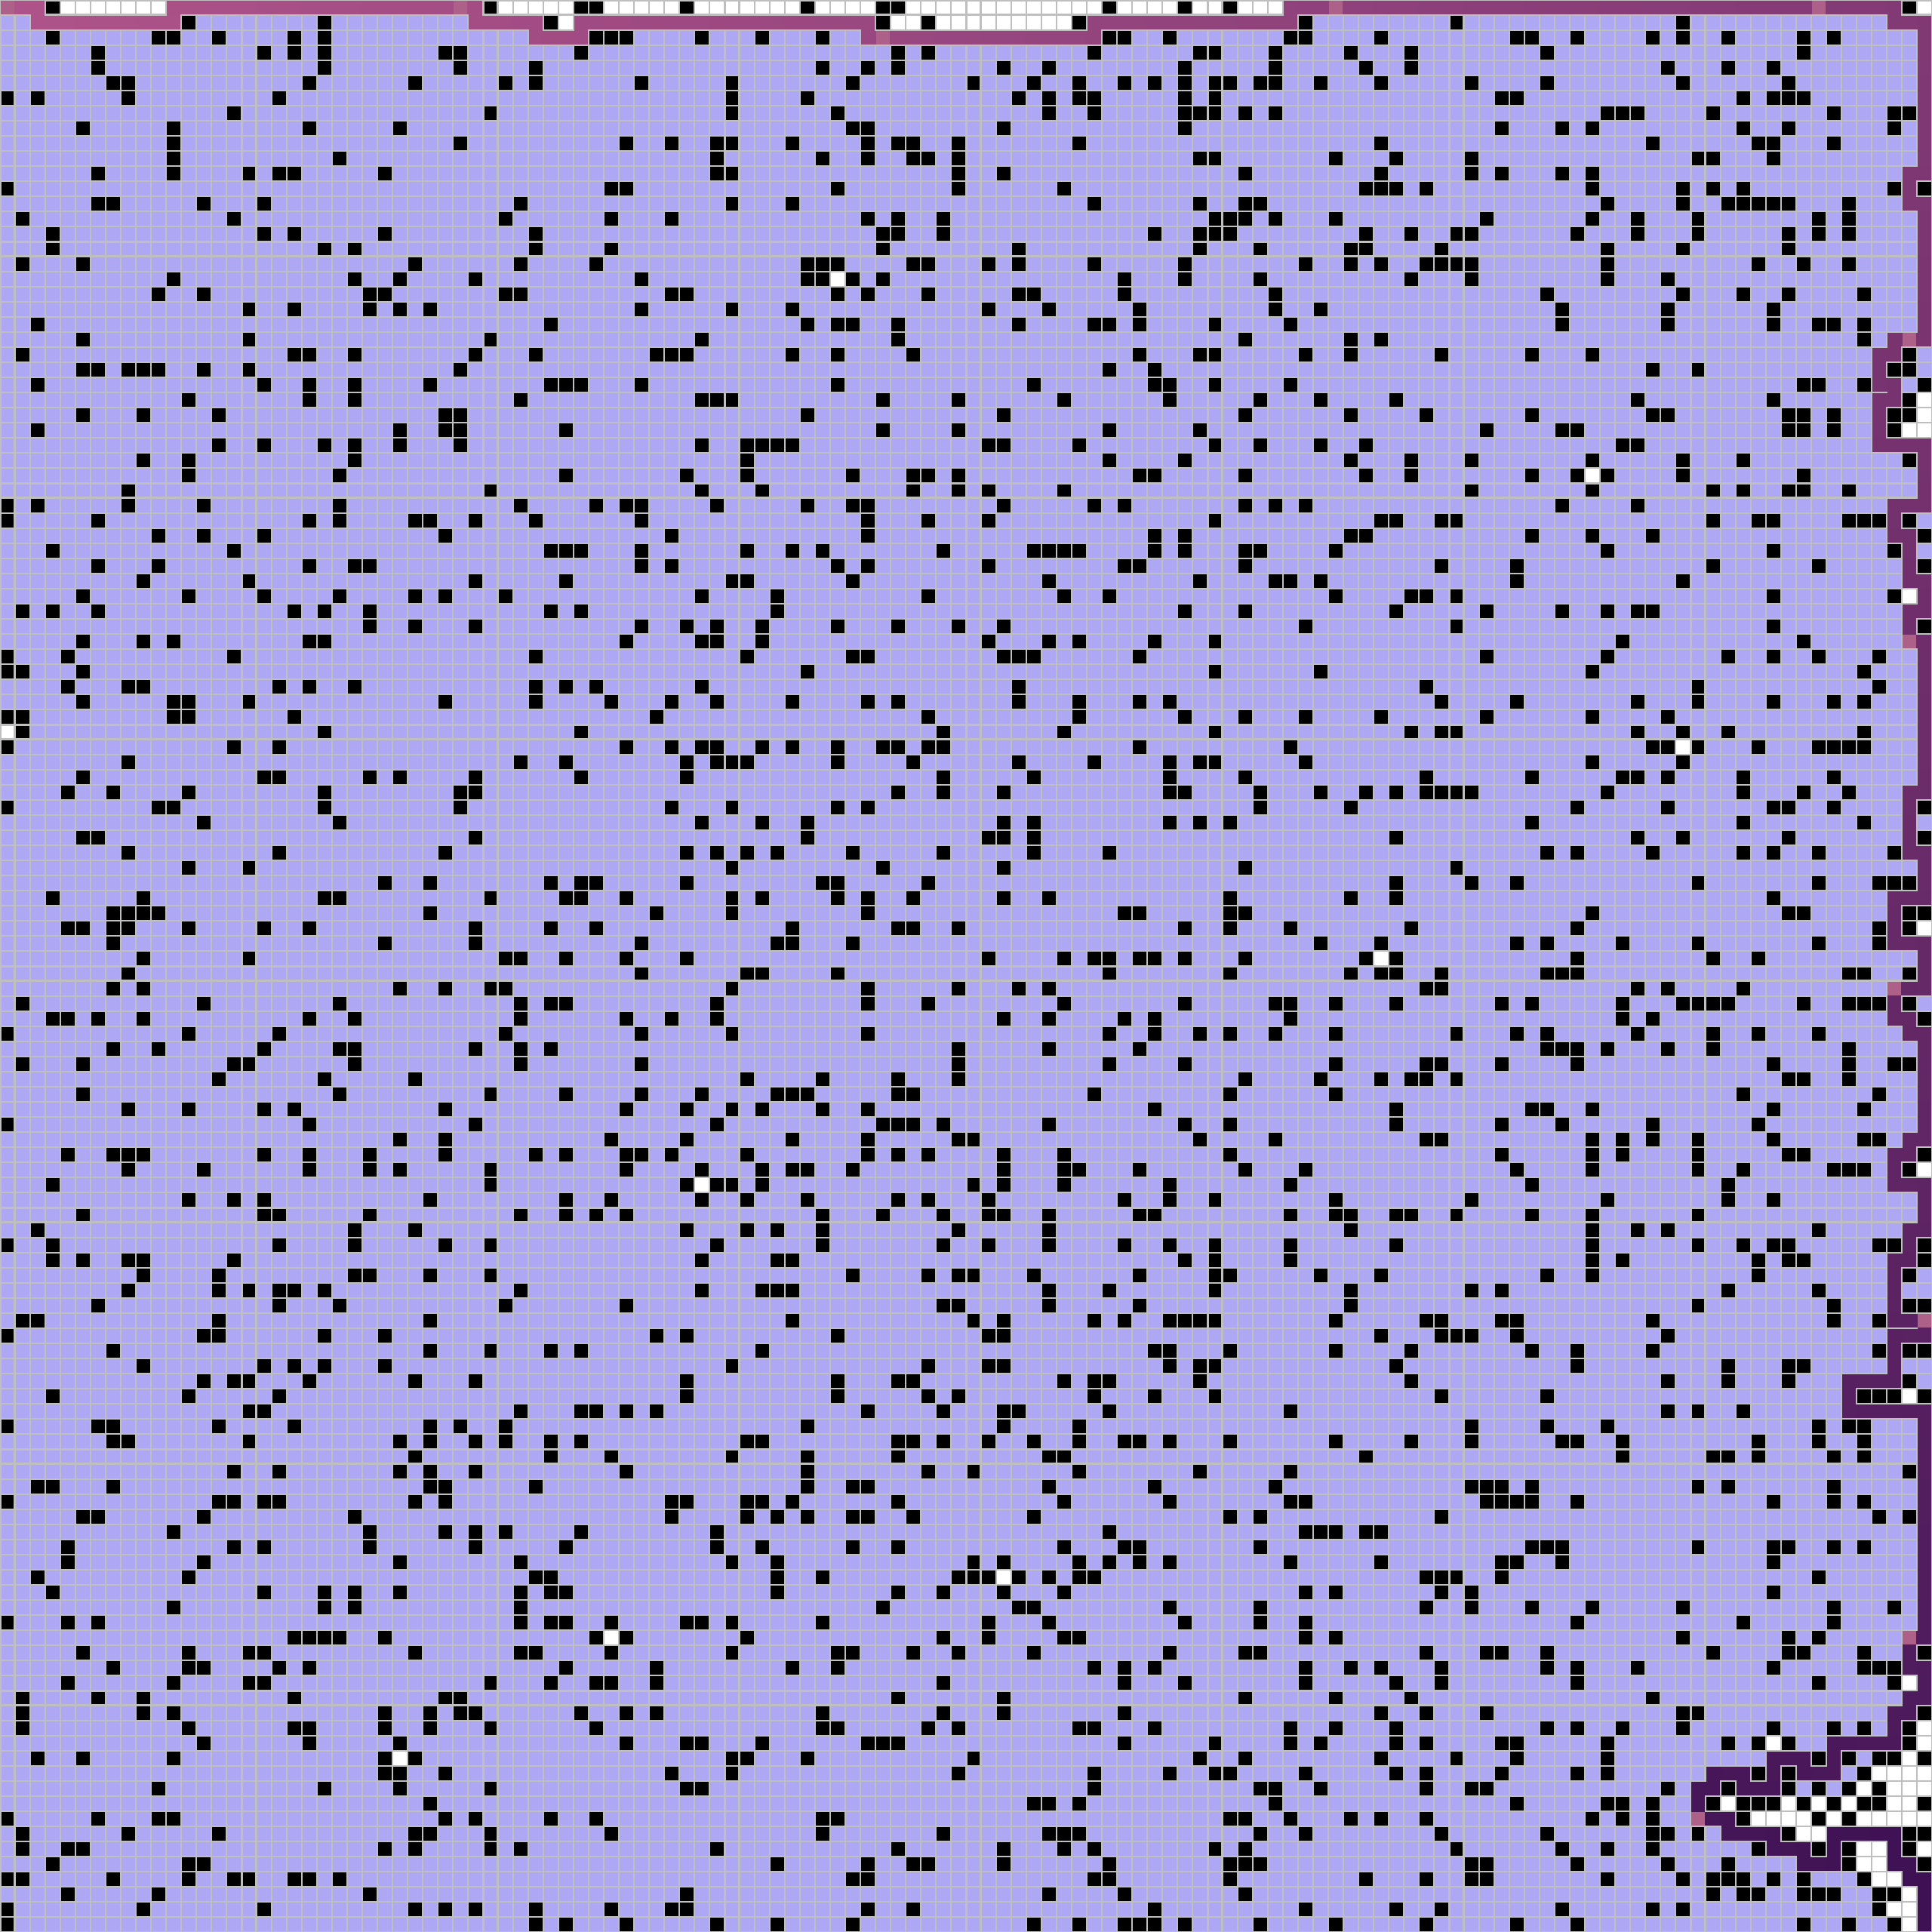
\includegraphics[width=\textwidth]{../pics/df/10031.png}
					\caption{\label{fig:df3} A maze that is hard for BFS in terms of space complexity, whose maximum fringe size is 10031. }
					\endminipage
					\endminipage 
				\end{figure}
				
				\textbf{Patterns or trends:} 
				\begin{itemize}
					\item {The same pattern as Question 10.b.ii, but there should be a clear path along the first row and upper half of the last column.}
				\end{itemize}
				
				\textbf{Reasons:} 
				\begin{itemize}
					\item {The time complexity of DFS related to the maximum depth it has searched.}
					\item {Hence, a "door sill" pattern can force DFS to search lower left part rather than immediately reach the Goal, which increased the maximum depth of DFS.}
					\item {A larger lower left part increases the depth, so the upper right part should be as small as possible.}
				\end{itemize}
				
				\textbf{"The hardest" maze:} 
				\begin{itemize}
					\item {The same maze as Question 10.b.ii.}
					\item {The maximum fringe size is theoretically $(size-1)^2-WallCost = 16113$, compared with 10032. Noticed distinctFringe actually do not promise all elements in the fringe are distinct because it takes too much time to search in a stack frequently. (Further information is available in description.md)}
					\item {Again, it is really difficult to cancel out those outside walls by random without destroying the pattern. Therefore, it has been a nearly "hardest" maze.}
				\end{itemize}
			\end{enumerate}
			
			\item {$ A^* $ with Manhattan Distance Heuristic} 
			\label{A*M}
			\begin{enumerate}
				\item {Length of solution path returned: See Figure \ref{fig:dp1}, Figure \ref{fig:dp2} and Figure \ref{fig:dp3}.} \\
				\begin{figure}
					\minipage{\textwidth}
					
					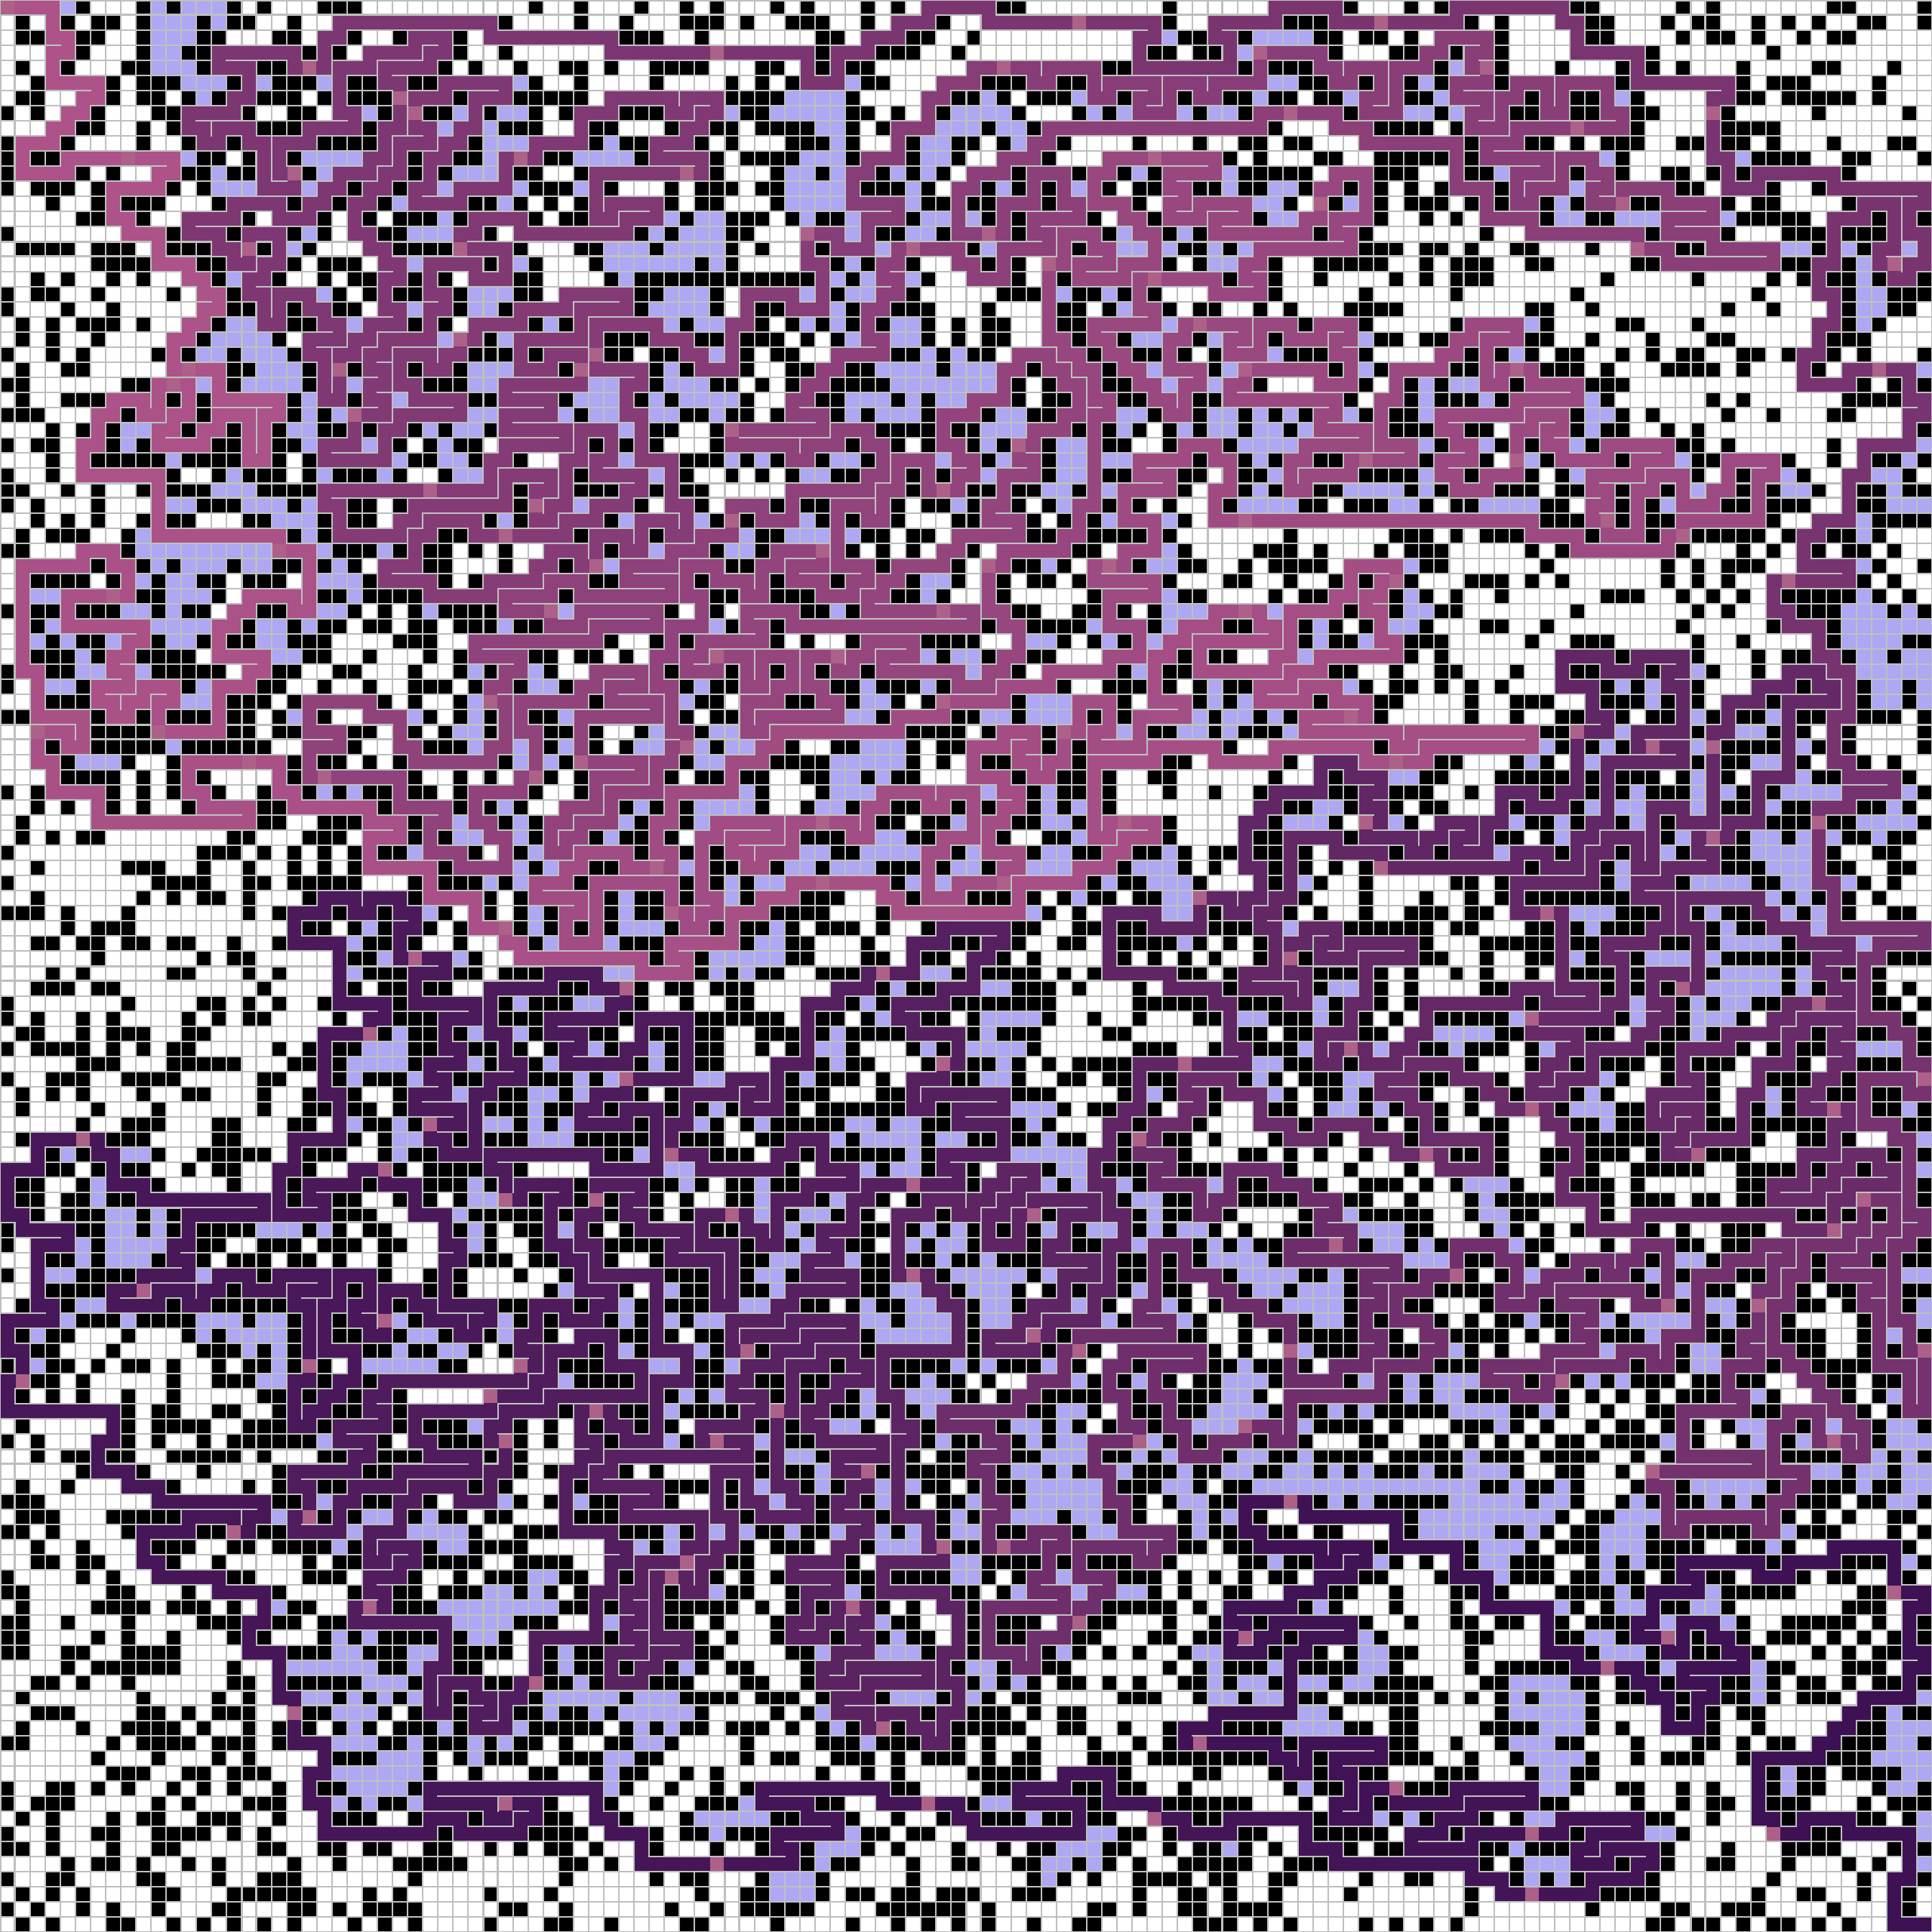
\includegraphics[width=\textwidth]{../pics/dp/5557.png}
					\caption{\label{fig:dp1}maze that is hard for DFS in terms of path length, which is 5557.}
					
					\minipage{0.49\textwidth}
					\includegraphics[width=\textwidth]{../pics/dp/5503.png}
					\caption{\label{fig:dp2}maze that is hard for DFS in terms of path length, which is 5503.}
					\endminipage\hfill
					\minipage{0.49\textwidth}
					\includegraphics[width=\textwidth]{../pics/dp/5495.png}
					\caption{\label{fig:dp3}maze that is hard for DFS in terms of path length, which is 5495.}
					\endminipage
					\endminipage
					
				\end{figure}
				\textbf{Patterns or trends:} 
				\begin{itemize}
					\item {There are 2 classical patterns of walls. (See Figure \ref{fig:dp-pattern}) In one case, walls lead agents to go down some rows, then there usually several nearly "empty"(no walls) rows to move horizontally. But at the end of these rows, diagonal walls lead agents to move up. This case looks like "I" and ">". The other case is "J-shape" walls. }
					\begin{figure}
						\minipage{0.6\textwidth}
						\includegraphics[width=\textwidth]{../pics/dp/pattern.png}
						\caption{\label{fig:dp-pattern}Two classical patterns of walls: "I" and ">" walls and "J-shape" walls.}
						\endminipage\hfill
						\minipage{0.39\textwidth}
						\includegraphics[width=\textwidth]{../pics/dp/hardest.png}
						\caption{\label{fig:dp-hardest}}
						\endminipage
					\end{figure}
					
					\item {"I" and ">" walls and "J-shape" walls appear alternately.}
				\end{itemize}
				
				\textbf{Reasons:} 
				\begin{itemize}
					\item {The key point is when randomWalk == False, the priority of 4 directions is Right > Down > Left > Up.}
					\item {"I" and ">" walls lead agent walk horizontally, and the path it has walked becomes "new wall" because those blocks have been added into the closed set. Now it becomes a "J-shape" walls in the mirror.}
					\item {"J- shape" walls force agents search all blocks inside because agents prefer to go right or left than to move up.}
				\end{itemize}
				
				\textbf{"The hardest" maze:} 
				\begin{itemize}
					\item {The ideal "J-shape" walls can be maze-sized. (See Fig \ref{fig:dp-hardest}) In this case, the path length can be $size \times size - WallCost = 16312$. Notice that if size is an odd number, not all the accessible blocks are in the path. Specifically, only the first 3 blocks in the 2nd row are in the path. }
					\item {Compared with 16312, 5557 is not a big number. However, it is extremely impossible to randomly set all walls in a line.}
					\item {However, compared with less than 1000 block length in a 200 by 200 maze(from Question 5), 5557 in a 128 by 128 maze can be regarded as a "harder" maze, though it is not the "hardest" maze.}
				\end{itemize}
				
				\item {Total number of nodes expanded: See Figure \ref{fig:dp1}, Figure \ref{fig:dp2} and Figure \ref{fig:dp3}.} \\
				\begin{figure}
					\minipage{\textwidth}
					
					\includegraphics[width=\textwidth]{../pics/db/12993.png}
					\caption{\label{fig:db1}A maze that is hard for DFS in terms of time complexity, which has opend 12993 blocks.}
					
					\minipage{0.49\textwidth}
					\includegraphics[width=\textwidth]{../pics/db/12968.png}
					\caption{\label{fig:db2}A maze that is hard for DFS in terms of time complexity, which has opend 12968 blocks.}
					\endminipage\hfill
					\minipage{0.49\textwidth}
					\includegraphics[width=\textwidth]{../pics/db/12967.png}
					\caption{\label{fig:db3} A maze that is hard for DFS in terms of time complexity, which has opend 12967 blocks.}
					\endminipage
					\endminipage 
				\end{figure}
				
				\textbf{Patterns or trends:} 
				\begin{itemize}
					\item {The pathway near the Goal(10 * 10 blocks in the lower right corner) is extremely narrow(only 1 block width), opens to left, and begins with a "door sill" wall that forces the path to move up a block.}
					
					\item {"I" and ">" walls and "J-shape" walls appear alternately.}
				\end{itemize}
				
				\textbf{Reasons:} 
				\begin{itemize}
					\item {Notice that when randomWalk == False, the priority of 4 directions is Right > Down > Left > Up.}
					\item {The pathway opens to left rather than up makes DFS cannot first run right to the last column and then find the pathway. It takes time for DFS to search all upper right part(above the path) and then realize "Oops, there is no way to the goal. I have to backtrack."}
					\item {After DFS reached the "door sill", it prefers to go to any directions but up. Hence, it takes more time for DFS to search all lower left part(below the path) and then realize "Alright, I will go up to see if there is a path."}
					\item {Therefore, DFS nearly searched all the blocks to reach the Goal.}
					\item {Notice that if randomWalk == True, this pattern will not always work because DFS may go down first rather than right.}
				\end{itemize}
				
				\textbf{"The hardest" maze:} 
				\begin{itemize}
					\item {A maze is "empty"(no walls) except the lower right corner. The lower right corner should be a pathway like this pattern. The smallest pattern can be done in 4 * 4.(See Fig \ref{fig:db-hardest}). Notice there must be at least 2 block height "door sill" for DFS to turn back to search lower left part. }
					\begin{figure}
						\centering
						\includegraphics[width=0.3\textwidth]{../pics/db/hardest.png}
						\caption{\label{fig:db-hardest} The smallest pathway pattern.}
					\end{figure}
					\item {Compare to $size \times size - WallCost =16377$, 12993 can still be improved. However, it is really difficult to cancel out those outside walls by random without destroying the pattern. Therefore, it has been a nearly "hardest" maze.}
				\end{itemize}
				
				
				\item {Maximum size of fringe during runtime: See Figure \ref{fig:df1}, Figure \ref{fig:df2} and Figure \ref{fig:df3}.} \\
				\begin{figure}
					\minipage{\textwidth}
					
					\includegraphics[width=\textwidth]{../pics/df/10032_2.png}
					\caption{\label{fig:df1}A maze that is hard for BFS in terms of space complexity, whose maximum fringe size is 10032. }
					
					\minipage{0.49\textwidth}
					\includegraphics[width=\textwidth]{../pics/df/10032.png}
					\caption{\label{fig:df2}A maze that is hard for BFS in terms of space complexity, whose maximum fringe size is 10032. }
					\endminipage\hfill
					\minipage{0.49\textwidth}
					\includegraphics[width=\textwidth]{../pics/df/10031.png}
					\caption{\label{fig:df3} A maze that is hard for BFS in terms of space complexity, whose maximum fringe size is 10031. }
					\endminipage
					\endminipage 
				\end{figure}
				
				\textbf{Patterns or trends:} 
				\begin{itemize}
					\item {The same pattern as Question 10.b.ii, but there should be a clear path along the first row and upper half of the last column.}
				\end{itemize}
				
				\textbf{Reasons:} 
				\begin{itemize}
					\item {The time complexity of DFS related to the maximum depth it has searched.}
					\item {Hence, a "door sill" pattern can force DFS to search lower left part rather than immediately reach the Goal, which increased the maximum depth of DFS.}
					\item {A larger lower left part increases the depth, so the upper right part should be as small as possible.}
				\end{itemize}
				
				\textbf{"The hardest" maze:} 
				\begin{itemize}
					\item {The same maze as Question 10.b.ii.}
					\item {The maximum fringe size is theoretically $(size-1)^2-WallCost = 16113$, compared with 10032. Noticed distinctFringe actually do not promise all elements in the fringe are distinct because it takes too much time to search in a stack frequently. (Further information is available in description.md)}
					\item {Again, it is really difficult to cancel out those outside walls by random without destroying the pattern. Therefore, it has been a nearly "hardest" maze.}
				\end{itemize}
			\end{enumerate}
		\end{enumerate}
	\end{enumerate}
\end{document}